%!TEX root = ../thesis.tex

\chapter{闪电氮氧化物的产率估算} \label{chapter:PE}

由于地表人为排放的NO$_x$需经过传输过程才能抵达自由对流层,进而影响该层的O$_3$浓度,
而闪电直接在对流层中上层产生NO$_x$,该层的低温导致LNO$_x$寿命更长,
所以LNO$_x$可对该层的O$_3$浓度产生更大的影响。
然而,尽管前人针对LNO$_x$开展了一系列研究(见\ref{sec:intro_lnox}节),
由于难以原位观测或实验室重现,所以LNO$_x$的产率仍有很高的不确定性。
本章旨在通过使用卫星观测和云分辨化学模式来改进对LNO$_x$的估算。

本章余下部分按照以下方式组织:
\ref{sec:arctic}节将TROPOMI的NO$_2$观测和GLD360闪电探测数据相结合,
利用TROPOMI在北极地区的相邻过境数据,计算旺盛对流的LNO$_x$产率和产量,并与其他NO$_x$排放源进行对比;
\ref{sec:us}节利用WRF-Chem的高分辨率模拟结果,定义筛选条件和新的AMF,
用于计算美国大陆旺盛对流的LNO$_x$柱浓度和产率;
\ref{sec:china}节在\ref{sec:us}节的基础上计算中国东南部消散对流的LNO$_x$柱浓度和产率,
最后是本章小结。


\section{清洁地区(北极)} \label{sec:arctic}

\subsection{闪电的分布} \label{subsect:lightning_distribution}

全球气候变暖正在引起闪电分布的变化\citep{Reeve.1999,Williams.2005a,Price.2009a}。
在过去的 30 年中,研究学者针对闪电预测提出了多种模拟方案\citep{Price.1992,Price.1997b,Allen.2002,Futyan.2007,Finney.2014,Romps.2014}。
气候模式模拟结果显示,中纬度地区的闪电将有所增加\citep{Michalon.1999,Romps.2014,Luhar.2021},
而在热带地区不同方案的预测结果目前仍存在分歧\citep{Finney.2018,Romps.2019}。
此外,虽然北极地区变暖速度是全球平均水平的4倍\citep{Rantanen.2022},但针对北极闪电的研究还很少。
最近,\citet{Chen.2021a}针对北极地区开发了闪电参数化方案,
结果表明,若本世纪末全球平均气温上升3.7 $^{\circ}$C,永冻区的闪电频率将增加74--150\%。
地基闪电观测结果显示,北极闪电相对于全球闪电的比例在2010至2020年期间增加了两倍\citep{Holzworth.2021}。
此外,北极地区在夏季将有更多的水汽辐合来加强对流系统,从而导致更多的闪电\citep{Bintanja.2020}。

为了研究北极地区的闪电变化,我们将光学瞬态探测器(OTD,1996--1999)的卫星闪电数据
与维萨拉全球地基雷电数据集(GLD360,2019--2021)进行比较。
其中OTD的数据产品为闪电次数,一次闪电可包含一个或多个闪击。
虽然GLD360官方产品只包含闪击,但是我们的目的是研究闪电分布的变化,故未将闪击聚类成闪电。
GLD360数据覆盖了整个高纬度地区($>$60$^{\circ}$ N),而OTD仪器只观测75$^{\circ}$ N以南的闪电。
在2019--2021年夏季(6月至8月)GLD360探测到75$^{\circ}$ N 以北发生的闪击所占比例为3\%(图\ref{fig:gld360_tseries})。

\begin{figure}[H]
\centering
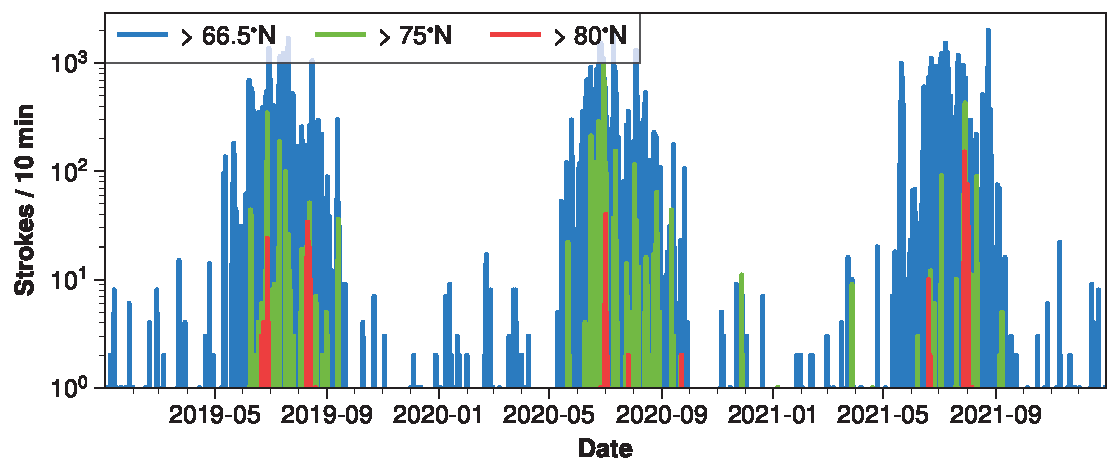
\includegraphics[width=0.75\textwidth]{./figures/arctic_gld360_tseries.png}
\caption{
GLD360探测的每10分钟闪击时间序列。\\
Figure \ref{fig:gld360_tseries}. Time series of GLD360 lightning strokes per 10 minutes.
}
\label{fig:gld360_tseries}
\end{figure}


如图\ref{fig:arctic_lightning_distribution}所示,我们比较了卫星和地基闪电网在高纬度地区观测到的夏季闪电空间分布。
两个数据集均显示北极野火的主要发生地[西伯利亚和阿拉斯加永冻区,
\citep{McCarty.2021}]具有较高的闪电频率(图\ref{fig:arctic_lightning_distribution}a,b)。
OTD测得的平均闪电频率和GLD360测得的平均闪击频率分别为0.22 km$^{-2}$每月和0.61 km$^{-2}$每月。
然而,OTD 在楚科奇海(Chukchi Sea)附近记录的闪电较少,但在伊明格海(Irminger Sea)上空较多。
该现象与北极降水的年际变化和向极地输送的水汽有关\citep{Bintanja.2020}。

为了判断 TROPOMI 是否可以探测到 LNO$_2$,我们首先计算了每次TROPOMI过境前3 h内条带内发生的GLD360闪击数。
由于TROPOMI在北极地区每天有14条重叠条带,条带内的闪击数约占总数的 9\%(图\ref{fig:arctic_lightning_distribution}c),并且具有相同的地理分布(图\ref{fig:arctic_lightning_distribution}b)。
纬度越高,条带内闪击的占比越大(图\ref{fig:arctic_lightning_distribution}d),
从$<$ 10\%(60--70$^{\circ}$ N)增加到 10--25\%(70--80$^{\circ}$ N)和40--100\%(80--90$^{\circ}$ N)。
由于地基观测\citep{Schmale.2018} 和飞机观测\citep{Jacob.2010}的NO$_2$数据有限,
因此TROPOMI的观测数据在分析北极地区的 LNO$_2$ 方面十分有利。
鉴于 70$^{\circ}$ N 以北具有更高的 TROPOMI 覆盖率和更少的其他NO$_2$排放源(例如野火或天然气),我们选择该区域来计算LNO$_2$ 产率。
如表\ref{table:arctic_emission}所示,GLD360在70$^{\circ}$ N 以北探测到的夏季闪击数分别为 1.2$\times$10$^6$ (2019)、1.6$\times$10$^6$ (2020) 和 9.8$\times$10$^5$ ( 2021)。
其中在TROPOMI 覆盖率最高的地区(80--90$^{\circ}$ N),2021 年的闪击数约为 2.9$\times$10$^4$,是前九年总数的近两倍\citep{networktotal.2021}。
GLD360测得的闪击最北可达89.5$^{\circ}$ N,WWLLN也探测到了该次闪击[89.6 $^{\circ}$ N,\citet{Holzworth.2021}]。


\begin{figure}[H]
\centering
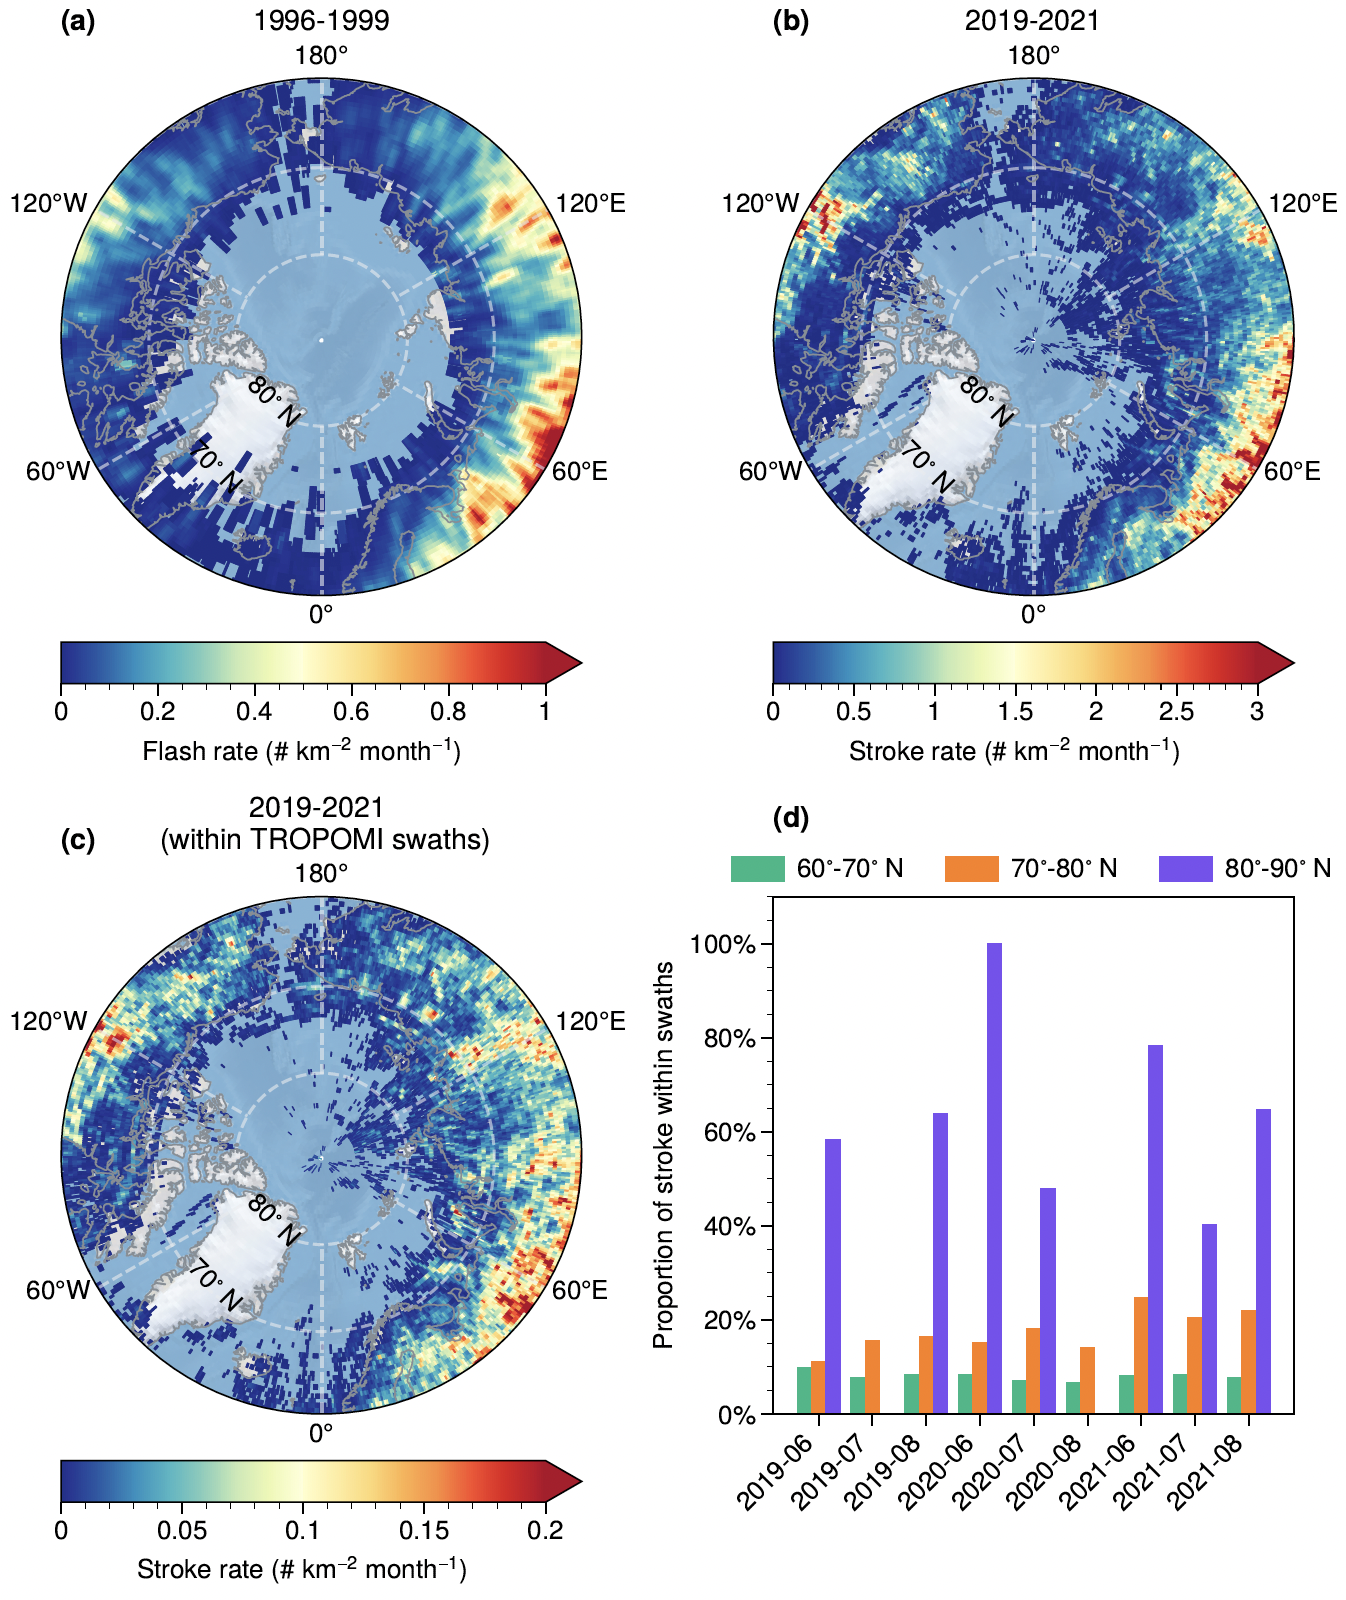
\includegraphics[width=0.8\textwidth]{./figures/arctic_lightning_distribution.png}
\caption{
(a)1996至1999年6-8月OTD观测的平均闪电频率;
(b)2019至2021年6-8月GLD360观测的平均闪击频率;
(c)与(b)相同,但只计算TROPOMI过境前3 h内TROPOMI条带内的闪电;
(d)为(c)与(b)的月比例。\\
Figure \ref{fig:arctic_lightning_distribution}.
(a) Mean OTD lightning flash rate of June--August 1996--1999;
(b) Mean GLD360 lightning stroke rate of June--August 2019--2021;
(c) Same as panel b but only counting the lightning inside the TROPOMI swaths during the 3 h period before the TROPOMI overpass time.
Grids with no lightning appear as the light-blue backgrounds in panels a--c.
(d) Monthly ratio of panel c to panel b.
}
\label{fig:arctic_lightning_distribution}
\end{figure}

\subsection{闪电氮氧化物的计算} \label{sec:arctic_lnox_calc}

LNO$_2$的估算包括以下三个主要步骤:

(1) 使用风场数据将NO$_2$柱浓度高值区与闪电数据匹配。

(2) 基于新算法来计算LNO$_2$柱浓度。

(3) 使用连续的TROPOMI观测数据来计算LNO$_2$的产率。

\begin{table}[H]
\centering
\caption{2019至2021年6--8月北极地区GLD360探测到的闪击数、闪电NO$_2$排放(吨氮)和平均对流有效位能(CAPE,J kg$^{-1}$)\\
Table \ref{table:arctic_emission}. GLD360 stroke counts, lightning NO$_2$ (LNO$_2$) emissions (Mg of N), and mean
convective available potential energy (CAPE, J kg$^{-1}$) in the Arctic region during June--August 2019--2021.
}
\label{table:arctic_emission}
\footnotesize
% \renewcommand{\arraystretch}{0.6}
\begin{tabular}{llllll}
\hline
{} & 70--75$^{\circ}$ N & 75--80$^{\circ}$ N &
80--85$^{\circ}$ N &  85--90$^{\circ}$ N &  \\
\hline
闪击 & & & & & 总数 \\
\hline
2019 &   1,142,292 &     40,660 &      5,756 &       636  & 1,189,344 \\
2020 &   1,402,304 &    233,780 &      4,784 &       768  &  1,641,636 \\
2021 &     889,248 &     62,296 &     26,576 &      2,536  &  980,656 \\
\hline
闪电NO$_2$排放 & & & & & 总数 \\
\hline
2019 &      87.3 &       5.6 &       0.9 &       0.1 &   93.9 \\
2020 &      85.5 &      22.1 &       0.8 &       0.1 &  108.5 \\
2021 &      58.6 &       8.6 &       3.9 &       0.4 &   71.5 \\
\hline
对流有效位能 & & & & & 平均值 \\
\hline
2019 & 5.5  & 4.0  & 5.0  & 6.5 & 5.3 \\
2020 & 9.2  & 5.1  & 5.0  & 5.2 & 6.1 \\
2021 & 7.3  & 4.8  & 5.5  & 7.2 & 6.2 \\
\hline
\end{tabular}
\end{table}

\subsection*{闪电的聚类}

我们使用密度聚类算法(DBSCAN)将TROPOMI过境前12 h内\citep{Allen.2021a}的闪击以40 km进行聚类\citep{backlund2011density,Schubert.2017}。
由于野火也会产生 NO$_2$,因此使用可见光/红外成像仪/辐射计套件(VIIRS)375 m 主动火点产品,
来识别和过滤受野火排放影响的闪电聚类。
VIIRS 搭载在 Suomi 国家极地轨道合作伙伴 (Suomi-NPP)上,
它与搭载TROPOMI的S5P位于同一轨道,但比 S5P 提前3.5分钟。
我们将内部没有火点的闪电集群视为一个清洁的聚类。

对于每个清洁的闪电聚类,我们根据观测到的闪击所处位置及发生时间,
在三个气压层(300、500和700 hPa)上定义受 LNO$_2$ 影响的空气块(图 \ref{fig:workflow}a)。
如图 \ref{fig:workflow}b 所示,我们使用 ECMWF 小时大气再分析资料(ERA5) 的风场数据\citep{Hersbach.2020},
对含LNO$_2$ 的空气块进行水平平流输送,并得到TROPOMI 过境时空气块的位置。
最终的空气块组成一个闪电掩膜(图 \ref{fig:workflow}c中的橙色圆圈),即三个等压面的前向轨迹构成了一个近似的 LNO$_2$ 区域。

我们首先使用分水岭方法得到对流层NO$_2$垂直柱浓度($V_{\ch{NO2}}$)的高值区(图 \ref{fig:workflow}c中的像素)。
具体而言,分水岭方法将输入数据视为地形表面,并将它们分成单独的区域,称为集水盆地\citep{Soille.1990,Heikenfeld.2019a}。
在本研究中,我们应用从 4$\times$10$^{14}$ 到 1$\times$10$^{15}$ molec. cm$^{-2}$ 的阈值,步长为 2$\times$10$^{14}$ molec. cm$^{-2}$来检测多个局部NO$_2$高值特征。
这些特征用于识别具有高 $V_{\ch{NO2}}$ 的附近区域(图 \ref{fig:workflow}c 中不同颜色的像素)。
接着我们选择包含一个或多个高 $V_{\ch{NO2}}$ 区域的掩膜用于 LNO$_2$ 的进一步分析,
最终对闪电掩膜内的数据用分水岭方法进行重新识别,得到具有高 $V_{\ch{NO2}}$ 的LNO$_2$ 区域(图 \ref{fig:workflow}d 中的亮色像素)。


\begin{figure}[H]
\centering
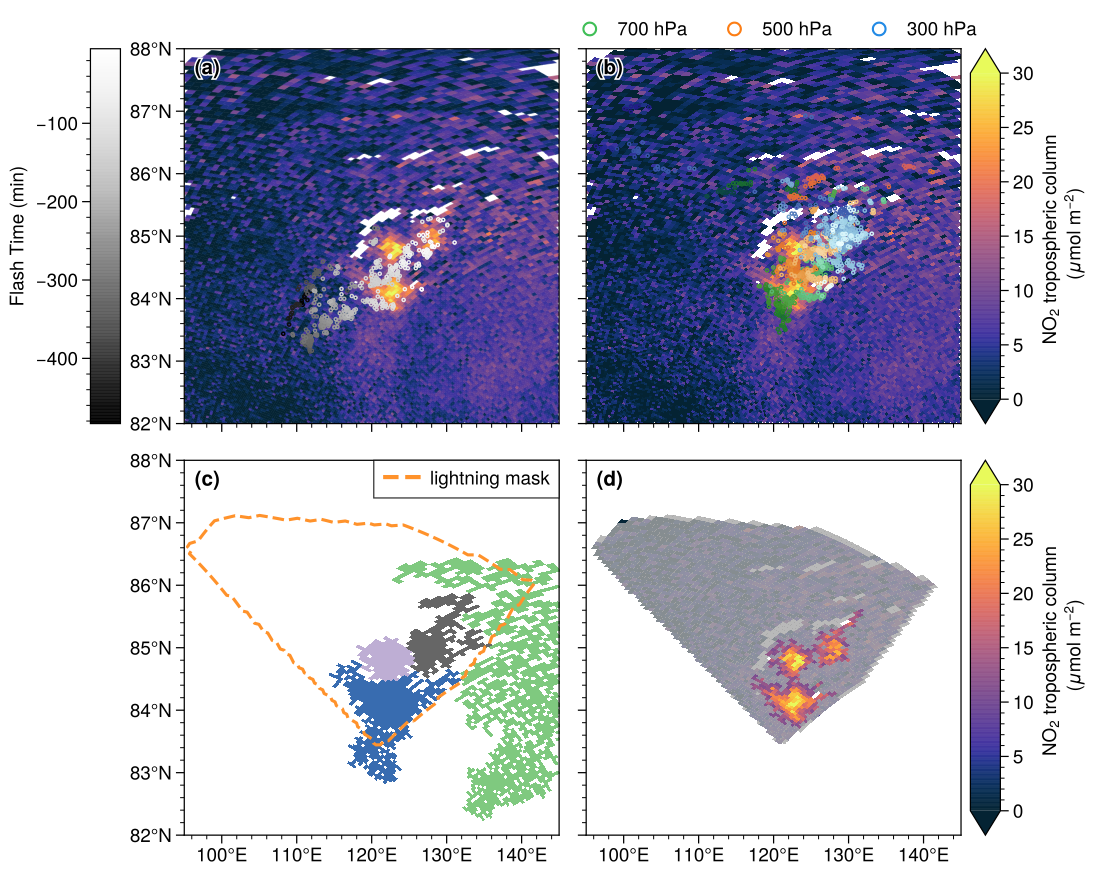
\includegraphics[width=0.85\textwidth]{./figures/arctic_workflow.png}
\caption{
从 TROPOMI 轨道 09458(2019 年 8 月 1 日)数据筛选闪电 NO$_2$ 像素的示意图。
背景填色为TROPOMI 检测到的 NO$_2$ 对流层柱浓度,
(a)观测到的闪击;
(b)在三个气压层(300 hPa、500 hPa 和 700 hPa)上水平传输的闪电 NO$_2$ 空气块;
(c)将空气块组合成一个闪电掩膜(橙色框),与高 NO$_2$高值区(填充像素)重叠。
不同的像素颜色代表基于多个 NO$_2$ 阈值的不同 NO$_2$ 选区;
(d)掩膜内受闪电 NO$_2$ 影响的 NO$_2$ 对流层柱浓度最终选区(亮色像素)。\\
Figure \ref{fig:workflow}. Overview of the process for identifying lightning NO$_2$ pixels from TROPOMI orbit 09458 on August 1, 2019.
The TROPOMI-detected NO$_2$ tropospheric columns are overlaid with (a) observed lightning strokes and
(b) transported air parcels of lightning NO$_2$ at three pressure levels [300 hPa (blue), 500 hPa (orange), and 700 hPa (green)].
(c) Parcels are combined into one lightning mask (orange circle), which overlaps with high NO$_2$ selections (filled pixels). The different pixel colors represent different NO$_2$ selections based on multiple NO$_2$ thresholds.
(d) Final selection (bright colored pixels) of NO$_2$ tropospheric columns affected by lightning NO$_2$ within the mask.
}
\label{fig:workflow}
\end{figure}

在重新使用分水岭方法之前,我们使用最小--最大归一化将掩膜内的 $V_{\ch{NO2}}$ 值归一化为 0--1 的范围,即从每个数据中减去最小值并除以最大值和最小值之间的差值。
我们将对数正态分布模型拟合到置信度为 80\% 的归一化值,并将结果用作分水岭过程的最小阈值。
由于 LNO$_2$ 区域通常小于闪电掩模(图 \ref{fig:workflow}d),
80\% 的置信水平应足以识别 LNO$_2$ 像素。
与置信度相关的不确定性见表 \ref{table:arctic_uncertainty}。
最后,我们将分水岭算法应用于标准化的 $V_{\ch{NO2}}$ 值,使用的阈值范围从最小值到 1,步长为 10,
这使我们能够识别和分析最终的LNO$_2$数据。


\subsection*{计算闪电氮氧化物柱浓度}

\citet{Zhang.2022a}指出官方 TROPOMI 算法在 NO$_2$反演中不包括 LNO$_2$,
因此我们从官方 $S_{\ch{NO2}}$产品中减去背景 NO$_2$,并将差值通过大气质量因子(AMF)转换为对流层LNO$_2$垂直柱浓度。
该算法具体为下式
\begin{equation} \label{eq:arctic_LNO2}
V_{\ch{LNO_2}} = \frac{S_{\ch{NO_2}} - S_{\ch{BG}}}{AMF_{\ch{LNO_2}}}
\end{equation}
其中 $V_{\ch{LNO2}}$ 是对流层 LNO$_2$ 垂直柱浓度,
$S_{\ch{NO2}}$ 是 TROPOMI 测得的对流层 NO$_2$ 斜柱浓度,
$AMF_{\ch{LNO2Clean}}$ 是闪电大气质量因子。
根据\citet{Allen.2021a}的研究,我们将背景 $S_{\ch{NO2}}$($S_{\ch{BG}}$)定义为对流层 AMF 和在闪电掩膜内NO$_2$低值区的第 30 个百分位数$V_{\ch{NO2}}$的乘积。
NO$_2$低值区(图 \ref{fig:workflow}d中的灰色像素)是由分水岭方法得到的$V_{\ch{NO2}}$高值区之外的所有掩膜像素。
$AMF_{\ch{LNO2Clean}}$ 是“可见”LNO$_2$ 斜柱浓度与对流层 LNO$_2$ 垂直柱浓度之比,即式(\ref{eq:AMF_LNO2clean})。
其中$LNO_2(p)$ 是与气压有关的先验 LNO$_2$高斯分布廓线,
我们将高斯分布的峰值高度设置为闪电掩模中最高的TROPOMI云压,峰值宽度设置为180 hPa。
该峰值宽度是通过高斯分布拟合前人的LNO$_x$廓线得到的,具体如下:
高斯分布由方程 $k*e^\frac{{-{(p - peak\_pressure)}^2}}{2*peak\_width^{2}}$ 给出,
在这个等式中,系数 $k$ 在 AMF 计算中同为分子和分母所以被抵消,$p$ 是TM5-MP的气压层。
利用该公式拟合 \citet{Ott.2010} 的海洋型LNO$_x$廓线和\citet{Luo.2017}的中纬度大陆型LNO$_x$廓线,
得到$peak\_width$ 的平均值为180 hPa(图\ref{fig:arctic_lnox_profile})。
我们没有使用\citet{Ott.2010}中的中纬度大陆 LNO$_x$ 廓线,是由于\citet{Luo.2017}指出该廓线与对流前的廓线相似,而本研究需要对流时的廓线。
与 $peak\_width$ 和云压相关的 LNO$_2$ 生产效率的不确定性见表\ref{table:arctic_uncertainty}。
$AMF_{\ch{LNO2}}$计算中使用的散射权重由五个参数决定:地表气压、太阳天顶角、视角天顶角、相对方位角和反照率。
对于多云部分,查找表中使用的地表气压和反照率采用云压和云反照率。
此外,我们剔除了云层高于对流层顶的个例,因为 NO$_2$ 浓度可能会受到平流层 O$_3$ 的影响\citep{Frey.2015a,Zhang.2022a}。


\begin{figure}[H]
\centering
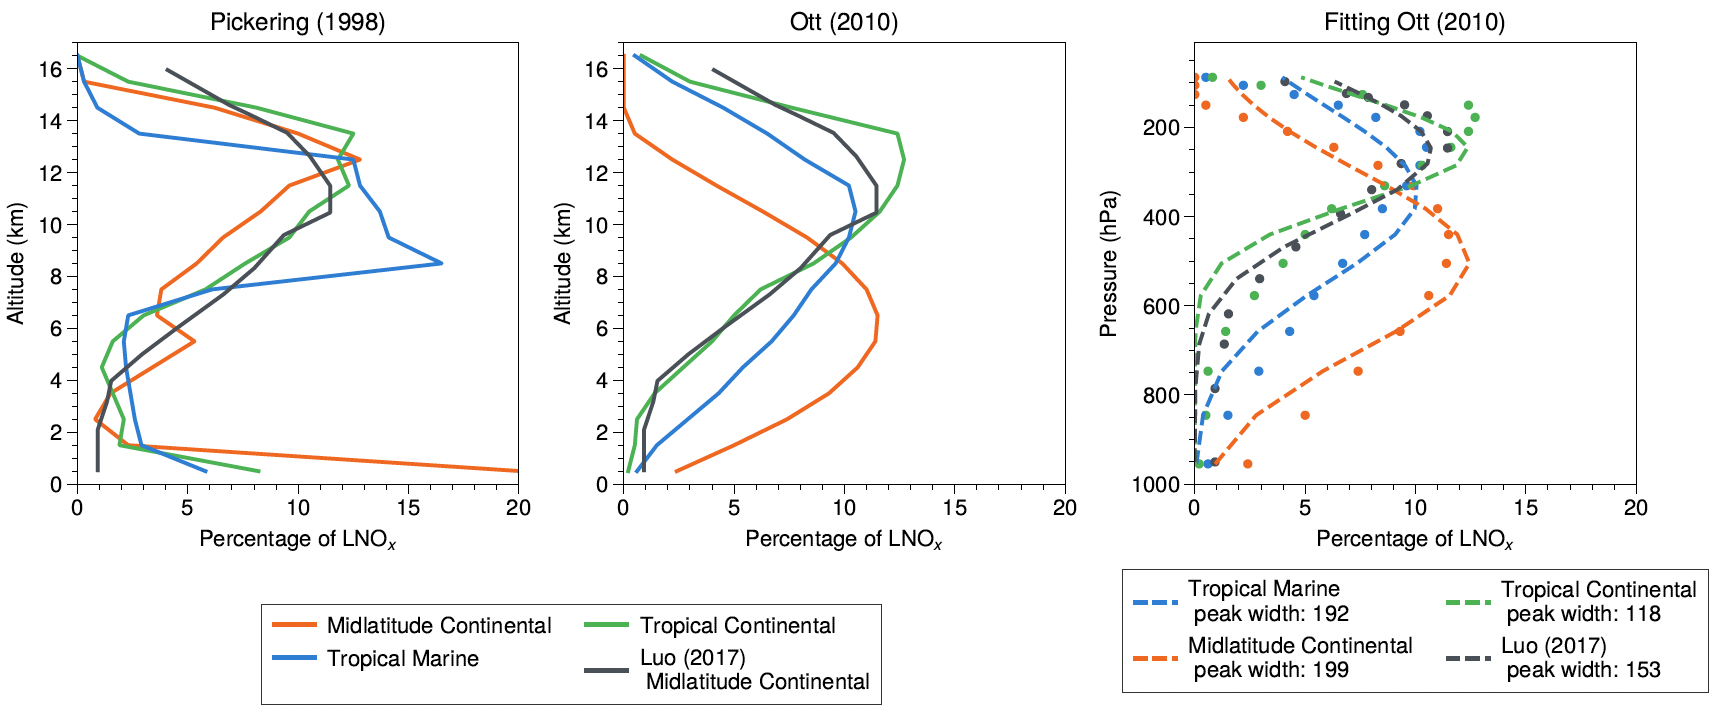
\includegraphics[width=\textwidth]{./figures/arctic_lnox_profile.png}
\caption{
每公里LNO$_x$质量百分比的平均垂直分布。
数据来源:(a)\  \citet{Pickering.1998};(b)\  \citet{Ott.2010},
来自\  \citet{Luo.2017} 的 LNO$_x$ 配置文件以黑色显示;
(c) 高斯拟合曲线(虚线)和原始数据(散点)。\\
Figure \ref{fig:arctic_lnox_profile}.
Average vertical distributions of percentage of typical LNO$_x$ mass per kilometer.
The LNO$_x$ profiles are from (a)\  \citet{Pickering.1998} and (b)\  \citet{Ott.2010}.
The LNO$_x$ profile from\  \citet{Luo.2017} is shown in black.
(c)  The Gaussian fitting profiles (dashed lines) and the original data (scatter points).
}
\label{fig:arctic_lnox_profile}
\end{figure}


\subsection*{计算闪电氮氧化物产率} \label{sec:calc_lnox_pe}

如\ref{subsect:lightning_distribution}节所述,TROPOMI 可多次扫过 70$^{\circ}$ N 以北的同一点,
因此两个连续的轨道可以观测到相同的雷暴系统。
为了更方便地分析北极 LNO$_2$ 案例的模式和变化,我们创建了可视化网站(\url{https://arctic-lightning-no2.streamlit.app/}),
允许用户筛选个例和以交互的方式研究LNO$_2$、云压和闪电之间的关系。
$V_{\ch{LNO2}}$(mol m$^{-2}$)在相邻过境时间之间的关系可以定义为:
\begin{equation} \label{eq:relationship}
\sum_{p_{(T2)}} V_{\ch{LNO_2_i}} A_{i} = e^\frac{{-(T_2-T_1)}}{\tau} \sum_{p_{(T1)}} V_{\ch{LNO_2_j}} A_{j} + PE \sum_{N} e^\frac{{-(T_2-t_k)}}{\tau}
\end{equation}
其中 $p$ 是 LNO$_2$ 区域中的像素数,
$A$ 是每个像素的面积(m$^2$),
$T$ 是 TROPOMI 过境时间,
$t$ 是闪电发生的时间,
$\tau$ 是对流附近 LNO$_2$ 的寿命,
$PE$ 是 LNO$_2$ 的产率(mol NO$_2$ 每闪击),
$N$ 是发生在相邻过境时间内的总闪击数,
而指数成分考虑了 NO$_2$ 的化学损失。
除此之外,$i$ 和 $j$ 是 TROPOMI 的像素索引,
$A_{i}$ 和 $A_{j}$ 是不同的 LNO$_2$ 区域,并考虑了平流的影响(图\ref{fig:consecutive_orbits}),
$T_1$ 和 $T_2$ 代表 TROPOMI 在 LNO$_2$ 区域的两次平均过境时间,
$t_k$ 代表两个轨道之间发生的第 k 次雷击(k 取值范围为 1 到 N)的时间。

如果相邻过境时间内没有闪电发生,式(\ref{eq:relationship})可以简化为:
\begin{equation} \label{eq:LNO2_nolightning}
\sum_{p_{(T2)}} V_{\ch{LNO_2}_i} A_{i} = e^\frac{{-(T_2-T_1)}}{\tau} \sum_{p_{(T1)}} V_{\ch{LNO_2}_j} A_{j}
\end{equation}
我们通过分析具有高 LNO$_2$ 但两次过境时间之间没有闪电的特殊个例,得到 $\tau$ 的值为 3 $\pm$ 1 h(表\ref{table:lifetime} 和图 \ref{fig:consecutive_orbits}).
并将其代入方程(\ref{eq:relationship})来计算剩余个例的LNO$_2$产率。


\begin{figure}[H]
\centering
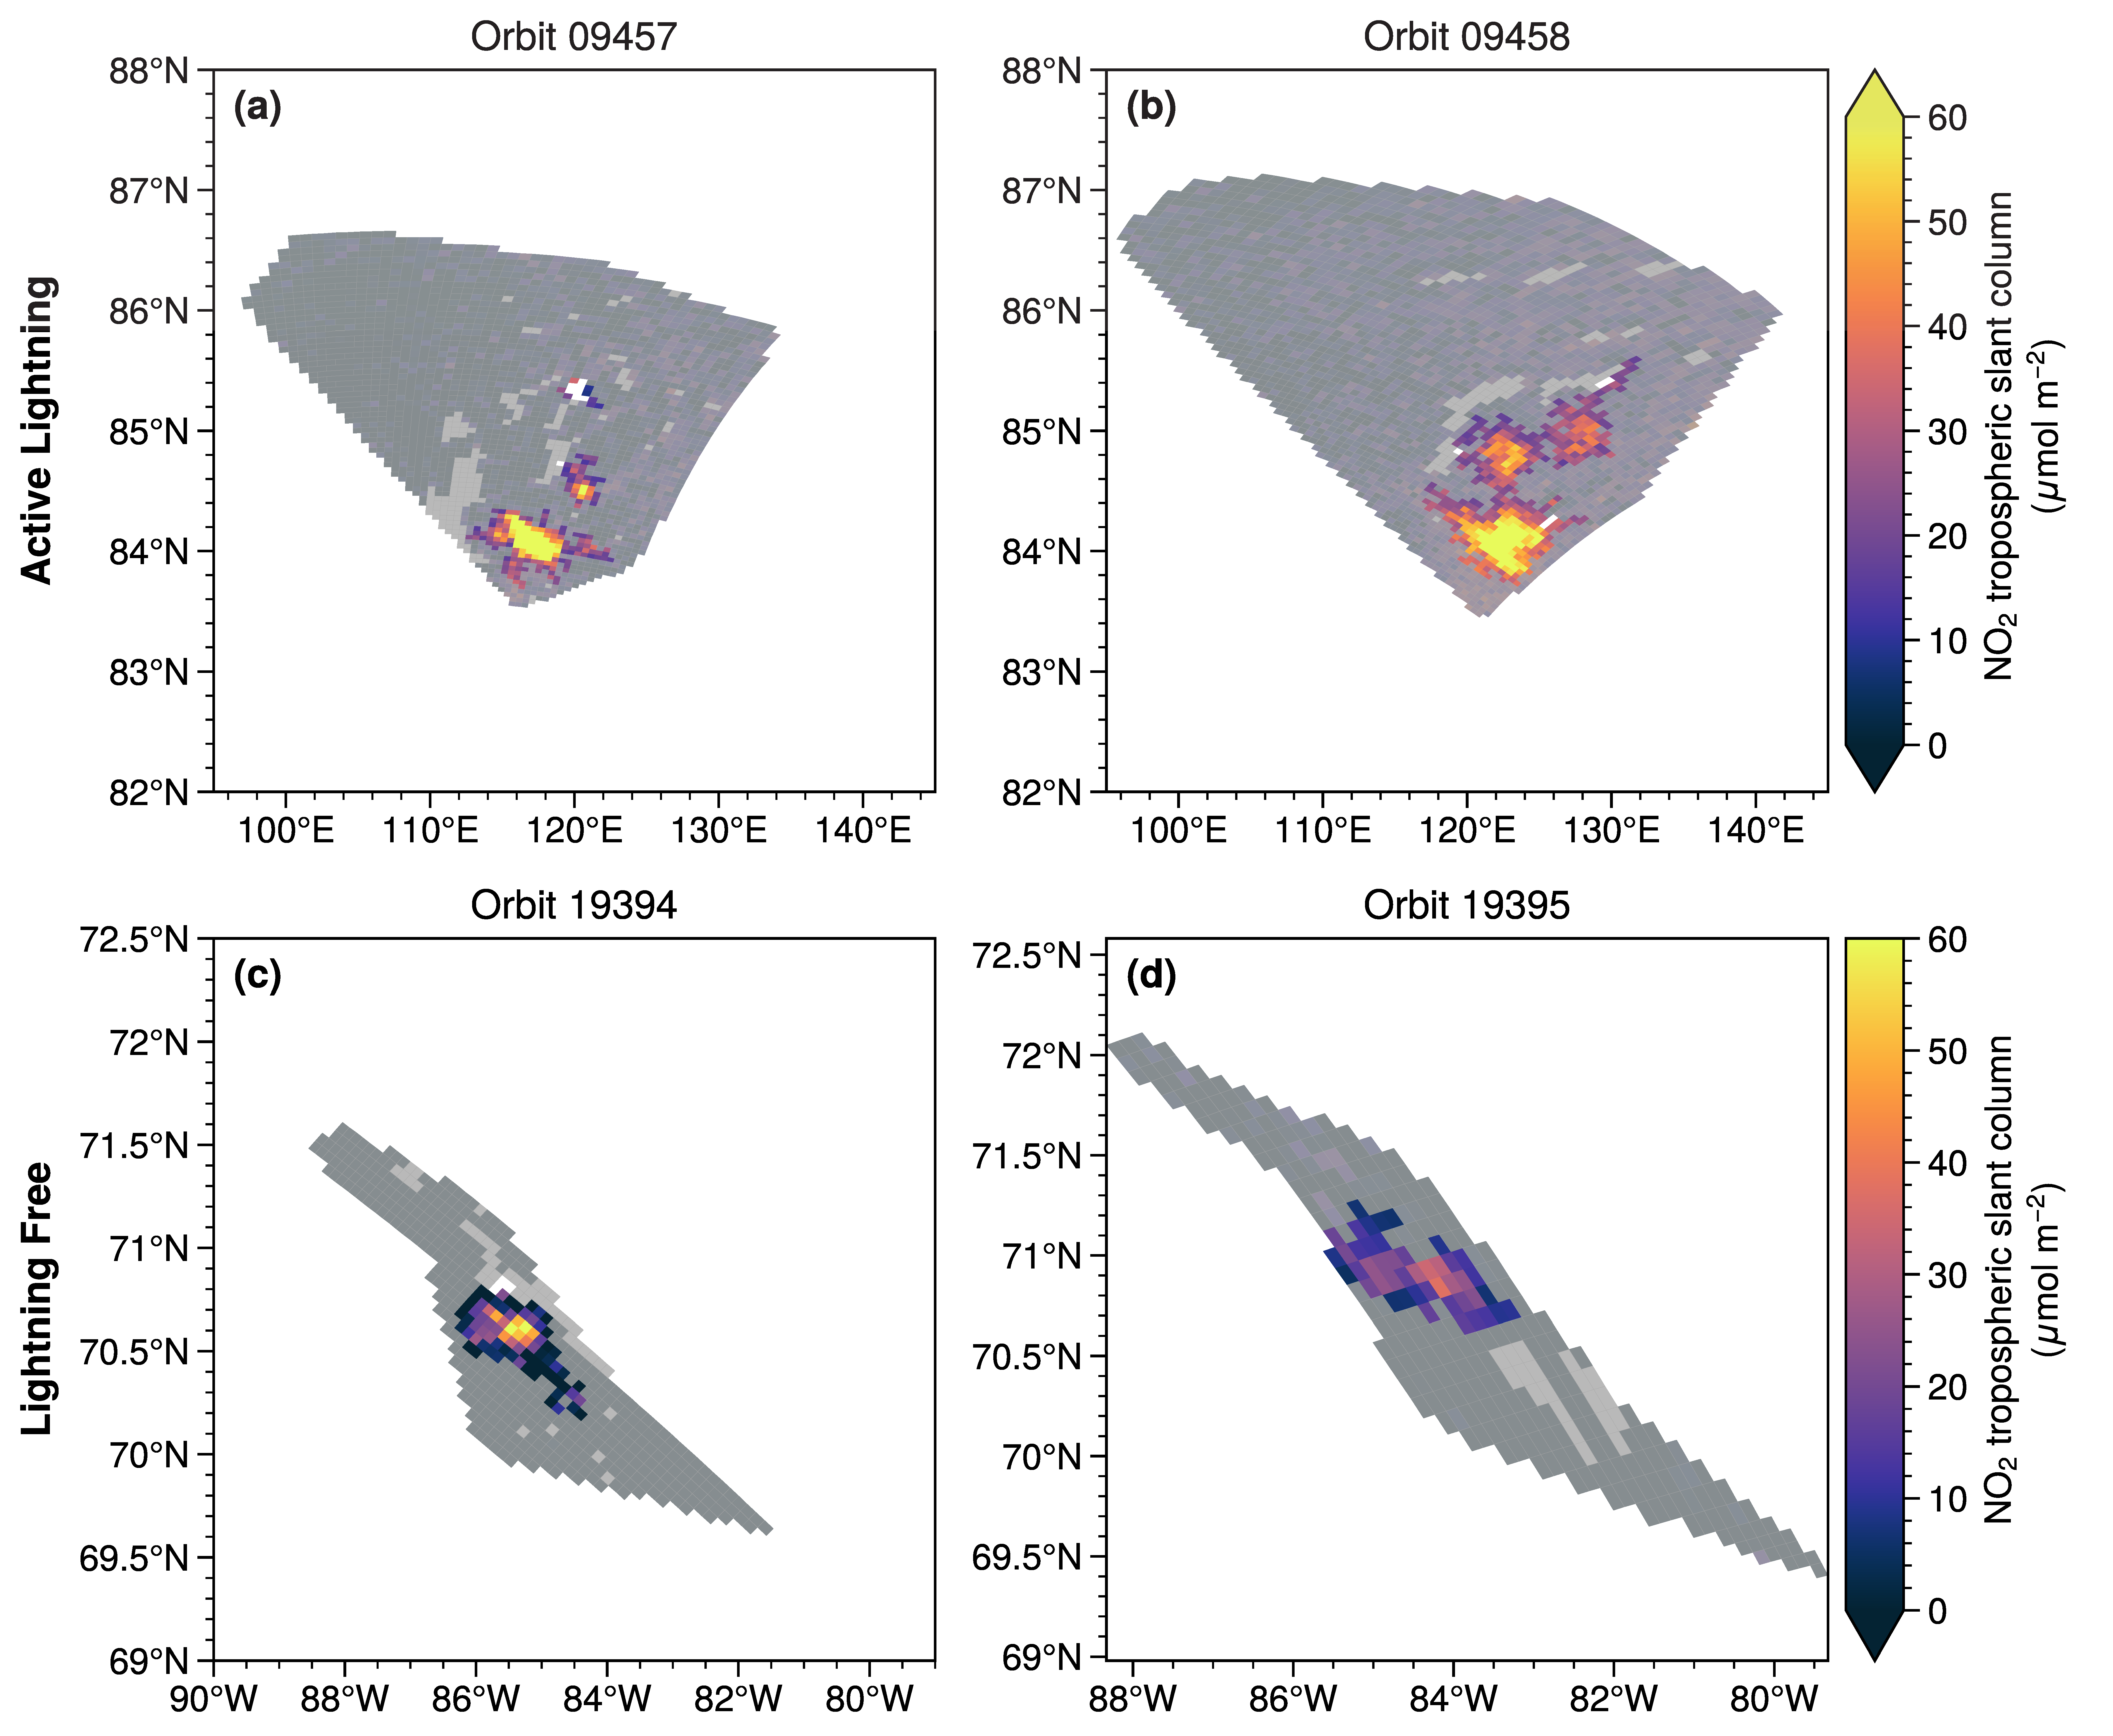
\includegraphics[width=0.85\textwidth]{./figures/arctic_consecutive_orbits.png}
\caption{
受闪电 NO$_2$ 影响的 NO$_2$ 对流层柱浓度的选区(亮色像素)。
(a,b)两次连续的过境数据,且它们之间有活跃的闪电;
(c,d)两次连续的过境数据,但它们之间没有闪电。\\
Figure \ref{fig:consecutive_orbits}.
Selections (bright colored pixels) of NO$_2$ tropospheric columns affected by lightning NO$_2$.
(a--b) Two consecutive orbits with active lightning between them.
(c--d) Two consecutive orbits with no lightning between them.
}
\label{fig:consecutive_orbits}
\end{figure}


在前人的研究中共有三种方法来估算热带和中纬度地区的 LNO$_2$ 产量:

(1) 背景NO$_2$加上LNO$_2$(LNO$_2$$^*$)与闪电之间的线性回归 \citep{Pickering.2016,Allen.2019,Lapierre.2020};

(2) 使用自定义的大气质量因子直接得到LNO$_2$ \citep{Beirle.2009,Zhang.2020b,Zhang.2022a};

(3) 算出LNO$_2$$^*$并减去背景 NO$_2$,其中背景 NO$_2$取自飞机观测 \citep{Pickering.2016,Perez-Invernon.2022} 或未发生闪电的对流像素处的平均NO$_2$ \citep{Bucsela.2019,Bucsela.2010,Allen.2021a}。

由于背景 NO$_2$ 随太阳天顶角而变化,线性回归法不适用于北极地区。
第二种方法需要使用闪电参数化进行详细的 LNO$_2$ 模拟,而目前闪电参数化的不确定性仍非常大\citep{Finney.2018,Romps.2019,Chen.2021a},尤其是在闪电数据集很少的北极地区 \citep{Holzworth.2021}。
因为 TROPOMI 检测到70$^{\circ}$ N 以北的非闪电对流个例有限,
所以最后一种方法需要的平均背景 NO$_2$数据集也不适用于北极地区的网格(即 1 $^{\circ}$ $\times$ 1 $^{\circ}$)。


\begin{table}[H]
\centering
\caption{2019--2021期间得到的闪电 NO$_2$(LNO$_2$)寿命\\
Table \ref{table:lifetime}. Lightning NO$_2$ (LNO$_2$) lifetimes derived from cases (2019--2021).}
\label{table:lifetime}
\footnotesize
{\centering
\begin{tabular}{llllll}
\hline
时间             &         轨道 &    经度 &   纬度 &  $\Delta$面积(\%)$^a$ &  寿命(h)\\
\hline
2019-06-28 00:38 &       08833 &  127.4 &  81.0 &     -14.5 &       3.0 \\
2019-08-14 22:58 &       09513 &  126.0 &  70.4 &       2.0 &       1.7 \\
2020-06-09 19:11 &       13767 &  162.8 &  73.0 &     -43.8 &       3.6 \\
2020-06-15 22:18 &       13854 &  155.6 &  78.7 &      -4.4 &       3.4 \\
2020-07-15 21:19 &       14279 &  109.3 &  75.4 &       4.5 &       2.7 \\
2021-07-11 11:40 &       19395 &  -84.5 &  70.9 &      28.0 &       5.2 \\
\hline
\end{tabular}
\par }
\begin{tablenotes}
\linespread{1}\footnotesize
\item $^a$$\Delta$面积 是 LNO$_2$ 面积在 $T_2$ 时刻相对于 $T_1$ 时刻的百分比变化
($T_1$ 和 $T_2$ 是连续条带的平均过境时间,$T_2$ > $T_1$)。
\item $^a$$\Delta$Area is the percentage change of the LNO$_2$ area at $T_2$ relative to $T_1$
($T_1$ and $T_2$ are the mean overpass time of consecutive swaths, $T_2$ > $T_1$).
\end{tablenotes}
\end{table}

\subsection{闪电氮氧化物的产率}

LNO$_2$ 排放是闪击数和 LNO$_2$ 产率(每次闪击产生的LNO$_2$)的乘积。
然而我们不可能根据来自单次过境的数据直接推导出 LNO$_2$ 产率,
因为 TROPOMI 检测到的 LNO$_2$ 由产生和消耗组成,所以时间维度上需要第二次过境数据。
我们提出可以利用连续轨道的 LNO$_2$ 来估算 LNO$_2$ 产率(见\ref{sec:calc_lnox_pe}节)。
基于对 LNO$_2$ 和闪击的筛选,我们共获得了43个个例,115 个 LNO$_2$ 选区。
其中,60$^{\circ}$ W 和 180$^{\circ}$ W 之间的个例由于 LNO$_2$ 不显著或没有足够的观测值而被剔除。
大多数个例位于 60$^{\circ}$ E 和 180$^{\circ}$ E 之间(图 \ref{fig:arctic_lno2_production}a)。
通过比较闪电分布(图 \ref{fig:arctic_lno2_production}a)与LNO$_2$总和的分布(图 \ref{fig:arctic_lno2_production}b),
我们发现 TROPOMI 观测到的 LNO$_2$ 远离LNO$_2$的排放源。
例如,喀拉海(Kara Sea)没有闪电发生 (77--80$^{\circ}$ N, 65--105$^{\circ}$ E),
但此处的LNO$_2$ 总共约为 5.1 $\times$ 10$^6$ mol。
这是由于对流层上层主导的东风对LNO$_2$的输送作用,从而揭示了匹配闪电和 NO$_2$的重要性。


\begin{table}[H]
\centering
\caption{LNO$_2$产率估算的不确定性$^a$\\
Table \ref{table:arctic_uncertainty}. Uncertainties$^a$ for the estimation of LNO$_2$ production efficiency (PE).}
\label{table:arctic_uncertainty}
\footnotesize
{\centering
\begin{tabular}{llll}
\hline
类型                           &  默认值        & 扰动                 &   不确定度 (\%)  \\
\hline
LNO$_2$ 寿命                   & 3 小时                 & 2 小时和4 小时$^b$      &   36                      \\
IC:CG                         & 1:1                    & 2:1和1:2                  &   33 \\
LNO$_2$ 廓线宽度                & 180 hPa               & 160 hPa 和 200 hPa          &   7   \\
对流层 NO$_2$ 对流层背景浓度      & 第 30 个百分位数        & 第 10 个百分位数$^c$     & 2                \\
LNO$_2$ 选区              & 80\% 置信区间          &  70\% 置信区间   & 13                \\
云压                 & 二级产品               &  $\pm$ 50 hPa$^d$                & 7                \\
其他$^e$       & --                  & --                           &   10                      \\
净不确定度                            &                     &                              &   53                      \\
\hline
\end{tabular}
\par }
\begin{tablenotes}
\linespread{1}\footnotesize
\item $^a$ 不确定度 = (误差$_{\ch{高扰动值}}$ - 误差$_{\ch{低扰动值}}$)/2,
其中 误差$_{\ch{扰动}}$ = (PE$_{\ch{扰动}}$ - PE$_{\ch{默认值}}$)/PE$_{\ch{默认值}}$;
\item $^b$ 基于本研究得到的寿命范围。
\item $^a$ Uncertainty = (Error$_{rising\ perturbed\ value}$ - Error$_{lowering\ perturbed\ value}$)/2
where Error$_{\* perturbed\ value}$ = (PE$_{\* perturbed\ value}$ - PE$_{default\ value}$)/PE$_{default\ value}$.
\item $^b$ Based on the lifetime values calculated in this study.
\item $^c$ \ \citet{Allen.2021a} and \ \citet{Perez-Invernon.2022}.
\item $^d$ \ \citet{VanGeffen.2022}.
\item $^e$ \ \citet{Allen.2021a}.
\end{tablenotes}
\end{table}

尽管如此,LNO$_2$ 与闪击之间仍有一致的空间相关性,因此我们针对每个个例计算其 LNO$_2$ 产率。
研究结果表明,LNO$_2$ 产率在陆地、沿岸和海洋处为 2.0(第 25 至第 75 个百分位数:1.3--3.1)mol每闪击、
3.5(第 25 至第 75 个百分位数:1.1--13.0)mol每闪击
和11.5(第 25 至第 75 个百分位数:1.3--29.9)mol每闪击(图 \ref{fig:arctic_pe_rate}a)。
除了这些中值外,我们还得到了排名前10的LNO$_2$产率,其范围为每次闪击产生27--612 mol NO$_2$(表\ref{table:arctic_pe_lno2}),
这些高值都出现在海洋或沿海地区。
由于个例数量有限,我们无法确定海洋和陆地之间的 LNO$_2$产率是否存在统计学上的显著差异。
但在热带和中纬度地区的研究也表明,由于海洋上的闪电能量更高\citep{Beirle.2014,Hutchins.2013},
海洋上的 LNO$_2$产率是陆地上的两倍\citep{Marais.2018,Allen.2019,Bucsela.2019}。

最近的研究表明,LNO$_2$产率与闪电尺寸有关,尺寸越大,产生的LNO$_2$越多 \citep{Huntrieser.2008,Marais.2018}。
此外,更强的上升气流与更小的闪电和更高的闪电频率相关\citep{Bruning.2013,Bruning.2015,Mecikalski.2015}。
因此,我们计算了闪击率,即单位时间单位LNO$_2$面积内的闪击次数,
它的范围从 2.3$\times$10$^{-10} $m$^{-2}$ h$^{-1}$ 到 4.1$\times$10$^{-6} $m$^{-2 }$ h$^{-1}$,
陆地地区闪击率(6.2$\times$10$^{-7}$ m$^{-2}$ h$^{-1}$)比海洋地区高$\sim$ 11 倍(5.2$\times$10$^{-8}$ m$^{-2}$ h$^{-1}$)。
我们发现闪击率和 LNO$_2$产率之间存在近似的幂律关系(图\ref{fig:arctic_pe_rate}b)。
当闪击率下降2个数量级时,LNO$_2$产率增加10倍,这与中纬度开展的研究一致\citep{Bucsela.2019,Zhang.2020b}。


\begin{figure}[H]
\centering
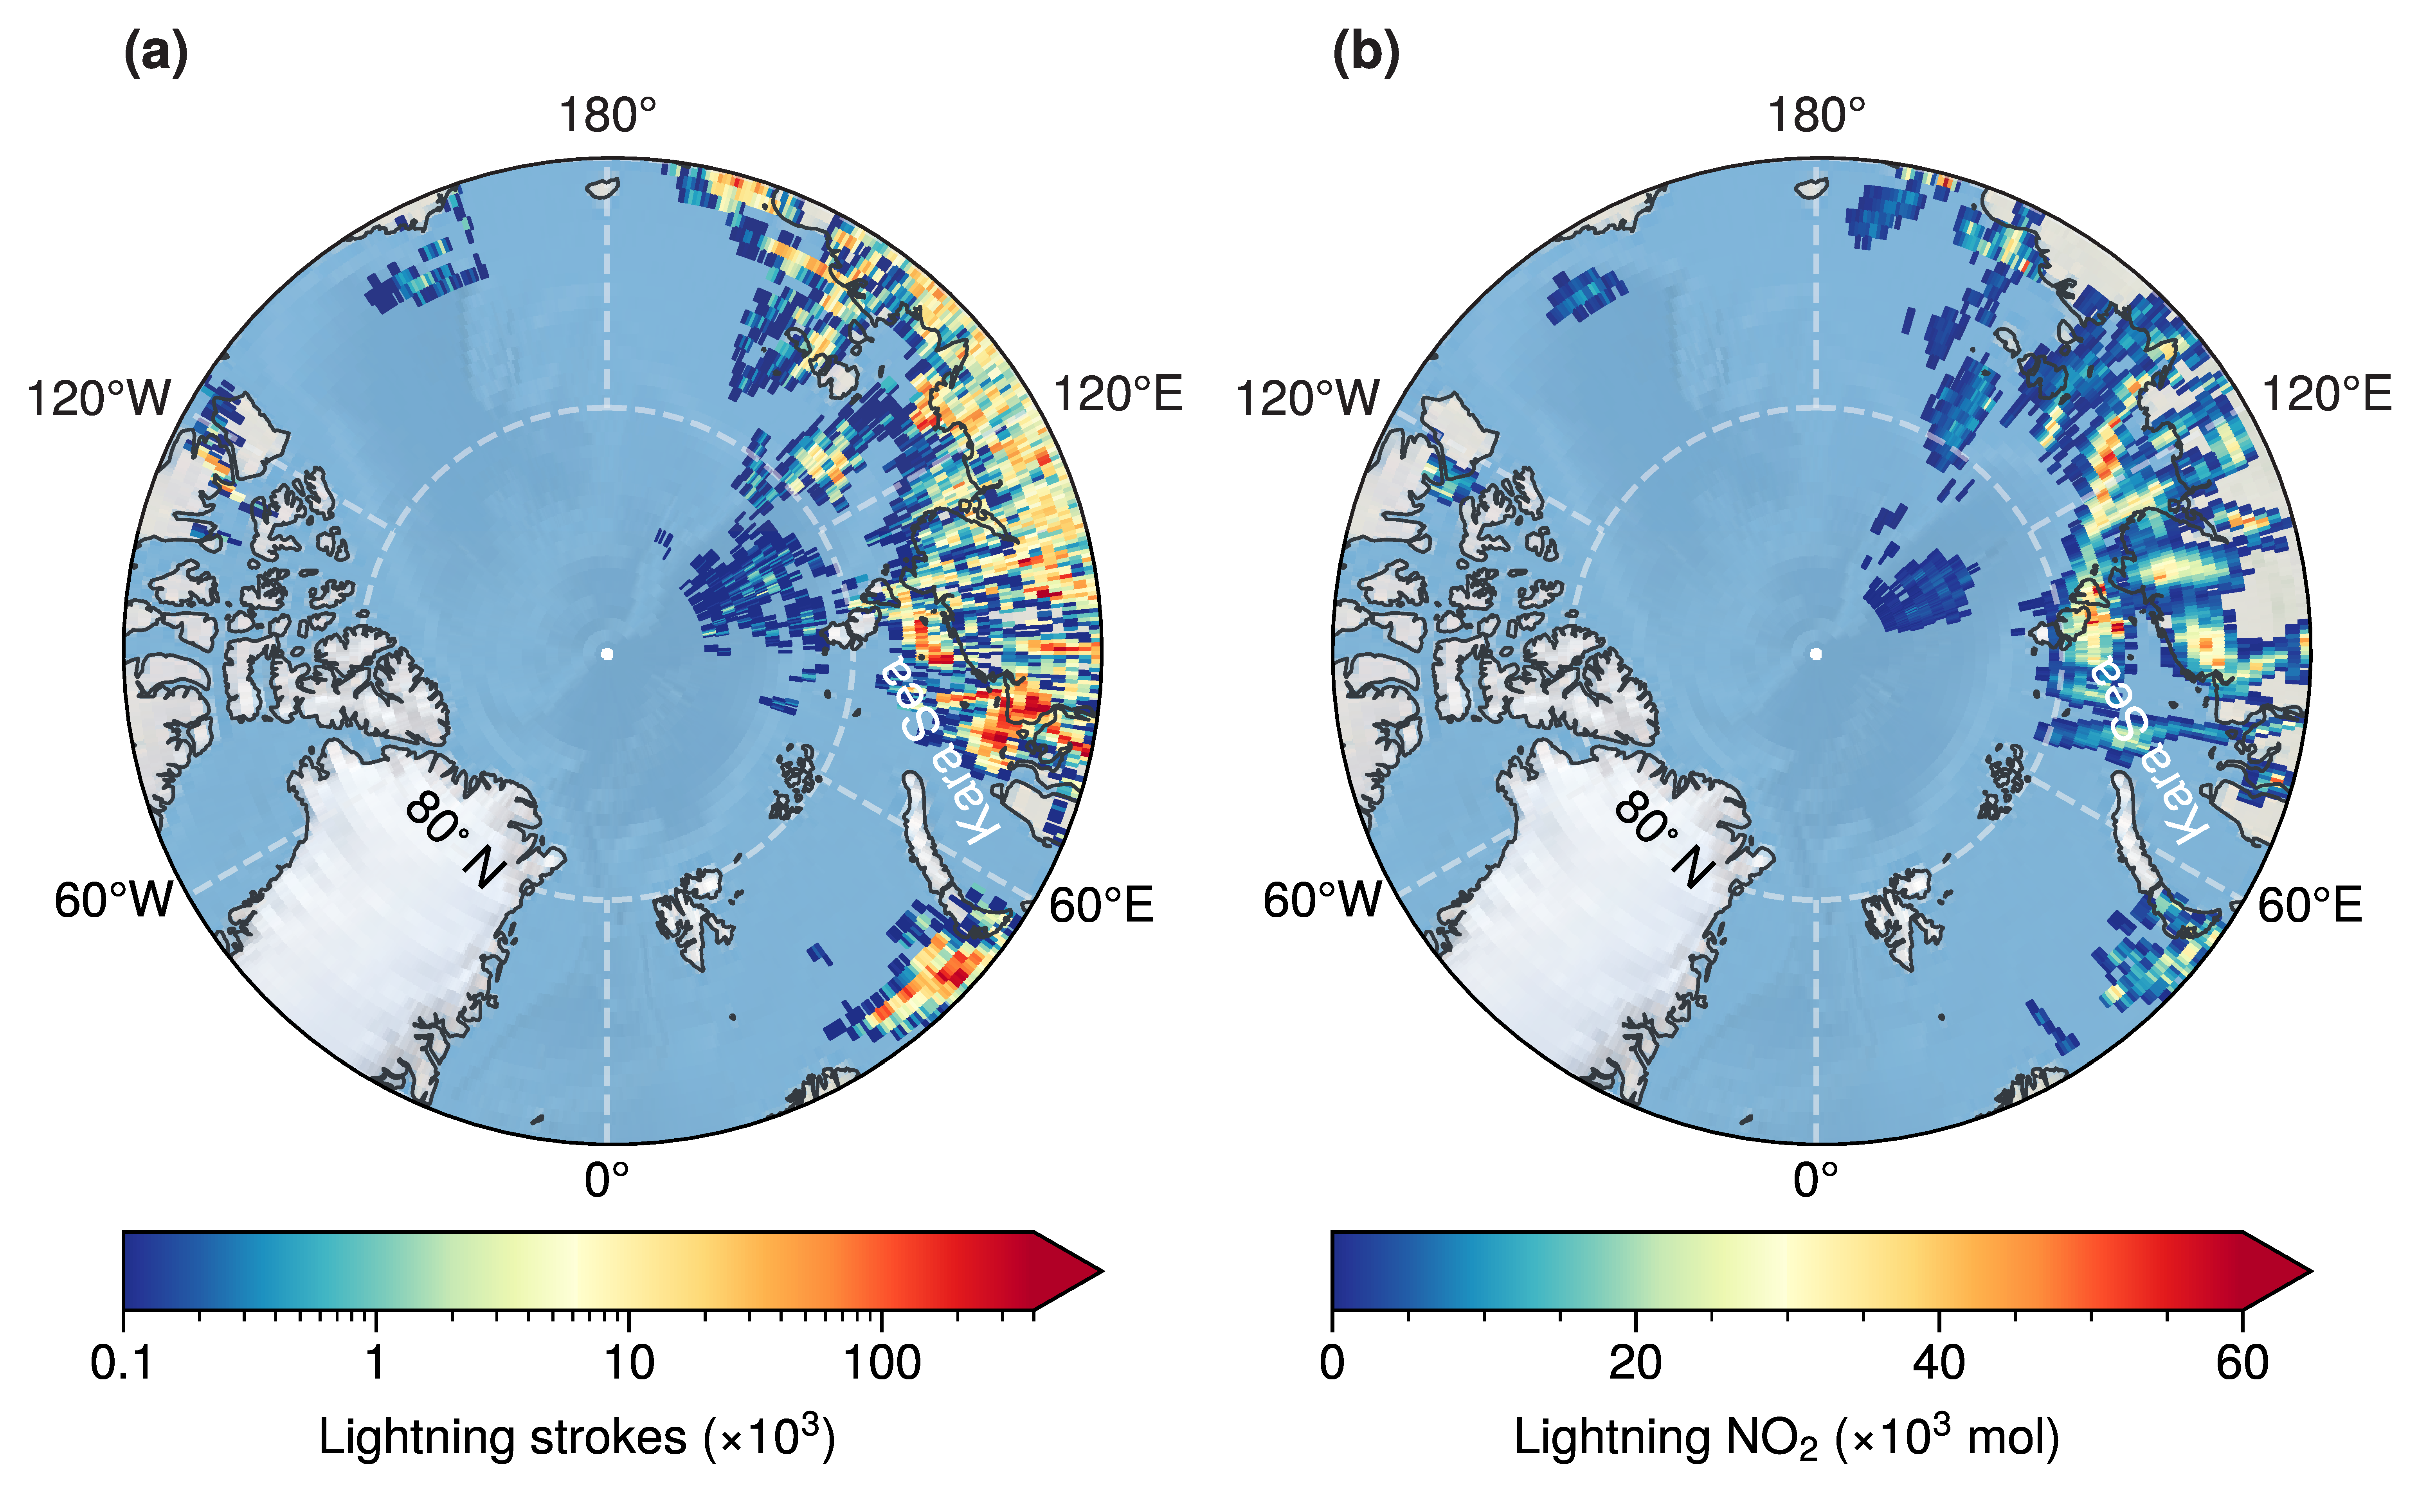
\includegraphics[width=0.85\textwidth]{./figures/arctic_lno2_production.png}
\caption{
(a)每 0.5$^{\circ}$ $\times$ 0.5$^{\circ}$ 网格中所选个例的 GLD360 闪击总和;
(b)每 0.5$^{\circ}$ $\times$ 0.5$^{\circ}$ 网格中由TROPOMI观测数据所得的个例LNO$_2$ 总和。\\
Figure \ref{fig:arctic_lno2_production}. (a) Sum of GLD360 lightning strokes for selected cases per 0.5$^{\circ}$ $\times$ 0.5$^{\circ}$ grid.
(b) Sum of lightning NO$_2$ derived from TROPOMI observations for selected cases per 0.5$^{\circ}$ $\times$ 0.5$^{\circ}$ grid.
}
\label{fig:arctic_lno2_production}
\end{figure}

\begin{table}[H]
\centering
\caption{2019--2021 年10大LNO$_2$产率 \\
Table \ref{table:arctic_pe_lno2}.
Top 10 lightning NO$_2$ (LNO$_2$) production efficiencies from 2019 to 2021.}
\label{table:arctic_pe_lno2}
\footnotesize
{\centering
\begin{tabular}{llllllll}
\hline
时间 &       条带 &   经度 &   纬度 &
区域$^a$ &
闪击数$^b$  & \shortstack{LNO$_2$ 产率 \\ (mol每闪击)} \\
\hline
2020-06-15 20:38 &  13853 &      152.7 &      78.1 &       海洋 &         124 &    611.9 \\
2019-08-11 01:54 &  09458 &      123.5 &      84.5 &       海洋 &         404 &    180.6 \\
2020-07-07 01:51 &  14154 &       53.2 &      72.8 &       沿岸 &        1676 &    151.2 \\
2019-06-26 21:37 &  08817 &      115.4 &      75.7 &       海洋 &        2516 &    144.6 \\
2019-06-20 18:29 &  08730 &      122.2 &      72.8 &       沿岸 &         436 &    105.0 \\
2019-06-20 20:09 &  08731 &      122.1 &      73.1 &       沿岸 &         396 &     81.1 \\
2019-08-11 00:13 &  09457 &      118.0 &      84.2 &       海洋 &        1068 &     51.1 \\
2019-07-11 21:51 &  09030 &      172.4 &      72.2 &       海洋 &         992 &     42.9 \\
2021-07-12 19:44 &  19414 &     -147.6 &      72.7 &       海洋 &        1512 &     32.8 \\
2020-06-16 05:02 &  13858 &      121.3 &      75.8 &       海洋 &         536 &     26.9 \\
\hline
\end{tabular}
\par }
\begin{tablenotes}
\linespread{1}\footnotesize
\item $^a$ 陆地和海洋由50 m Natural Earth数据分类,其中沿岸地区定义为海岸线周围500 m半径。
\item $^b$ 连续轨道间隔期间的总闪击数。
\item $^a$ The land and ocean are classified by the 50 m Natural Earth data, where the coastal region is defined as a 500 m radius around the coastline.
\item $^b$ The total number of strokes during the interval between consecutive orbits.
\end{tablenotes}
\end{table}

\begin{figure}[H]
\centering
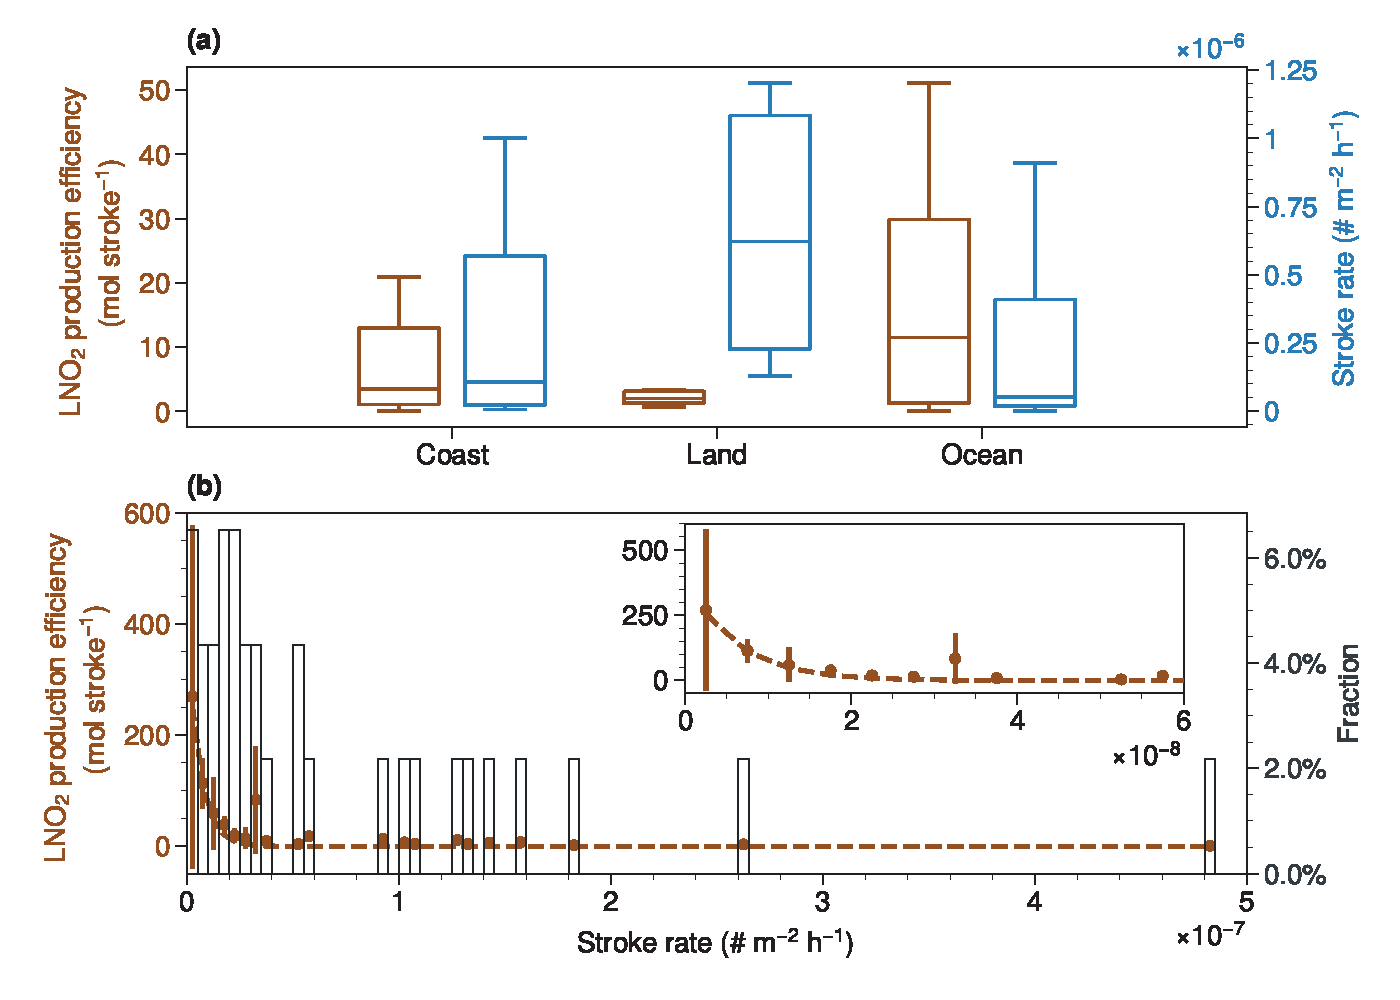
\includegraphics[width=0.85\textwidth]{./figures/arctic_pe_rate.png}
\caption{
(a)三个区域(沿岸、陆地和海洋)的LNO$_2$产率(棕色)和闪击频率(蓝色),
其中沿岸地区为海岸线周围 500 m 的半径。
海岸区域定义为海岸线周围 500 m 半径范围内。
箱线图表示中值,下边界和上边界分别代表第 25 个和第 75 个百分位数,上下误差线分别代表第 10 个和第 90 个百分位数;
(b)LNO$_2$ 产率与闪击频率的关系,叠加每个 5$\times$10$^{-9}$ m$^{-2}$ h$^{-1}$ 中个例占比的直方图。 \\
Figure \ref{fig:arctic_pe_rate}. (a) Comparison of lightning NO$_2$ (LNO$_2$) production efficiency (brown) and stroke rate (blue) for three regions: coast, land, and ocean.
The coast region is defined as a 500 m radius around the coastline.
The box plots indicate the median values; the lower and upper boundaries represent the 25th and 75th percentiles, respectively, and the lower and upper error lines are the 10th and 90th percentiles, respectively.
(b) LNO$_2$ production efficiency vs stroke rate, with histograms of case fractions in each 5$\times$10$^{-9}$ m$^{-2}$ h$^{-1}$ stroke rate bin overlaid.
}
\label{fig:arctic_pe_rate}
\end{figure}


\subsection{氮氧化物的不同排放源贡献}


图 \ref{fig:arctic_no2_comp}a 为2019至2021 年 6--8 月 TROPOMI 在北极观测到的平均 NO$_2$ 柱浓度分布图,
虽然从背景中无法看出LNO$_2$,但在城市、工业和野火地区仍然可以观察到 NO$_2$ 的增强。
例如可以清楚地观察到与阿拉斯加、挪威和俄罗斯的采矿作业相关的 NO$_2$ 柱浓度高值(17 $\pm$ 2 $\mu$mol m$^{-2}$)。
石油和天然气活动也显现出明显的NO$_2$高值,
如加拿大北极麦肯齐谷、北阿拉斯加普拉德霍湾/库帕鲁克和俄罗斯亚马尔天然气管道/乌连戈气田\citep{VanDerA.2020}。
而格陵兰海岸沿线的 NO$_2$ 高值可能是与复杂地形反演相关的错误信号\citep{Hachmeister.2022}。
与 NO$_2$ 污染相反,70$^{\circ}$ N 以北的 TROPOMI 观测显示背景 NO$_2$浓度较低(4.35 $\pm$ 1.26 $\mu$mol m$^{-2}$),
比 60$^{\circ}$ N 和 65$^{\circ}$ N 之间的平均 NO$_2$ 低45\%。

通过将每个个例中LNO$_2$柱浓度的最大值(61 $\pm$ 50 $\mu$mol m$^{-2}$)与北极地区典型的人为和野火 NO$_2$ 进行比较,
我们发现 LNO$_2$ 的柱浓度为其他源的3倍,尽管排放的时间尺度是小时数量级(图 \ref{fig:arctic_no2_comp}b)。
其中发生在拉普捷夫海(Laptev Sea)上空的深对流(图\ref{fig:arctic_large_lno2}),
其LNO$_2$最大值 为 246 $\mu$mol m$^{-2}$,
与美国夏季最高 NO$_2$ 柱浓度相当[234 $\mu$mol m$^{-2}$,\citet{Goldberg.2021a}]。
考虑到LNO$_2$在短时间内的巨大贡献,因此计算北极地区LNO$_2$排放显得十分重要。

\begin{figure}[H]
\centering
\includegraphics[width=0.85\textwidth]{./figures/arctic_no2_comp.png}
\caption{
(a)2019至2021年6--8月当地下午时TROPOMI测得的对流层 NO$_2$ 平均柱浓度(4 km $\times$ 4 km);
(b)四种NO$_2$来源的柱浓度比较:闪电、采矿、石油天然气和野火。
其中闪电NO$_2$浓度为每次对流个例所有像素上NO$_2$的最大值,
而野火、采矿和石油天然气的浓度是(a)中典型位置的每日NO$_2$最大值。
框内的黑线和红线分别是中值和均值,
下边界和上边界分别是第 25 和第 75 个百分位数,
上下误差线分别是第 10 和第 90 个百分位数。\\
Figure \ref{fig:arctic_no2_comp}. (a) Mean 4 km $\times$ 4 km TROPOMI tropospheric NO$_2$ column density in the local afternoon during June--August 2019--2021.
The mining and oil and gas stations are shown as gray and red circles, respectively.
(b) Comparisons of NO$_2$ among four sources: lightning, mining, oil and gas, and wildfire.
The lightning bar represents the maximum NO$_2$ values over pixels for each lightning case,
while the wildfire, mining, and oil and gas bars are the daily maximum NO$_2$ values at typical locations.
The box plots indicate the median (black line) and mean (red line) values; the lower and upper boundaries represent the 25th and 75th percentiles, respectively, and the lower and upper error lines are the 10th and 90th percentiles, respectively.
}
\label{fig:arctic_no2_comp}
\end{figure}

\begin{figure}[H]
\centering
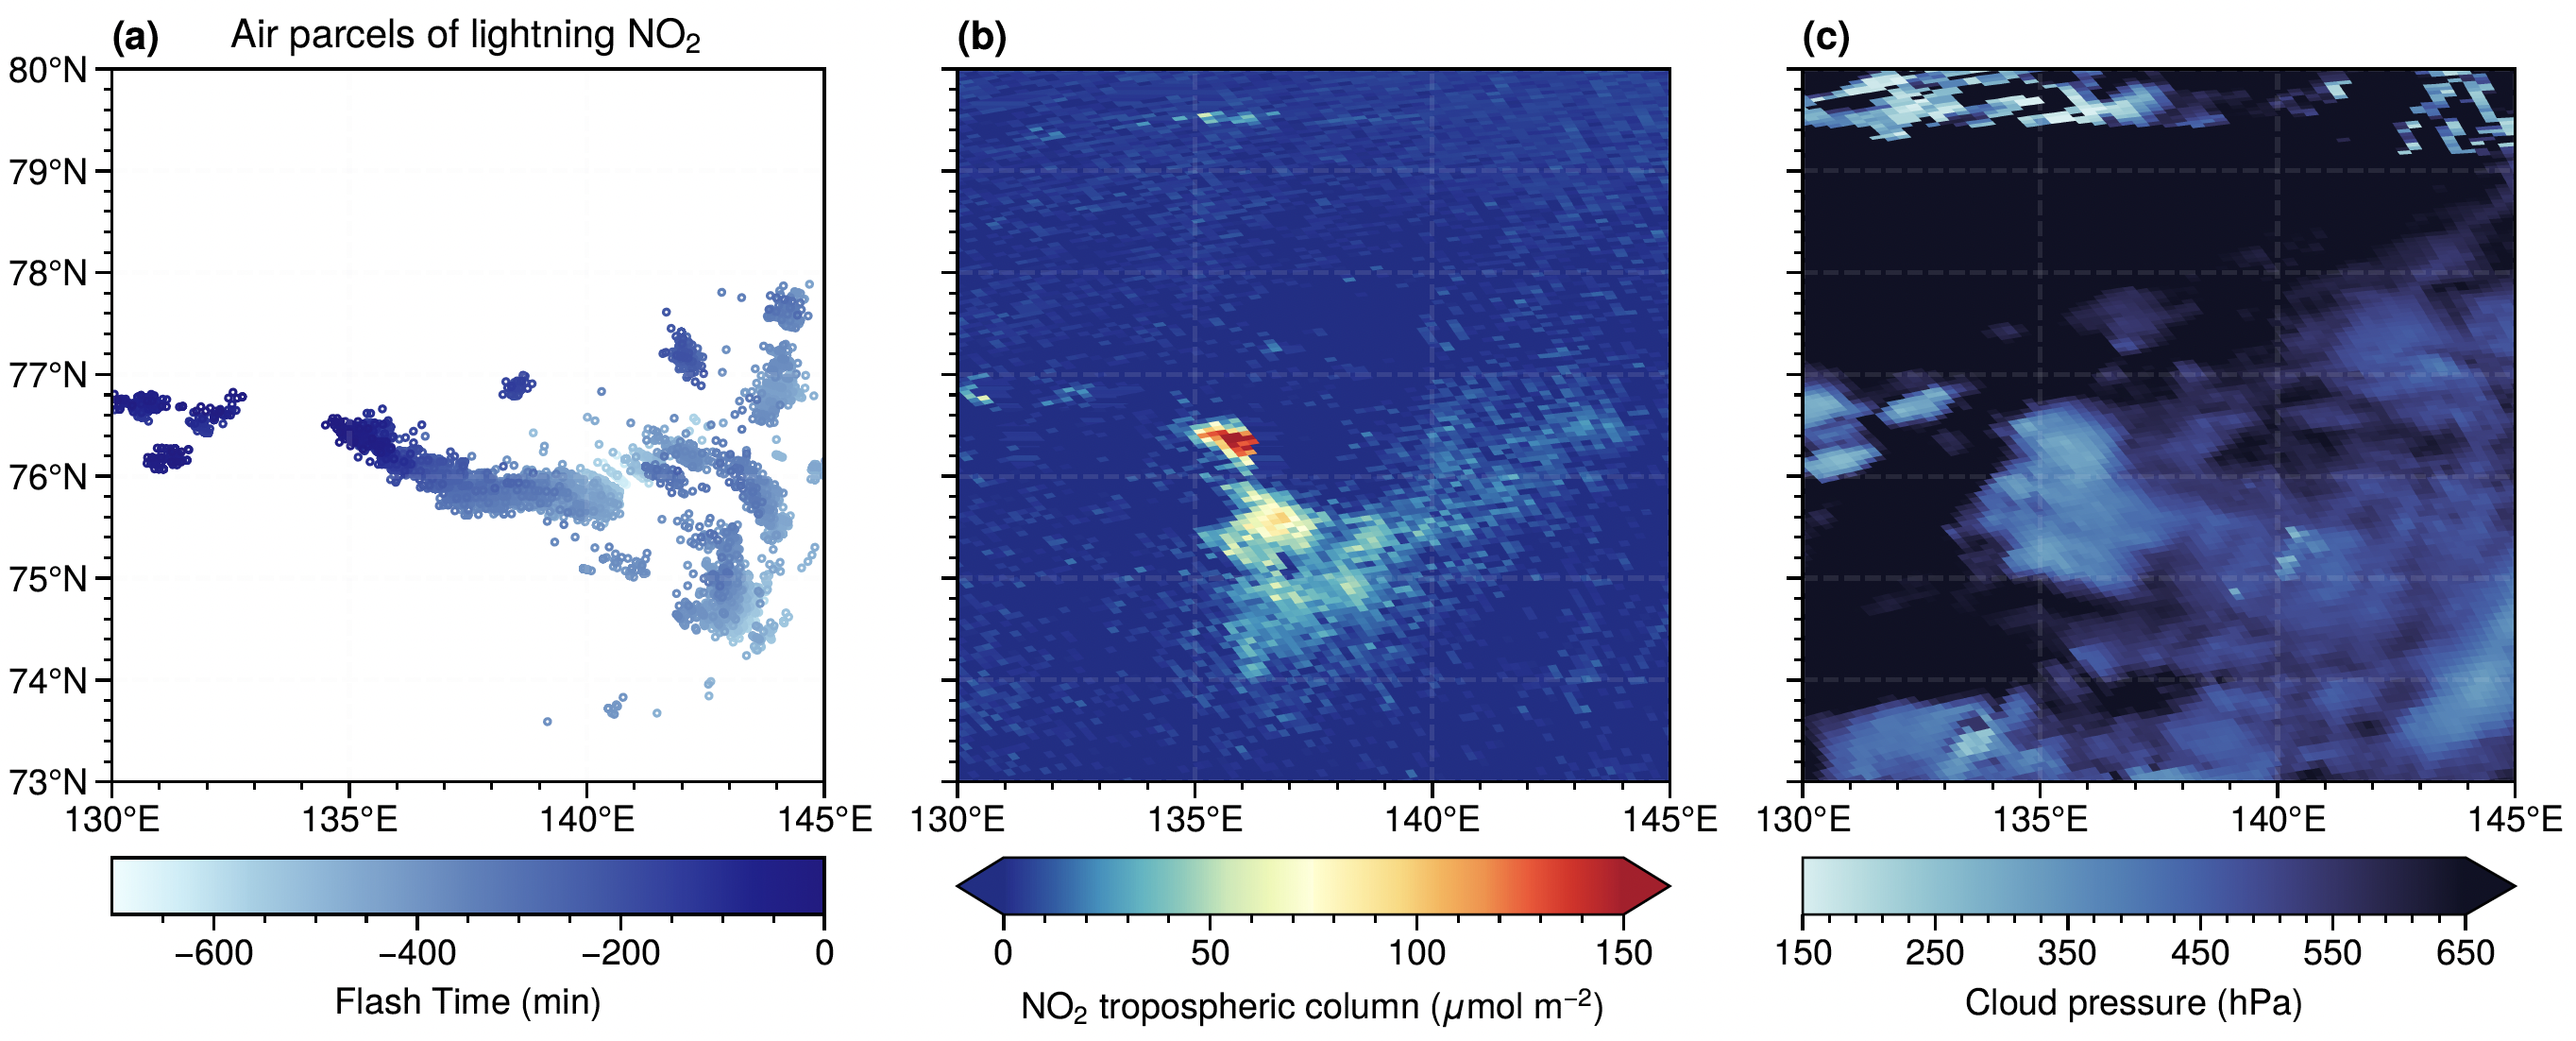
\includegraphics[width=15cm]{./figures/arctic_large_lno2.png}
\caption{
(a)在 500 hPa气压层水平传输的包含闪电 NO$_2$ 的空气块;
(b)TROPOMI 观测到的 NO$_2$ 对流层柱浓度;
(c)TROPOMI 观测到的云压。\\
Figure \ref{fig:arctic_large_lno2}. (a) Transported air parcels containing lightning NO$_2$ at 500 hPa pressure level.
(b) The TROPOMI-detected NO$_2$ tropospheric vertical columns.
(c) The TROPOMI-detected cloud pressures.
}
\label{fig:arctic_large_lno2}
\end{figure}


由于闪击频率计算所用到的面积取决于TROPOMI中LNO$_2$的选区,
我们将闪击数乘以三个地区各自的 LNO$_2$ 产率的中值,并将它们相加作为北极地区LNO$_2$的总排放量($>$ 70$^{\circ}$ N,表\ref{table:arctic_emission})。
结果表明,2020 年 LNO$_2$ 排放量为 109 吨氮,比 2019 年和 2021 年的 LNO$_2$ 平均排放量(83 吨氮)高出 31\%,
位于70$^{\circ}$ N 和 80$^{\circ}$ N 之间增多35\%的排放是其主要贡献。
该区域的2020年平均对流有效位能(CAPE)比2019和2021年的均值高出 32\%
(表\ref{table:arctic_emission} ,图 \ref{fig:arctic_cape_aod})。
而北极点附近(80$^{\circ}$--90$^{\circ}$ N)由于闪电增多,LNO$_2$ 排放量(4.3 吨氮)在 2021 年增加了 353\% (表 \ref{table:arctic_emission})。

假设 NO$_x$ 与 NO$_2$ 的比率为 2.4 \citep{Silvern.2018},计算得到 LNO$_x$ 月排放量为 73 吨氮,
并将其与夏季北极地区的人为和土壤 NO$_x$ 排放量进行比较(图\ref{fig:arctic_emission_comp})。
我们发现土壤月排放总量为 2670 吨氮,是北极陆地上NO$_x$的主要排放源,
而陆地上人为 NO$_x$ 月排放量为350 吨氮与野火月排放量(430 吨氮)在同一量级。
此外船舶月排放总量为 1160 吨氮,是北极海洋上 NO$_x$ 的主要来源,
然而LNO$_x$在北极东北部海洋地区(90--180$^{\circ}$ E, 80--90$^{\circ}$ N)占比高达93\%。
由于对流层上层温度较低,远离雷暴处的NO$_2$寿命为 $\sim$ 0.5--8 天\citep{Schumann.2007,Nault.2017},
故需要更多的研究来评估 LNO$_2$对O$_3$、CO 和 CH$_4$的影响。


本节研究的局限性为LNO$_2$ 产品是在没有反演LNO$_2$垂直廓线的情况下得出的LNO$_2$柱浓度。
虽然云切片技术\citep{BelmonteRivas.2015,Marais.2021}可以从 TROPOMI 观测中推导出 LNO$_2$ 廓线,
但它们需要大样本量来降低噪点。
未来的飞机观测,如深对流云和化学项目[DC3,\citet{Barth.2019}],
可以提供更详细的 LNO$_2$ 廓线,并提高我们对北极地区空气污染和气候变化的理解\citep{Law.2007,Schmale.2018}。


\begin{figure}[H]
\centering
\includegraphics[width=16cm]{./figures/arctic_cape_aod.png}
\caption{
2019至2021年6--8月平均 GLD360 闪击频率、对流有效位能(CAPE,来自 ERA5)和气溶胶光学厚度(550 nm 处的 AOD,来自 MERRA-2)。\\
Figure \ref{fig:arctic_cape_aod}.
Mean GLD360 lightning stroke rate, convective available potential energy (CAPE, from ERA5), and aerosol optical depth (AOD at 550 nm, from MERRA-2) during June--August 2019–-2021.
}
\label{fig:arctic_cape_aod}
\end{figure}


由于预计北极闪电会随着全球变暖而增加,因此准确的闪电观测、模拟和验证对于 LNO$_2$ 的分析非常重要。
由于北极大部分地区被海洋或冰覆盖,地基闪电探测网的探测效率仍然很低\citep{Vagasky.2022}。
此外,北极目前可用的闪电参数化主要集中在陆地,尤其是永冻区\citep{Chen.2021a}。
因此,一致的卫星观测(例如 OTD)对于北极闪电研究至关重要。
虽然热带降雨测量任务[TRMM,\citet{Cecil.2014}]和国际空间站[ISS,\citet{Blakeslee.2020}]上都配备了闪电成像传感器(LIS)
但是它们只探测热带和中纬度闪电。
其中TRMM LIS 覆盖低纬度($\pm$ 38$^{\circ}$),ISS LIS 的覆盖范围扩展到更高纬度($\pm$ 55$^{\circ}$)。
未来计划中的闪电传感器可以探测的纬度范围目前尚不清楚。
然而将水文气象卫星[例如 Arktika-M,\citet{Asmus.2021}]
与闪电传感器[例如全球闪电测绘仪(GLM)和闪电测绘成像仪(LMI),\citet{Goodman.2013,Yang.2017}] 相结合,可以帮助我们更好地了解北极闪电的变化。


\begin{figure}[H]
\centering

\includegraphics[width=0.95\textwidth]{./figures/arctic_emission_comp.png}
\caption{
北极地区6--8月的NO$_x$月排放量
(a)人为排放(包括船舶排放);(b)土壤排放;
(c)船舶排放。
闪电 NO$_x$ 排放是 2019 年至 2021 年的平均值。
其他排放来自哥白尼大气监测服务(CAMS)2018 年全球排放清单。\\
Figure \ref{fig:arctic_emission_comp}. Monthly NO$_x$ emissions in the Arctic from June to August.
(a) Anthropogenic emissions including ship emissions, (b) soil emissions, and (c) lightning emissions.
The lightning NO$_x$ emissions are the mean values from 2019 to 2021, while the other emissions are from the 2018 Copernicus Atmosphere Monitoring Service (CAMS) global emission inventories.
}
\label{fig:arctic_emission_comp}
\end{figure}


\section{污染地区(美国大陆)} \label{sec:us}

\subsection{模式设置} \label{sec:model_settings_us}

如\ref{sec:amf_definition}节所述,污染地区LNO$_2$柱浓度的估算
需要同时考虑详细的LNO$_2$和人为污染NO$_2$的分布,
因此针对美国大陆(本节)和中国东南部(\ref{sec:china}节)的研究使用WRF-Chem高分辨率模式来获得AMF,进而计算LNO$_2$的柱浓度。
在美国大陆的模拟研究中使用的WRF-Chem版本为3.5.1,水平网格大小为12 km $\times$ 12 km (图\ref{fig:us_domain}a),垂直层数为29层,时间步长为72 s。
气象条件的初始场和边界场为时间分辨率3小时的北美区域再分析(NARR)数据集,
每3小时应用一次边界条件和四维数据分析(FDDA)逼近,
其中温度、水汽和水平风以0.0003 s$^{-1}$ 的系数逼近\citep{Laughner.2017}。
微物理过程采用Lin方案\citep{Lin.1983},积云参数化为Grell 3D方案\citep{Grell.1993a,Grell.2002a},
长波辐射采用RRTM方案\citep{Iacono.2008},短波辐射采用Goddard方案,
陆面过程使用Noah陆面模式\citep{Koren.1999},边界层采用YSU方案\citep{Hong.2006}。
闪电参数化采用基于对流参数化的中性浮力水平\citep{Pickering.1992},云闪与地闪的比例基于\citet{Boccippio.2001}.

\begin{figure}[H]
\centering
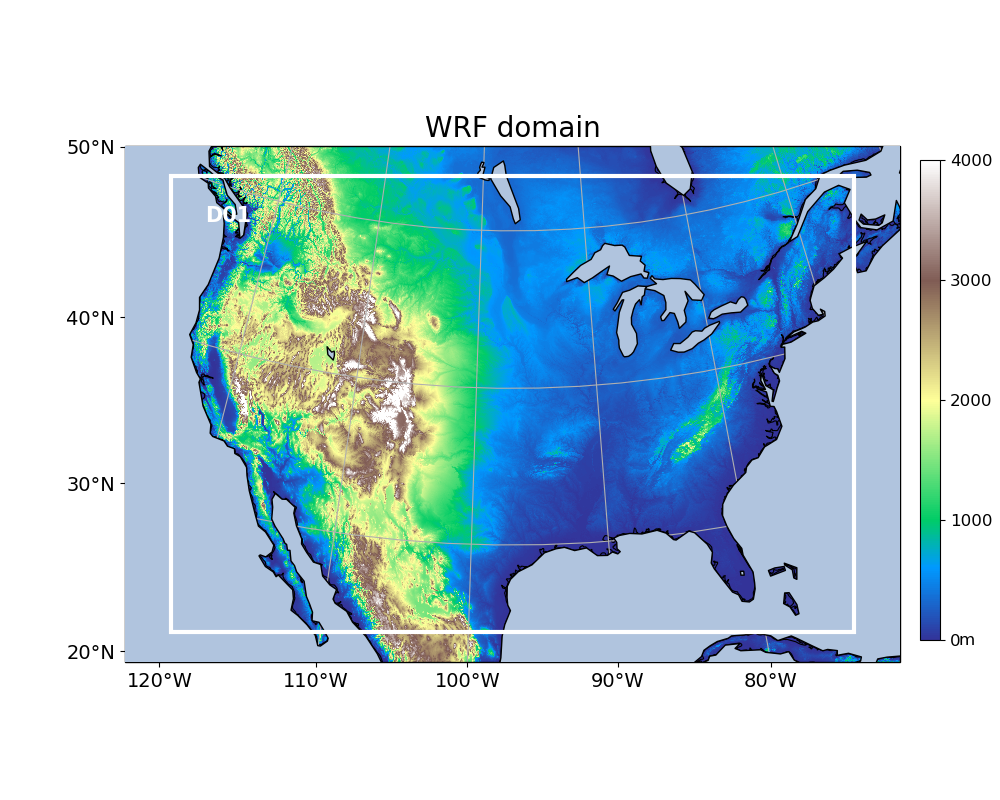
\includegraphics[width=11cm]{./figures/us_domain.png}
\caption{WRF-Chem 模拟区域和地形高度(m),网格数为 350 $\times$ 290,水平分辨率为 12 km。 \\
Figure \ref{fig:us_domain}. Domain and terrain height (m) of the WRF-Chem simulation with 350 x 290 grid cells and a horizontal resolution of 12 km.}
\label{fig:us_domain}
\end{figure}

化学的初始场和边界场采用臭氧和相关化学示踪剂模式第4版[MOZART-4,\citet{Emmons.2010}]的输出场。
人为排放由2011年美国国家排放清单(NEI)驱动,并根据环境保护署年度总排放量,按模拟的年份进行调整\citep{EPA.2015}。
生物排放使用MEGAN源,化学机制是区域大气化学机制第2版[RACM2,\citet{Goliff.2013}],
并由\citet{Browne.2014}和\citet{Schwantes.2015}进行了更新。
此外,LNO$_x$参数化采用每次闪电产生200 mol NO,调整因子为1,以下简称“1$\times$200 mol NO每闪电”。
WRF-Chem中LNO的垂直分布采用基于\citet{Ott.2010}的双峰型闪电NO(LNO)廓线\citep{Laughner.2017},
LNO和LNO$_2$廓线是指开启和关闭LNO排放的模拟之间各自垂直廓线的差异。


\subsection{闪电氮氧化物的筛选条件}

首先我们使用恒定值网格化法,将公式(\ref{eq:AMF_LNO2})所得的LNO$_x$垂直柱浓度(V$_{\ch{LNO_x}}$)分配至0.05$^{\circ}$ $\times$ 0.05$^{\circ}$网格\citep{Kuhlmann.2014}。
接着在 1$^{\circ}$ $\times$ 1$^{\circ}$的网格中进行分析,要求每个网格至少有50个有效的0.05$^{\circ}$ $\times$ 0.05$^{\circ}$网格数据,从而最小化噪点数据。
具体筛选条件和主要计算步骤如下。

云辐射分数(CRF,CRF $\geq$ 70\%,CRF $\geq$ 90\%,CRF = 100\%)和 云压(CP,CP $\leq$ 650 hPa)
通常是判断OMI像素是否包含深对流云的标准\citep{Ziemke.2009,Choi.2014,Pickering.2016}。
% 不同CRF对LNO$_x$产品的影响将在\ref{subsec:retrieval_polluted}节探讨。
此外,我们将另一个云分数 (CF)标准应用于 WRF-Chem 的模拟结果,以确保成功模拟出对流。
具体而言,CF是由 Xu-Randall 方法计算的 350--400 hPa 之间的最大云分数\citep{Xu.1996,Strode.2017}。
我们根据\citet{Strode.2017}的建议,选择350--400 hPa的CF $\geq$ 40\%来判断模拟所处的网格是多云或晴空,
可避免模拟高云中的偏差。

除了云特性之外,OMI能探测到新生LNO$_x$的另一条件为一段时间内有足够的闪电或闪击。
其中,时间窗口 (t$_{window}$) 是 OMI 过境之前的时间段。
\citet{Lapierre.2020}利用1$^{\circ}$ $\times$ 1$^{\circ}$网格的对角线长度和OMI过境时美国大陆上空500--100 hPa的平均风速计算得到t$_{window}$为2.4 h。
同时,\citet{Lapierre.2020}定义在t$_{window}$时间段内至少发生2400次闪电或8160次闪击的网格,才能提供足够的LNO$_x$给OMI探测。
\citet{Bucsela.2019}的研究表明,低频率的闪电具有更高的LNO$_x$产率,而该段数据在\citet{Lapierre.2020}研究中被剔除。
通过比较使用每个网格至少2400次闪电和至少1次闪电的标准所得结果,我们也得到相同的结论(图\ref{fig:us_flash_threshold})。
由于我们的研究重点是开发一种新的AMF,并将计算结果与使用类似闪电阈值的其他产品进行比较\citep{Pickering.2016,Lapierre.2020},
因此我们接下来使用相同的“至少2400次闪电”标准来进行结果分析。


\begin{figure}[H]
\centering
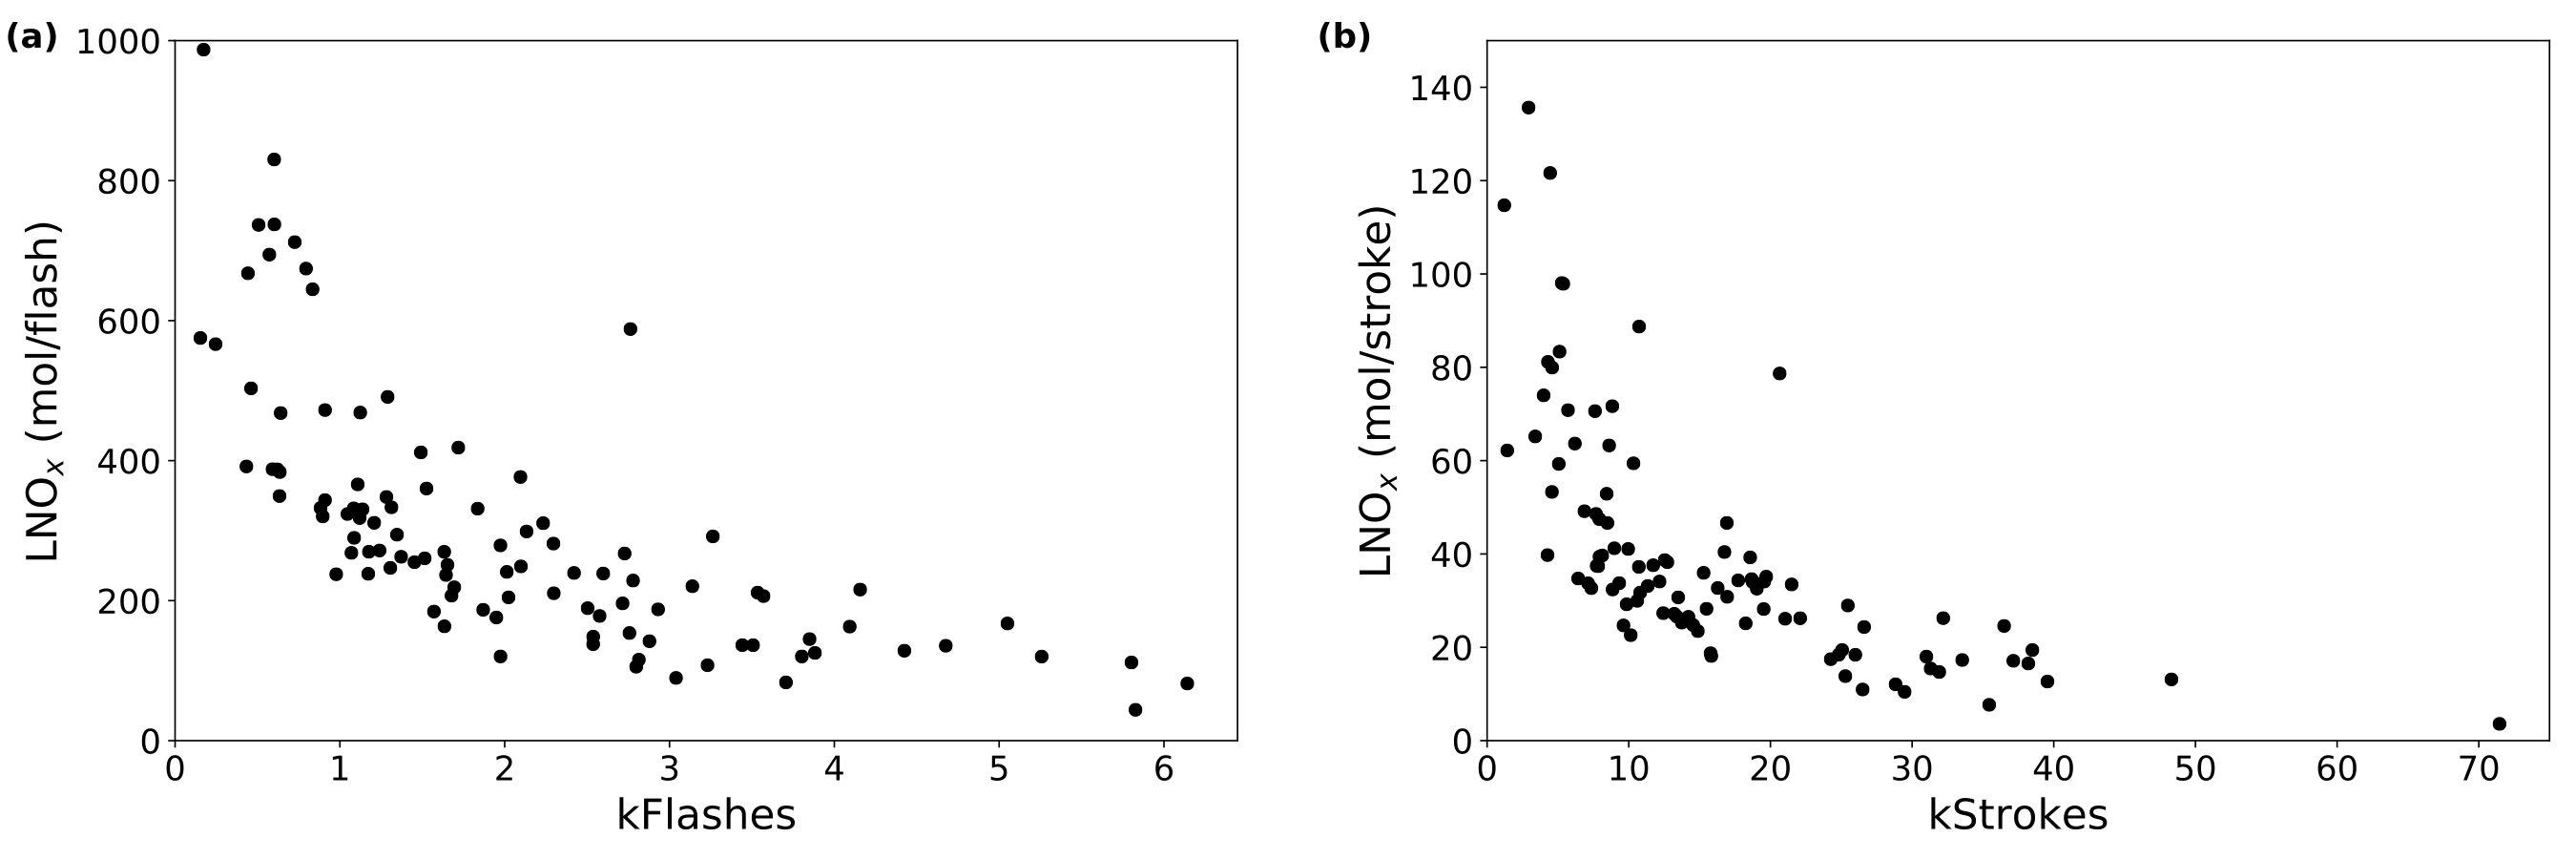
\includegraphics[width=0.9\textwidth]{./figures/us_flash_threshold.png}
\caption{
(a) 每日 LNO$_x$ 产率与 ENTLN 总闪的关系,筛选条件为CRF $\geq$ 90\% 且1$^{\circ}$ $\times$ 1$^{\circ}$网格中至少有1次闪电;
 (b) 与 (a) 相同,但针对闪击。\\
Figure \ref{fig:us_flash_threshold}. (a) Daily LNO$_x$ production efficiencies versus ENTLN total flashes data, with CRF $\geq$ 90\% and a flash threshold of 1 flash box$^{-1}$.
(b) Same as (a) but for strokes.}
\label{fig:us_flash_threshold}
\end{figure}


为确保WRF-Chem成功模拟出闪电,并考虑到闪电参数化的不确定性,我们将每个1$^{\circ}$ $\times$ 1$^{\circ}$网格模拟的总闪电(TL)阈值设置为1000,该阈值低于ENTLN闪电观测使用的阈值。
针对除LNO$_2$之外的其他NO$_2$源,我们定义了模拟的云上闪电NO$_2$柱浓度($V_{\ch{LNO2Vis}}$)
与云上NO$_2$柱浓度($V_{\ch{NO2Vis}}$)之比,来判断OMI是否可以检测到足够的LNO$_2$,
若该比值$\geq$50\%,则表明云层上方超过一半的NO$_x$具有LNO$_x$源。
此外还需考虑氧化有关的NO$_2$寿命,
\citet{Nault.2017}的研究表明NO$_2$在对流附近的寿命($\tau$)为$\approx$3 h,故NO$_2$的初始值可由式(\ref{eq:inition})求解。

\begin{equation} \label{eq:inition}
NO_2(0) = NO_2(\mathrm{OMI})\ e^{0.5t/\tau}
\end{equation}

其中$NO_2(0)$是在时间 t=0 时刻排放的NO$_2$摩尔数,$NO_2(\mathrm{OMI})$是在 OMI 过境时间测得的NO$_2$摩尔数,
0.5t是穿过网格的时间即1.2 h(假设闪电出现在每个1$^{\circ}$ $\times$ 1$^{\circ}$网格的中心)。
每个网格的V$_{\ch{LNO_x}}$为网格中所有0.05$^{\circ}$ $\times$ 0.05$^{\circ}$像素的V$_{\ch{LNO_x}}$平均值,
然后乘以网格的面积得到LNO$_x$摩尔数。
最后,有两种方法可用于估算季节性平均LNO$_2$每闪电、LNO$_x$每闪电、LNO$_x$每闪击和 LNO$_x$每闪击:

(1)求和法,将LNO$_x$的总和除以5--8月中每个1$^{\circ}$ $\times$ 1$^{\circ}$网格里发生的闪电或闪击总数;

(2)线性回归方法,将线性回归应用于每日LNO$_x$和闪电或闪击平均值。

% \subsection{适合反演闪电氮氧化物的条件} \label{subsec:criteria}

根据以上条件,我们定义了六种不同的筛选条件组合(表\ref{table:Abbreviations}),并将线性回归法应用于原始数据。

\begin{table}[H]
\caption{本研究中使用的标准的缩写定义\\Table \ref{table:Abbreviations}. Definitions of the abbreviations for the criteria used in this study.}
\scriptsize
\begin{tabular}{ll}
\hline
缩写$^a$ & 全称 [来源] \\
\hline
CRF                             & 云辐射分数 Cloud radiance fraction [OMI] \\
CP                              & 云压Cloud pressure [OMI] \\
CF                              & 云分数 Cloud fraction [WRF-Chem] \\
TL                              & 总闪电数 Total lightning flashes [WRF-Chem] \\
ratio                           & $V_{\ch{LNO2Vis}}$ / $V_{\ch{NO2Vis}}$ [WRF-Chem] \\
CRF$\alpha$\_ENTLN                   & CRF $\geq$ $\alpha$ + ENTLN 闪电(闪击)$\geq$ 2400(8160)[ENTLN]\\
CRF$\alpha$\_CF40\_ENTLN              & CRF $\geq$ $\alpha$ + ENTLN 闪电(闪击)$\geq$ 2400(8160)+ CF $\geq$ 40\% \\
CRF$\alpha$\_ENTLN\_TL1000            & CRF $\geq$ $\alpha$ + ENTLN 闪电(闪击)$\geq$ 2400(8160)+ TL $\geq$ 1000 \\
CRF$\alpha$\_CF40\_ENTLN\_TL1000      & CRF $\geq$ $\alpha$ + ENTLN 闪电(闪击)$\geq$ 2400(8160)+ CF $\geq$ 40\% + TL $\geq$ 1000 \\
CRF$\alpha$\_ENTLN\_TL1000\_ratio50   & CRF $\geq$ $\alpha$ + ENTLN 闪电(闪击)$\geq$ 2400(8160)+ TL $\geq$ 1000 + ratio $\geq$ 50\% \\
CRF$\alpha$\_CF40\_ENTLN\_TL1000\_ratio50 & CRF $\geq$ $\alpha$ + ENTLN 闪电(闪击)$\geq$ 2400(8160)+ CF $\geq$ 40\% + TL $\geq$ 1000 + ratio $\geq$ 50\% \\
CRF$\alpha$\_ENTLN1(3.4)\_TL1\_ratio50    & CRF $\geq$ $\alpha$ + ENTLN 闪电(闪击)$\geq$ 1(3.4)+ TL $\geq$ 1 + ratio $\geq$ 50\% \\
\hline
\end{tabular}
\begin{tablenotes}
\linespread{1}\footnotesize
\item $^a$ $\alpha$有三种选择:70\%、90\%以及100\%。
\item $^a$ $\alpha$ has three options: 70\%, 90\% and 100\%.
\end{tablenotes}
\label{table:Abbreviations}
\end{table}


在CRF90\_ENTLN条件下,有效闪电(闪击)数据对应共有99(102)天。
以闪电类ENTLN数据为例,在 CRF90\_ENTLN\_TL1000\_ratio50 条件下,有效天数从 99 减少至 81,而LNO$_x$产率从 52.1 $\pm$ 51.1 mol每闪电增加到 54.5 $\pm$ 48.1 mol每闪电。
该结果与 CRF90\_ENTLN\_TL1000 条件下所得的结果几乎相同。
尽管这表明TL筛选条件已足够严格,但最好包括云上LNO$_2$占比的筛选条件,以防不同的AMF方法中存在一些例外情况。
由于 CF $\geq$ 40\% 会导致有效数据和产率急剧下降,因此我们仅仅使用 CRF 对数据进行筛选。
最后,我们选择至少2400次闪电或至少8160次闪击、TL $\geq$ 1000 和云上LNO$_2$占比 $\geq$ 50\% 作为阈值,来探索三种不同 CRF 条件(CRF $\geq$ 70\%、CRF $\geq$ 90\% 和 CRF = 100\%)对 LNO$_x$ 估算产生的影响(表\ref{table:CRFs})。


\begin{table}[H]
\caption{根据表\ref{table:Abbreviations}中的定义得到的LNO$_x$产率\\Table \ref{table:conditions} LNO$_x$ production efficiencies for different combinations of criteria defined in Table \ref{table:Abbreviations}.}
\scriptsize
\begin{tabular}{lccccc}
\hline
条件$^a$ & ENTLN类型$^b$ & LNO$_x$每闪电 or LNO$_x$每闪击 & R值 & 截距 (10$^{6}$mol) & 天数$^c$ \\
\hline
CRF90\_ENTLN                        & 闪电  & 52.1 $\pm$ 51.1 & 0.20 & 0.21  & 99 \\
CRF90\_CF40\_ENTLN                  & 闪电  & 84.2 $\pm$ 31.5 & 0.54 & -0.04 & 70 \\
CRF90\_ENTLN\_TL1000                & 闪电  & 61.9 $\pm$ 49.1 & 0.27 & 0.33  & 83 \\
CRF90\_CF40\_ENTLN\_TL1000          & 闪电  & 63.4 $\pm$ 52.9 & 0.38 & 0.26  & 38 \\
CRF90\_ENTLN\_TL1000\_ratio50       & 闪电  & 54.5 $\pm$ 48.1 & 0.25 & 0.39  & 81 \\
CRF90\_CF40\_ENTLN\_TL1000\_ratio50 & 闪电  & 90.0 $\pm$ 65.0 & 0.46 & 0.15  & 32 \\
CRF90\_ENTLN                        & 闪击 & 6.7 $\pm$ 4.1 & 0.31 & 0.23  & 102 \\
CRF90\_CF40\_ENTLN                  & 闪击 & 10.3 $\pm$ 3.6 & 0.55 & 0.08 & 79 \\
CRF90\_ENTLN\_TL1000                & 闪击 & 7.5 $\pm$ 5.1 & 0.29 & 0.38  & 94 \\
CRF90\_CF40\_ENTLN\_TL1000          & 闪击 & 8.6 $\pm$ 6.2 & 0.39 & 0.27  & 46 \\
CRF90\_ENTLN\_TL1000\_ratio50       & 闪击 & 7.0 $\pm$ 4.8 & 0.29 & 0.42  & 93 \\
CRF90\_CF40\_ENTLN\_TL1000\_ratio50 & 闪击 & 8.9 $\pm$ 7.0 & 0.39 & 0.31  & 40 \\
\hline
\label{table:conditions}
\end{tabular}
\begin{tablenotes}
\linespread{1}\footnotesize
\item $^a$ 定义见表\ref{table:Abbreviations}。
\item $^b$ ENTLN阈值为OMI过境前2.4小时内 1$^{\circ}$ $\times$ 1$^{\circ}$网格中闪电至少2400次或闪击至少8160次。
\item $^c$ 2014年5--8月中有效的天数。
\item $^a$ These conditions are defined in Table \ref{table:Abbreviations}.
\item $^b$ The thresholds of ENTLN data are 2400 flashes box$^{-1}$ and 8160 strokes box$^{-1}$ during the period of 2.4 h before OMI overpass time.
\item $^c$ The number of valid days with specific criteria in MJJA 2014.
\end{tablenotes}
\end{table}

当CRF 标准从 70\% 增加到 90\% 和 100\%时,针对闪电类型的LNO$_x$产率 从35.7 $\pm$ 36.8 mol每闪电增加到 54.5 $\pm$ 48.1 mol每闪电,然后再降低到20.8 $\pm$ 37.4 mol每闪电,而针对闪击类型的LNO$_x$产率从4.1 $\pm$ 3.9 mol每闪击提高到 7.0 $\pm$ 4.8 mol每闪击,然后再次下降到2.6 $\pm$ 4.0 mol每闪击(表\ref{table:CRFs})。
当 CRF 从 90\% 增加到 100\% 时,LNO$_x$ 产率降低,这是因为闪电密度较高而 LNO$_x$ 较少。
CRF 从 70\% 增加到 90\% 引起的 LNO$_x$ 产率增大,该现象与\citet{Pickering.2016}的结果相反。
这是由于我们的方法中考虑了从边界层传输的 NO$_2$ 污染的影响。
虽然在 CRF $\geq$ 70\% 的地区经常观察到 NO$_x$ 增强\citep{Pickering.2016},但考虑到中低浓度 NO$_2$ 的污染并与\citet{Pickering.2016}和\citet{Lapierre.2020}的结果进行比较,以下分析将基于 CRF $\geq$ 90\% 标准进行讨论分析。


\begin{table}[H]
\caption{在相同ENTLN阈值、TL $\geq$ 1000 和云上LNO$_2$占比 $\geq$ 50\%的条件下,不同云辐射分数阈值对应的LNO$_x$产率 \\
Table \ref{table:CRFs}. LNO$_x$ production efficiencies for different thresholds of CRF with coincident ENTLN data, TL $\geq$ 1000 and ratio $\geq$ 50\%.}
\footnotesize
\begin{tabular}{cccccc}
\hline
云辐射分数 (\%) & ENTLN类型$^a$    & LNO$_x$每闪电或LNO$_x$每闪击
& R值    & 截距 (10$^{5}$mol)  & 天数$^b$ \\
\hline
70  & 闪电  & 35.7  $\pm$ 36.8 & 0.21 & 4.91 & 85 \\
90  & 闪电  & 54.5  $\pm$ 48.1 & 0.25 & 3.90 & 81 \\
100 & 闪电  & 20.8  $\pm$ 37.4 & 0.13 & 5.67 & 71 \\
70  & 闪击 & 4.1   $\pm$ 3.9  & 0.21 & 5.16 & 96 \\
90  & 闪击 & 7.0   $\pm$ 4.8  & 0.29 & 4.16 & 93 \\
100 & 闪击 & 2.6   $\pm$ 4.0  & 0.14 & 5.41 & 82 \\
\hline
\end{tabular}
\begin{tablenotes}
\linespread{1}\footnotesize
\item $^a$ENTLN阈值为 OMI 过境前 2.4 小时内每个网格至少 2400 次闪电或8160 次闪击。
\item $^b$2014年5--8月对应筛选条件下有效天数。
\item $^a$The thresholds of ENTLN data are 2400 flashes box$^{-1}$ and 8160 strokes box$^{-1}$ during the period of 2.4 h before OMI overpass time.
\item $^b$The number of valid days with specific criteria in MJJA 2014.
\end{tablenotes}
\label{table:CRFs}
\end{table}

\subsection{闪电氮氧化物的产率}
% \subsection{基于不同反演方法的结果对比}

% \citet{Lapierre.2020}基于 BEHR NO$_2$ 产品得出 LNO$_2$ 产量,
为了使本研究的结果与\citet{Pickering.2016}和\citet{Lapierre.2020}的结果具有可比性,我们选择 NO$_2$  而不是 NO$_x$  来计算产率。
在图\ref{fig:us_pe_timeseries}中,根据 CRF $\geq$ 90\% 和2.4 h 内2400次闪电的阈值,绘制了2014年5--8月美国大陆每天 NO$_2$Vis、LNO$_2$Vis、LNO$_2$ 和 LNO$_2$Clean 产率的时间序列图。
其中,LNO$_2$ 产率大多在 20--80 mol每闪电的范围内,LNO$_2$Vis 产率小于LNO$_2$产率,因为后者包含了云下的LNO$_2$。
\citet{Pickering.2016}的GMI模拟结果表明,25--30\%的LNO$_x$柱浓度位于云压以下,
而我们的WRF-Chem模拟结果显示该比例为 56\% $\pm$ 20\%。
云属性对 LNO$_x$ 产率的影响将在\ref{sec:uncertainty}节中进行更详细地讨论。
总体而言,估算得到的每日产率顺序为LNO$_2$Clean > LNO$_2$ > NO$_2$Vis > LNO$_2$Vis。
NO$_2$Vis 和 LNO$_2$Vis 估算得到的产率之间的相对差异($\Delta$PE)表明,有一定量的背景 NO$_2$ 存在于云层之上。
总体而言,该 $\Delta$PE 的趋势与 NO$_2$Vis 和 LNO$_2$Clean 之间的$\Delta$PE 一致。
当区域污染严重时(NO$_2$Vis 和 LNO$_2$Vis 之间的 $\Delta$PE > 200\%),
基于 NO$_2$Vis 和 LNO$_2$Clean 的产率被显著高估。
换言之,NO$_2$Vis 和 LNO$_2$Clean 对背景 NO$_2$ 更为敏感,
且在高污染地区NO$_2$Vis的高估程度大于 LNO$_2$Clean,而在其他大多数地区通常相反。

图\ref{fig:us_pe_linear}为ENTLN 数据与 NO$_2$Vis、LNO$_2$Vis、LNO$_2$ 和 LNO$_2$Clean的线性回归,
其筛选条件与图 \ref{fig:us_pe_timeseries} 相同。
LNO$_2$Clean 产率为 25.2 $\pm$ 22.3 mol NO$_2$ 每闪电(相关系数为0.25)
和 2.3 $\pm$ 2.1 mol NO$_2$每闪击(相关系数为0.22)。
如图\ref{fig:us_pe_timeseries}所示,NO$_2$Vis产率和LNO$_2$Clean产率之间的正百分比差异发生的频率远低于负差异的发生频率。
因此,NO$_2$Vis产率(17.1 $\pm$ 17.2 mol NO$_2$ 每闪电和0.4 $\pm$ 1.0 mol NO$_2$ 每闪击)
小于使用线性回归方法得到的 LNO$_2$Clean产率。


\begin{figure}[H]
\centering
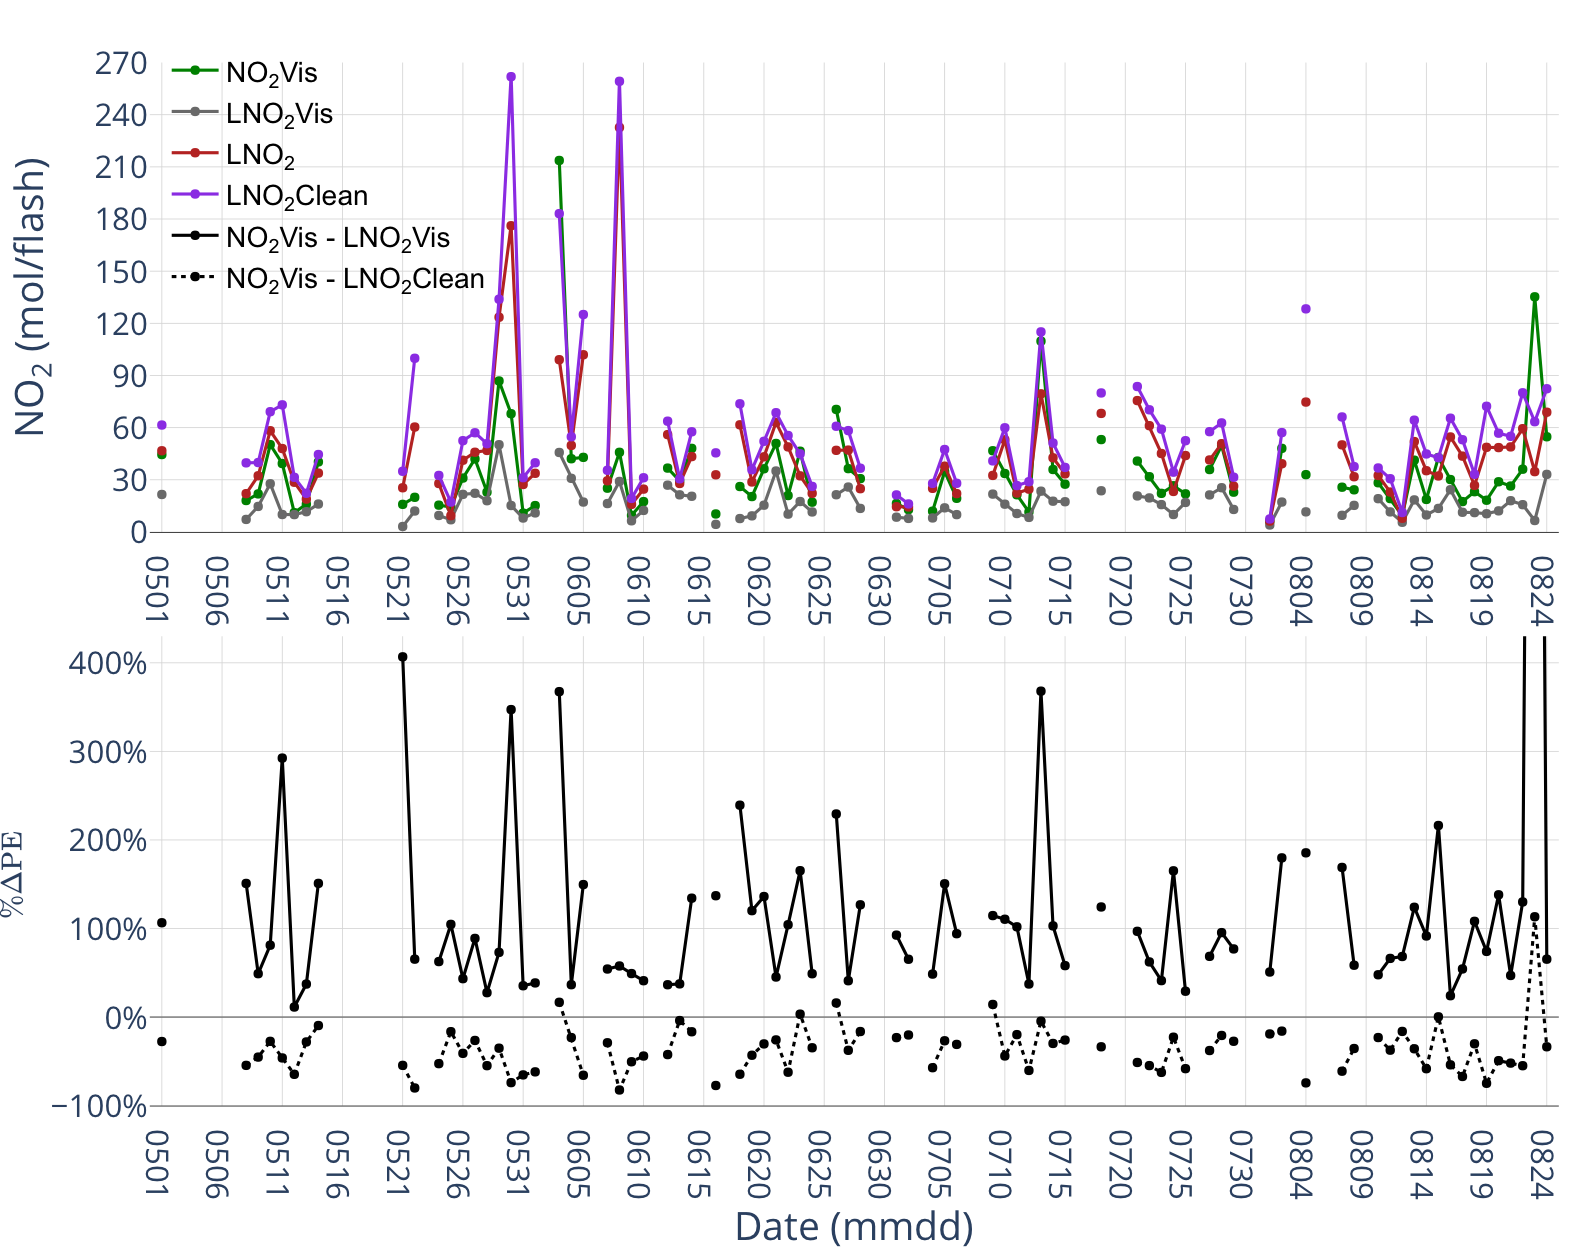
\includegraphics[width=0.9\textwidth]{./figures/us_pe_timeseries.png}
\caption{(上图)2014年5--8月美国大陆的NO$_2$Vis、LNO$_2$Vis、LNO$_2$ 和 LNO$_2$Clean产率的时间序列,筛选条件为CRF $\geq$ 90\% 和每 2.4 小时 至少2400 次闪电;
(下图)在CRF$\geq$ 90\%的条件下,NO$_2$Vis 和 LNO$_2$Vis 之间百分比差异以及 NO$_2$Vis 和 LNO$_2$Clean 之间百分比差异的时间序列。
8 月 23 日黑点的值(未显示)为 1958\%。\\
Figure \ref{fig:us_pe_timeseries}. (top) Time series of NO$_2$Vis, LNO$_2$Vis, LNO$_2$ and LNO$_2$Clean production per day over the CONUS for MJJA 2014 with CRF $\geq$ 90\% and a flash threshold of 2400 flashes per 2.4 h.
(bottom) Time series of the percent differences between NO$_2$Vis and LNO$_2$Vis and the percent differences between NO$_2$Vis and LNO$_2$Clean with CRF $\geq$ 90\%.
The value of black dot on August 23 (not shown) is 1958\%.}
\label{fig:us_pe_timeseries}
\end{figure}


为了将我们的结果与\citet{Lapierre.2020}的结果进行比较,
我们选择了CP $\leq$ 650 hPa、TL $\geq$ 1000 和 ratio $\geq$ 50\% 的条件,
然而我们得到的NO$_2$Vis(3.8 $\pm$ 0.5 mol每闪击)仍大于\citet{Lapierre.2020}的1.6 $\pm$ 0.1 mol每闪击。
这可能是由两者使用不同版本的伯克利高分辨率(BEHR)算法引起的,\citet{Lapierre.2020}使用的是BEHR v3.0A,我们的算法基于BEHR v3.0B \citep{Laughner.2019a}。
两个版本中$S_{\ch{NO2}}$均来自于NASA标准产品v3,BEHR v3.0B 的主要改进如下:

(1)使用最接近 OMI 过境时间的廓线,而不是 OMI 过境之前最后一个时刻的廓线;

(2)使用可变的对流层顶高度,而不是固定的200 hPa 对流层顶;

(3)根据\citet{Zhou.2009}的方法计算地表气压。

% 详细的更新日志见\url{https://github.com/CohenBerkeleyLab/BEHR-core/blob/master/Documentation/Changelog.txt}。
此外,\citet{Lapierre.2020}使用了月平均NO$_2$廓线,而我们的研究使用了日廓线,并且我们将WRF-Chem 输出的间隔调整为 30 min,
这比BEHR 每日产品输出间隔1 h更短,但 AMF 可能还会受到不同 NO$_2$ 廓线的影响。
鉴于这些因素,我们在该研究所得数据的基础上来比较不同的方法,以尽量减少这些影响。

\begin{figure}[H]
\centering
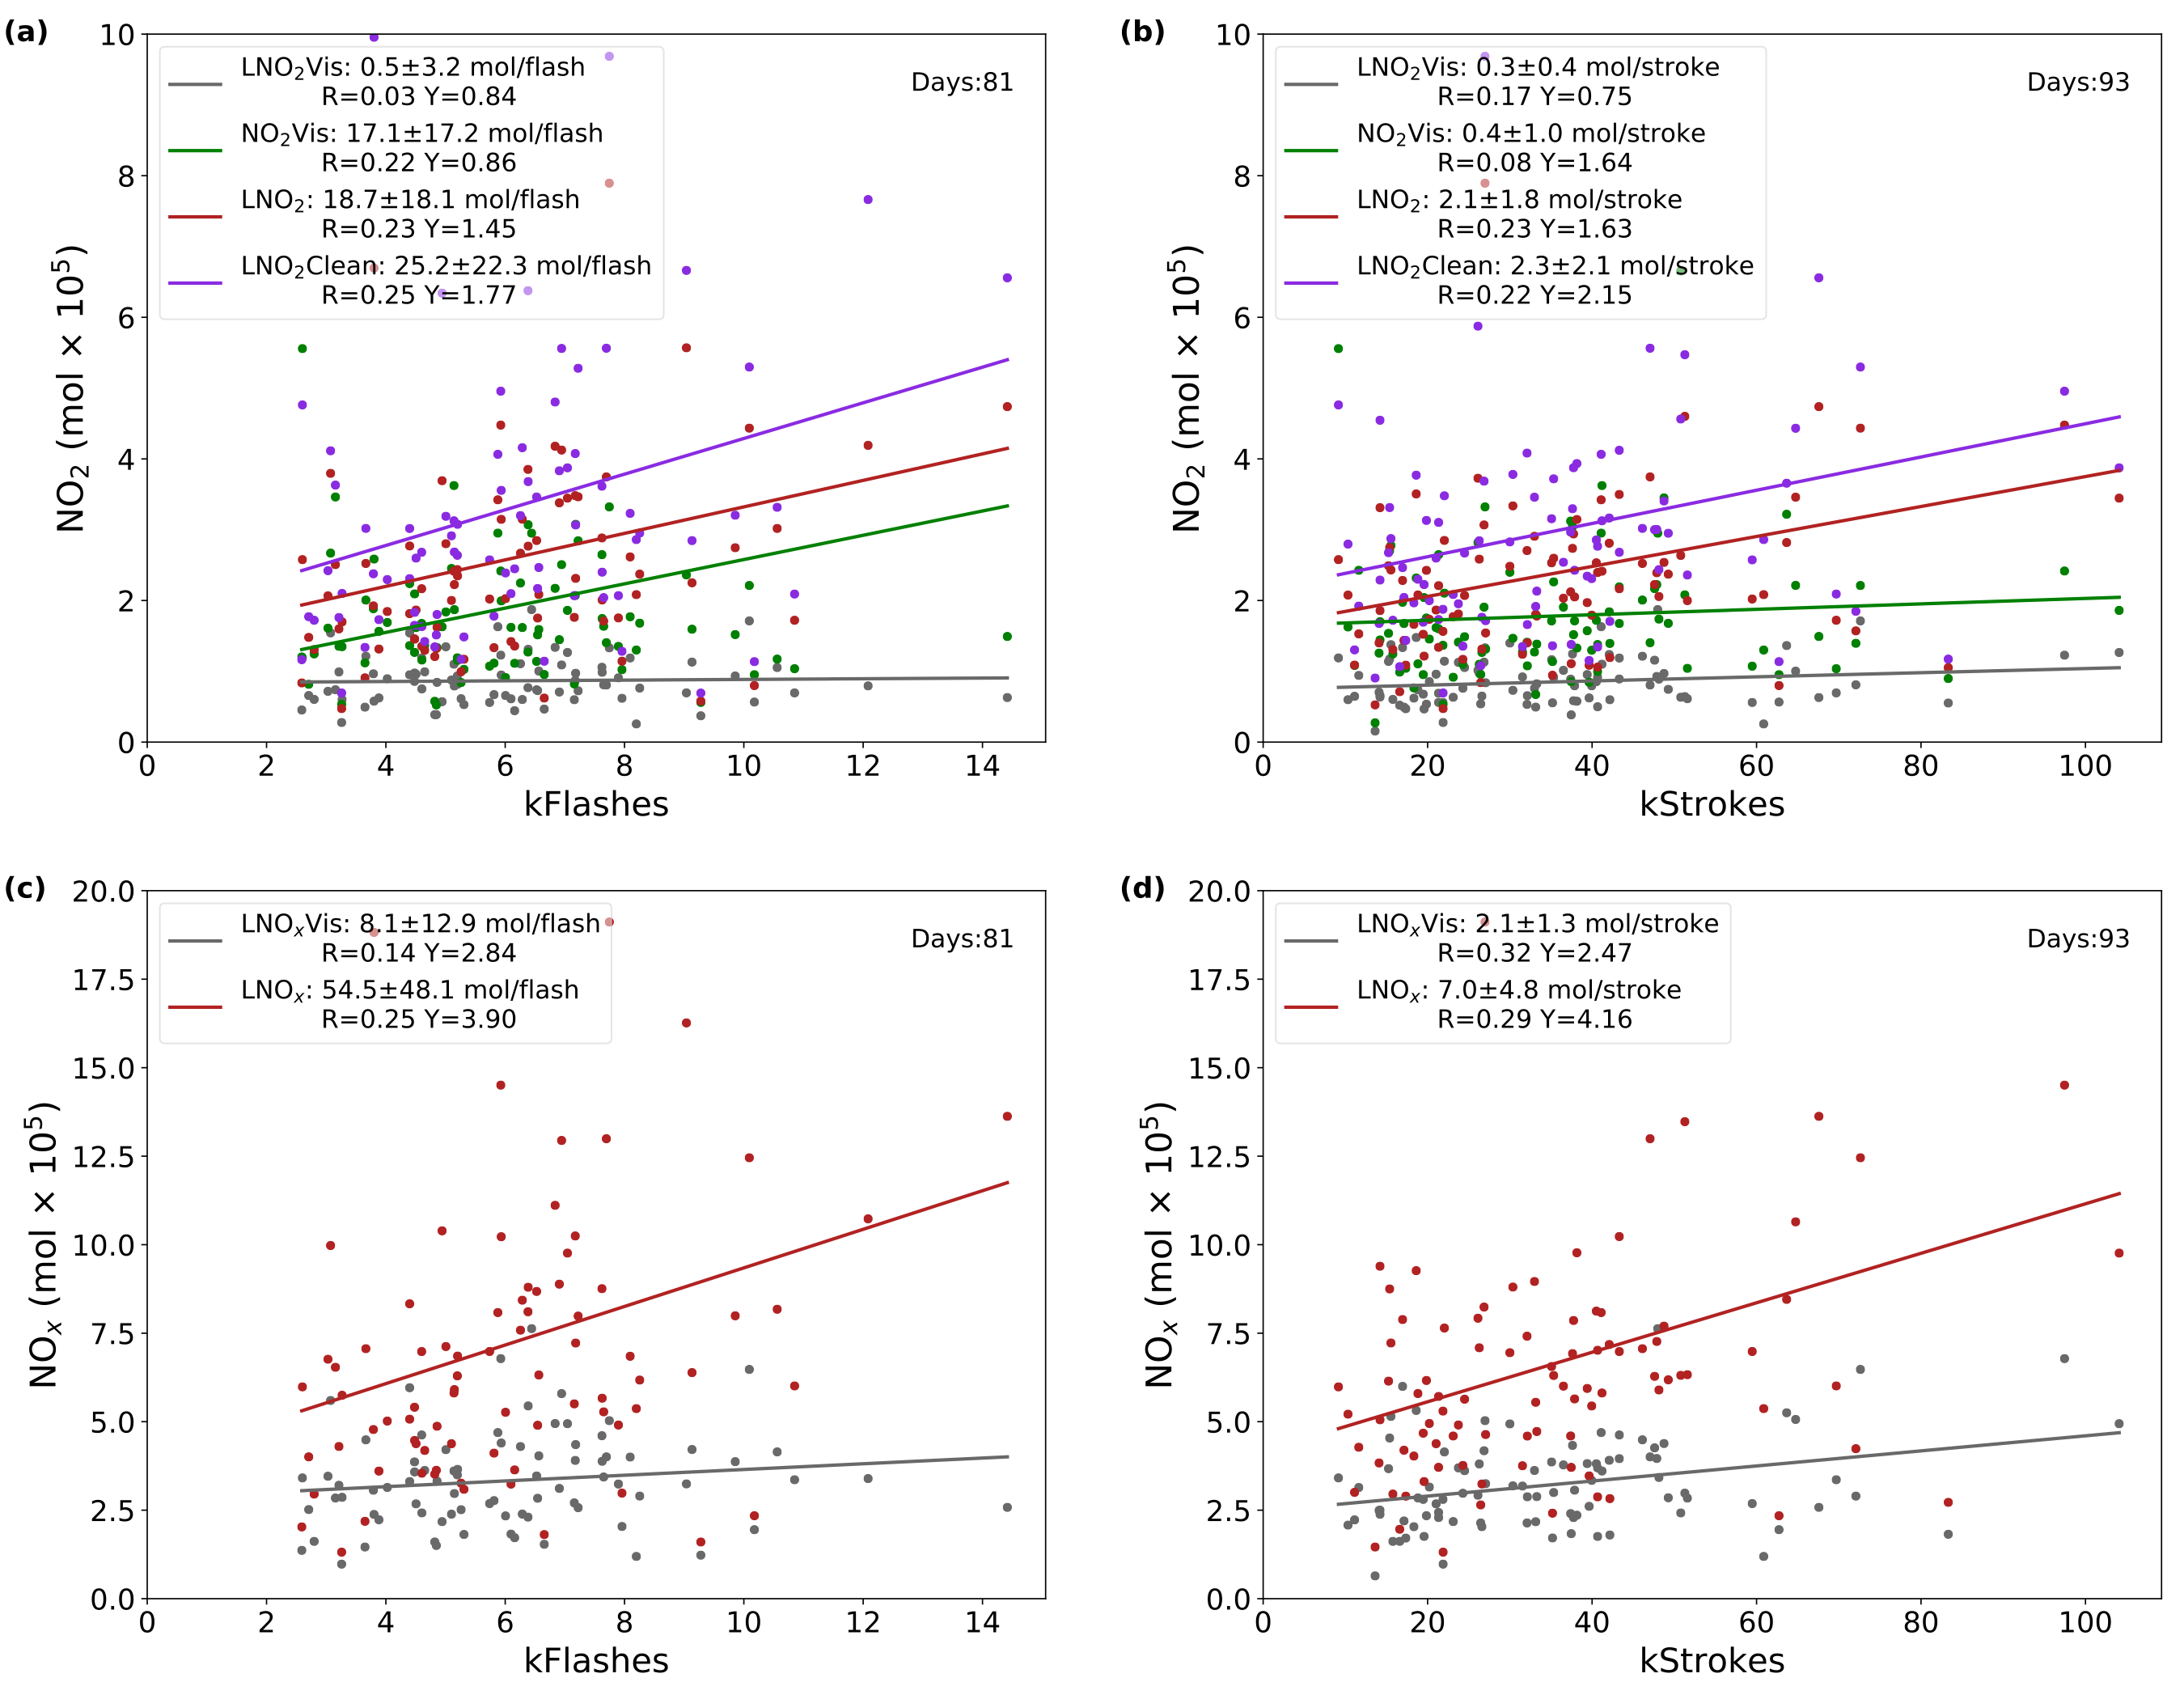
\includegraphics[width=0.95\textwidth]{./figures/us_pe_linear.png}
\caption{(a)每日 NO$_2$Vis、LNO$_2$Vis、LNO$_2$ 和 LNO$_2$Clean 与 ENTLN 总闪的关系;
(b)与(a)相同,但针对闪击数据;
(c)每日LNO$_x$Vis 和 LNO$_x$ 与总闪的关系;
(d)与(c)相同,但针对闪击数据。\\
Figure \ref{fig:us_pe_linear}.
(a) Daily NO$_2$Vis, LNO$_2$Vis, LNO$_2$ and LNO$_2$Clean versus ENTLN total flashes data.
(b) Same as (a) but for strokes.
(c) Daily LNO$_x$Vis and LNO$_x$ versus total flashes.
(d) Same as (c) but for strokes.}
\label{fig:us_pe_linear}
\end{figure}

\begin{figure}[H]
\centering
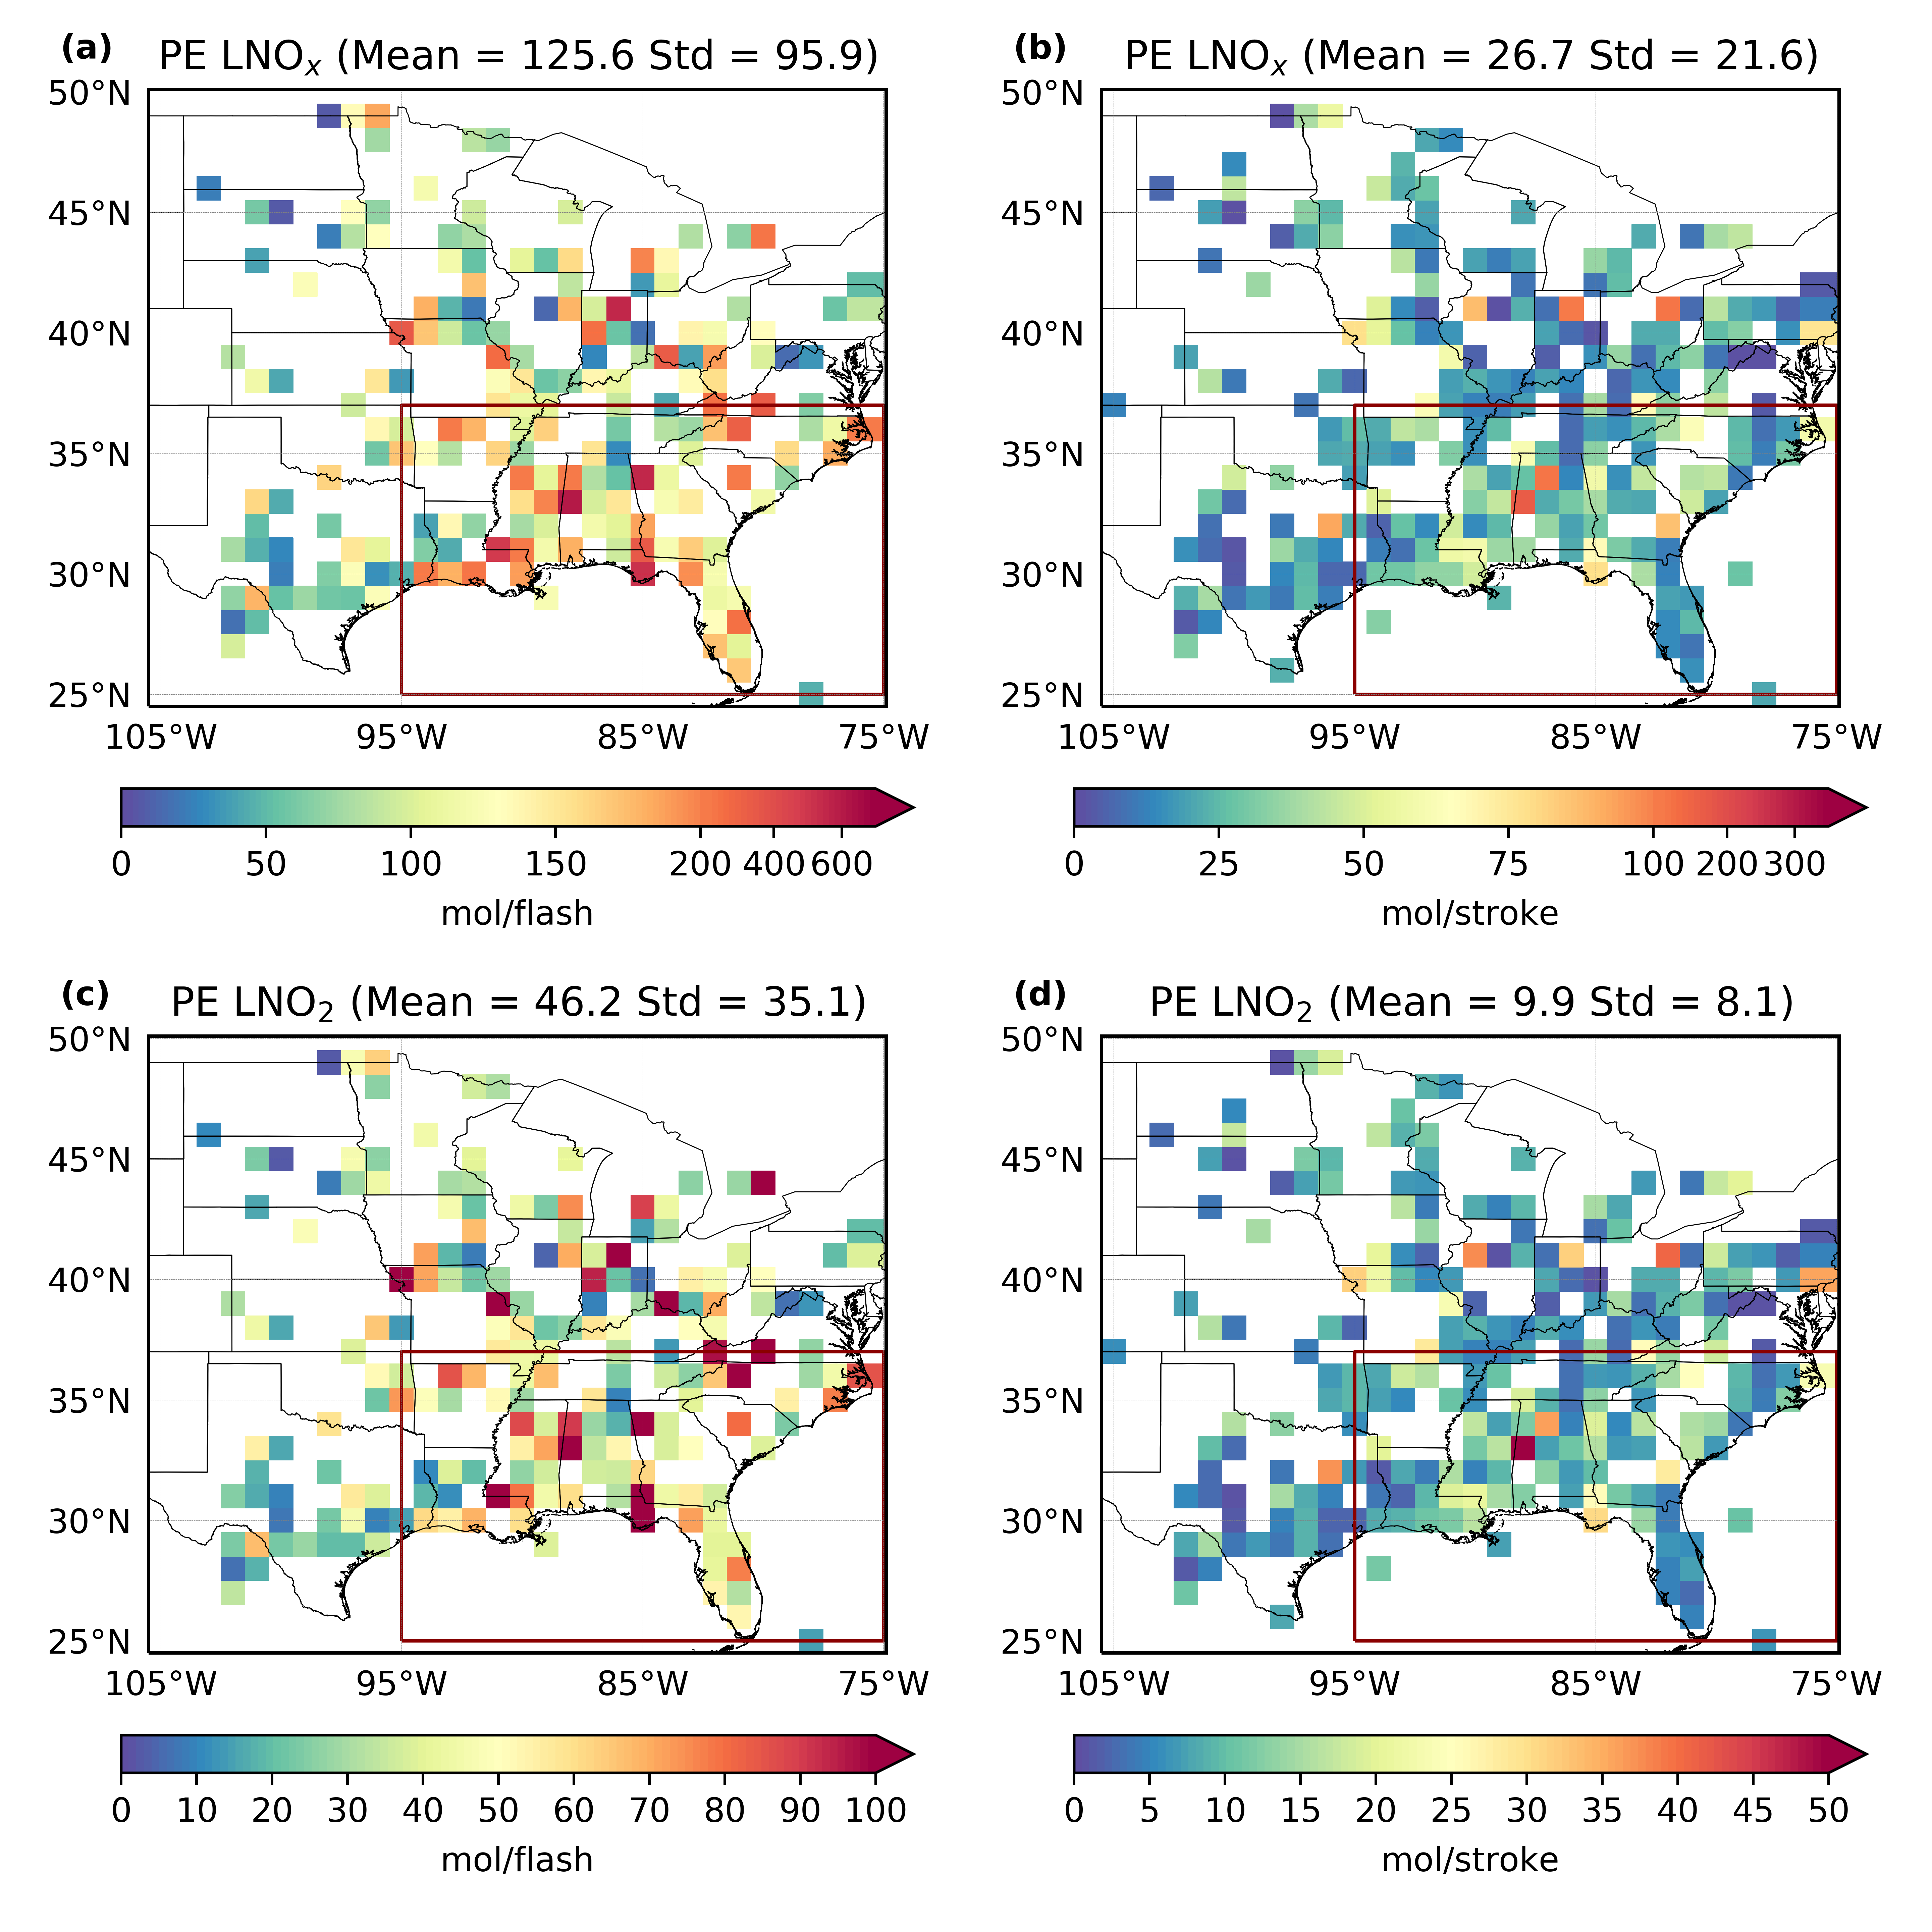
\includegraphics[width=0.95\textwidth]{./figures/us_pe_sum.png}
\caption{(a,c)在CRF $\geq$ 90\%条件下,2014年5--8月 1$^{\circ}$ $\times$ 1$^{\circ}$ LNO$_x$ 和LNO$_2$的平均产率分布图;
     (b,d) 与 (a,c) 相同,但针对闪击数据。
     a--d中的红框表示美国东南部。\\
     Figure \ref{fig:us_pe_sum}. (a) and (c) Maps of 1$^{\circ}$ $\times$ 1$^{\circ}$ gridded values of mean LNO$_x$
    and LNO$_2$ production per flash with CRF $\geq$ 90\% for MJJA 2014.
    (b) and (d) Same as (a) and (c) except for strokes.
    The southeastern US is denoted by the red box in panels a--d.
}
\label{fig:us_pe_sum}
\end{figure}

结果表明,LNO$_2$产率(18.7 $\pm$ 18.1 mol每闪电,2.1 $\pm$ 1.8 mol每闪击)介于 LNO$_2$Clean产率 和 NO$_2$Vis产率之间,
与图 \ref{fig:us_pe_timeseries} 中的日结果一致。
此外,基于每日求和值的线性回归结果得到的LNO$_x$产率为114.8 $\pm$ 18.2 mol每闪电(或17.8 $\pm$ 2.9 mol每闪击),
该结果大于\citet{Pickering.2016}的91 mol每闪电。
这一差异可能是由地理位置、闪电数据和化学模式所共同导致的。
在 CRF $\geq$ 90\% 下,求和法得到LNO$_2$产率为 46.2 $\pm$ 35.1 mol 每闪电和 9.9 $\pm$ 8.1 mol 每闪电,
而 LNO$_x$ 产率为 125.6 $\pm$ 95.9 mol 每闪电和 26.7 $\pm$ 21.6 mol 每闪电(图\ref{fig:us_pe_sum})。
其中美国东南部的 LNO$_2$和 LNO$_x$ 产率均较高(由图\ref{fig:us_pe_sum}中的红框表示,25--37$^{\circ}$ N,75--95$^{\circ}$ W),这与\citet{Lapierre.2020} 和 \citet{Bucsela.2019}的研究结果相一致。
而与图\ref{fig:us_pe_timeseries}相比,图\ref{fig:us_delta}a--b显示
NO$_2$Vis产率和 LNO$_2$Vis产率之间的一些较大差异,这与我们对污染区域的预期一致。
同时,LNO$_2$ 和 NO$_2$Vis产率之间的差异取决于背景 NO$_2$、上升气流的强度和廓线分布。
负差异是由上升气流携带的背景 NO$_2$ 污染引起的,
而云下 LNO$_2$ 的部分导致LNO$_2$产率高于NO$_2$Vis产率(图\ref{fig:us_delta}c)。
图\ref{fig:us_delta}d显示 LNO$_2$Vis在LNO$_2$中占比为 10--80\%,
这可能是由云层的高度和 LNO$_2$ 的廓线造成的。
如果云压在300 hPa附近,由于云层的覆盖,该比值将更小。
因此,LNO$_x$的估算需要更好地了解LNO$_2$和云下LNO$_x$的垂直分布。


\subsection{估算的影响因素及不确定性分析} \label{sec:uncertainty}

图\ref{fig:us_delta}表明,在污染和清洁地区我们方法对于LNO$_2$产率估算的改进程度是不同的。
为了简化量化,我们选择了CRF = 100\%的条件,具有相似云上NO$_2$廓线($\sim$ 100 pptv)的六个网格,这样AMF之间的差异取决于较少的参数:
\begin{equation} \label{AMFLNO2_crf100}
AMF_{\ch{LNO2}} = \frac{\int_{p_{\ch{cloud}}}^{p_{\ch{tp}}} w_{\ch{cloudy}}(p) NO_2(p) \: dp}{\int_{p_{\ch{surf}}}^{p_{\ch{tp}}} LNO_2(p) \: dp}
\end{equation}
\begin{equation} \label{AMFNO2Vis_crf100}
AMF_{\ch{NO2Vis}} = \frac{\int_{p_{\ch{cloud}}}^{p_{\ch{tp}}} w_{\ch{cloudy}}(p) NO_2(p) \: dp}{\int_{p_{\ch{cld}}}^{p_{\ch{tp}}} NO_2(p) \: dp}
\end{equation}
\begin{equation} \label{AMFLNO2Clean_crf100}
AMF_{\ch{LNO2Clean}} = \frac{\int_{p_{\ch{cloud}}}^{p_{\ch{tp}}} w_{\ch{cloudy}}(p) LNO_2(p) \: dp}{\int_{p_{\ch{surf}}}^{p_{\ch{tp}}} LNO_2(p) \: dp}
\end{equation}
这些网格框包含图\ref{fig:us_delta}a中的污染城市(星形)和清洁城市(三角形)。
图\ref{fig:us_bkgd_comp}比较了污染和清洁网格内NO$_2$、背景 NO$_2$ 和背景 NO$_2$占比的平均廓线。
由于对流层上层LNO$_2$ 浓度高于背景 NO$_2$ 浓度,背景 NO$_2$ 与总 NO$_2$ 的比例曲线呈 C 形。
然而,随着背景 NO$_2$ 增加和 LNO$_2$ 的减少,图\ref{fig:us_bkgd_comp}e中的比例在云压和对流层顶之间存在峰值。
此外污染地区的对流层上层背景NO$_2$占比稳定且高于清洁地区。

表\ref{table:production_comp}显示了对于6个城市三种方法之间的相对变化。
AMF$_{\ch{LNO2}}$(式\ref{AMFLNO2_crf100})和 AMF$_{\ch{LNO2Clean}}$(式\ref{AMFLNO2Clean_crf100})之间的区别是分子:
$\int_{p_{\ch{cloud}}}^{p_{\ch{tp}}} w_{\ch{cloudy}}(p) NO_2(p) \: dp$
和$\int_{p_{\ch{cloud}}}^{p_{\ch{tp}}} w_{\ch{cloudy}}(p) LNO_2(p) \: dp$。
当 LNO$_2$ 的比例较高或区域较清洁时,两者相对差异较小(5.0--12.0\%,图\ref{fig:us_bkgd_comp}d--f),
最大的相对差异(46.3\%)发生在对流层上层背景 NO$_2$ 所占比例一直较高的情况下(图\ref{fig:us_bkgd_comp}c)。
因此,我们的方法对背景 NO$_2$ 不太敏感,更适用于受污染地区的对流情况。
相比之下,由于包含了云层下方的 LNO$_2$,我们方法估算的产量大于基于 NO$_2$Vis 的产量。
当云层较高时,特别是 LNO廓线的峰值低于云层时(图\ref{fig:us_bkgd_comp}b),
相对差异较大(121.2\%),因为更多的 LNO$_2$ 不能包含在 NO$_2$Vis 中。
AMF$_{\ch{LNO2Clean}}$(式\ref{AMFLNO2Clean_crf100})和 AMF$_{\ch{NO2Vis}}$(式\ref{AMFNO2Vis_crf100})之间的相对变化取决于
$\int_{p_{\textrm cloud}}^{p_{\textrm tp}} w_{\textrm cloudy}(p) LNO_2(p) \: dp / \int_{p_{\textrm surf}}^{p_{\textrm tp}} w_{\textrm cloudy}(p) LNO_2(p) \: dp$,这也是受云影响,而不是背景NO$_2$。
其中最大的相对变化(153.8\%)发生在新奥尔良,它的云压最小(云层最高),因此可见的柱浓度最小。

图\ref{fig:us_cp_ratio_lno2}a为2014年5--8月在CRF$\geq$90\%的条件下,云压和$V_{\ch{LNO2Vis}}$与$V_{\ch{LNO2}}$之比的日分布。
当云压从600降低到300 hPa时,$V_{\ch{LNO2Vis}}$与$V_{\ch{LNO2}}$之比从 0.8 降低到 0.2,
故在相对清洁的区域,NO$_2$Vis产率小于LNO$_2$产率。
除了 LNO$_2$Vis,LNO$_2$产率也是受云压影响。
对于大于 30 mol每闪击的LNO$_2$产率,云压均小于 550 hPa(图\ref{fig:us_cp_ratio_lno2}b),
而较小的 LNO$_2$ 产率(<30 mol每闪击)出现在 650 hPa 和 200 hPa 之间。
由于较高的LNO$_2$ 产率和闪电数据数量有限,现阶段我们无法推出 LNO$_2$ 产率与云压或其他闪电属性之间的关系。
由于云压仅代表云的发展,因此不能仅从云压值推导出闪电的垂直结构。
前人研究表示,闪电通道的长度会有所不同,并且取决于环境条件\citep{Carey.2016,Mecikalski.2017,Fuchs.2018}。
\citet{Davis.2019}比较了两种闪电:正常闪电和异常闪电。
一般来说,正常闪电是上层带正电和中层带负电,而异常闪电则相反\citep{Williams.1989}。
由于异常闪电中上升气流更强且闪电频率更高,因此异常闪电中的对流层上层LNO$_x$浓度高于正常闪电。



\begin{table}[H]
\caption{基于相同先验廓线但不同估算方法时,产量的百分比变化\\Table \ref{table:production_comp}. The percent changes in the estimated production when using different methods based on the same a priori profiles.}
\scriptsize
\centering
\begin{tabular}{clccc}
\hline
 & 城市$^a$ & (LNO$_2$Clean - LNO$_2$)/LNO$_2$ & (LNO$_2$ - TropVis)/TropVis & (LNO$_2$Clean-TropVis)/TropVis \\
\hline
\multirow{3}{*}{污染地区} & Lansing          & 24.2\%  & 49.5\%   & 85.6\%   \\
                         & New Orleans      & 13.3\%  & 121.2\%  & 153.8\%  \\
                         & Orlando          & 46.3\%  & 37.5\%   & 101.3\%  \\
\hline
\multirow{3}{*}{清洁地区}    & Huron            & 12.0\%  & 56.4\%   & 75.2\%   \\
                            & Charles Town     & 12.0\%  & 82.2\%   & 104.1\%  \\
                            & Tarboro          & 5.0\%   & 86.0\%   & 95.3\%   \\
\hline
\end{tabular}
\begin{tablenotes}
\linespread{1}\footnotesize
\item $^a$城市地址见图\ref{fig:us_delta}a。
\item $^a$Locations are denoted in Fig. \ref{fig:us_delta}a.
\end{tablenotes}
\label{table:production_comp}
\end{table}

\begin{figure}[H]
\centering
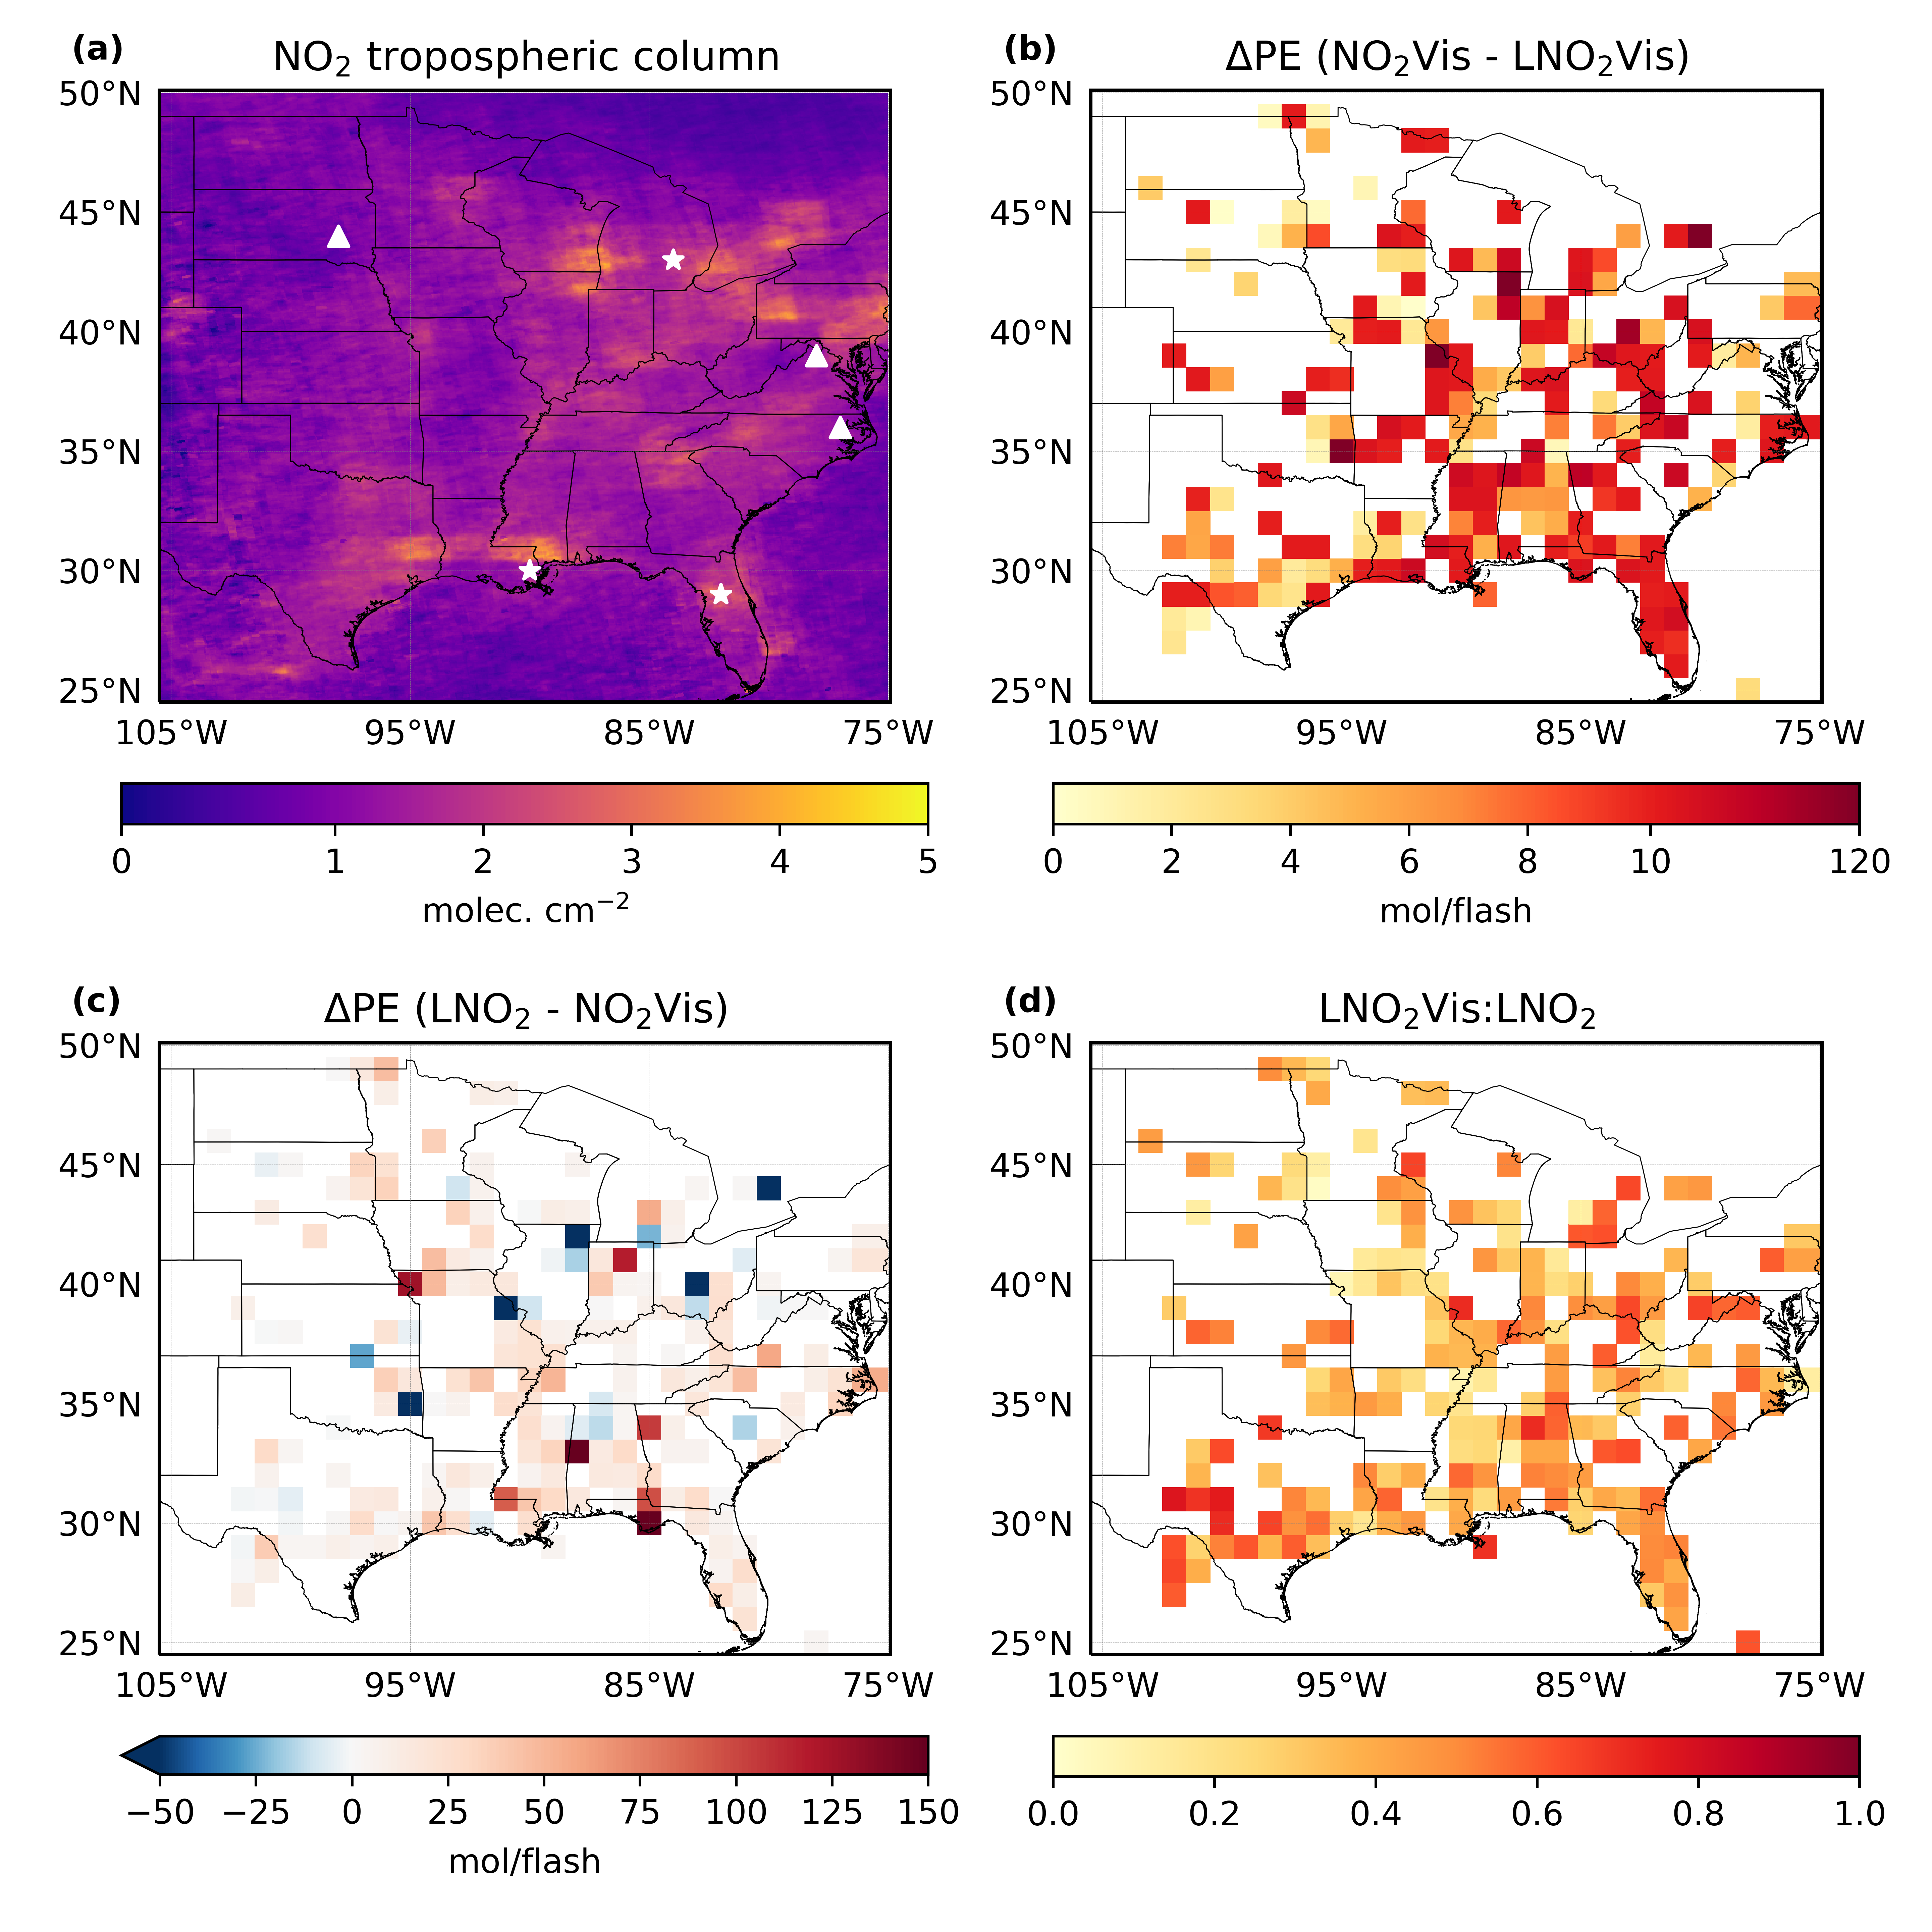
\includegraphics[width=0.95\textwidth]{./figures/us_delta.png}
\caption{(a)2014年5--8月平均对流层NO$_2$柱浓度,
污染城市用星号表示:兰辛、新奥尔良和奥兰多,而清洁城市用三角形表示:休伦、查尔斯镇和塔伯勒;
(b)在CRF $\geq$ 90\%条件下,NO$_2$Vis 和 LNO$_2$Vis平均产率的差异;
(c)与(b)相同,但为 LNO$_2$ 和 NO$_2$Vis 之间的差异;
(d)LNO$_2$Vis 与 LNO$_2$ 的比例。\\
Figure \ref{fig:us_delta}.
(a) Mean NO$_2$ tropospheric column for MJJA 2014.
Polluted cities are denoted by stars: Lansing, New Orleans and Orlando, while clean cities are denoted by triangles: Huron, Charles Town and Tarboro.
(b) The differences of the estimated mean production efficiency between NO$_2$Vis and LNO$_2$Vis with CRF $\geq$ 90\%.
(c) The same differences as (b) but between LNO$_2$ and NO$_2$Vis.
(d) The ratio of LNO$_2$Vis to LNO$_2$.
}
\label{fig:us_delta}
\end{figure}

% 模式中LNO$_x$的分布主要有两种方法:已通过对流输送重新分布的LNO$_x$廓线(对流后)和在对流输送重新分布之前LNO$_x$的廓线(对流前)\citep{Allen.2012,Luo.2017}。
% 然而,鉴于与其他 LNO$_x$ 研究相比结果的相似性,我们相信本文研究中基于对流后LNO$_x$廓线的1$^{\circ}$ $\times$ 1$^{\circ}$结果足以估计LNO$_x$的平均产量。
WRF-Chem中LNO排放的设置在不同的研究中有所不同。
\citet{Zhao.2009}在区域尺度模式中将NO$_x$产率设定为250 mol NO每闪电,
而 \citet{Bela.2016}选择了\citet{Barth.2012}使用的330 mol NO每闪电。
\citet{Wang.2015a}假设每次闪电产生大约 500 mol NO,这是通过云尺度化学传输模式和云中飞机观测得出的\citep{Ott.2010}。
为了评估 LNO$_x$参数化对 LNO$_x$估算的影响,
我们将基于另一个LNO设置(2$\times$基本闪率,500 mol NO每闪电,以下简称“2$\times$500 mol NO每闪电”)的WRF-Chem NO$_2$模拟廓线
应用于先验廓线,并评估 AMF$_{\ch{LNO$_2$}}$、AMF$_{\ch{LNO$_x$}}$、LNO$_2$产率和 LNO$_x$产率相对于1$\times$200 mol NO 每闪电所得结果的变化。
对于线性回归方法(图 \ref{fig:us_pe_linear_2x500}),LNO$_2$产率为 29.8 $\pm$ 20.5 mol每闪电,
比基本设置所得结果(18.7 $\pm$ 18.1 mol每闪电)大59.4\%,
与此同时LNO$_x$产率(从54.5 $\pm$ 48.1 mol每闪电增加到88.5 $\pm$ 61.1 mol每闪电)也取决于 WRF-Chem 中 LNO产率的设置。
通过比较图\ref{fig:us_pe_linear}和图\ref{fig:us_pe_linear_2x500},我们发现当LNO$_2$和NO$_2$Vis产率呈现相同趋势时,
LNO$_2$Clean和 LNO$_2$产率更相似。
目前尚不清楚 NO--NO$_2$--O$_3$ 循环或其他 LNO$_x$ 汇对LNO$_x$产率变化的贡献,
这需利用 WRF-Chem进行详细的来源解析,超出了目前本研究的范围。

\begin{figure}[H]
\centering
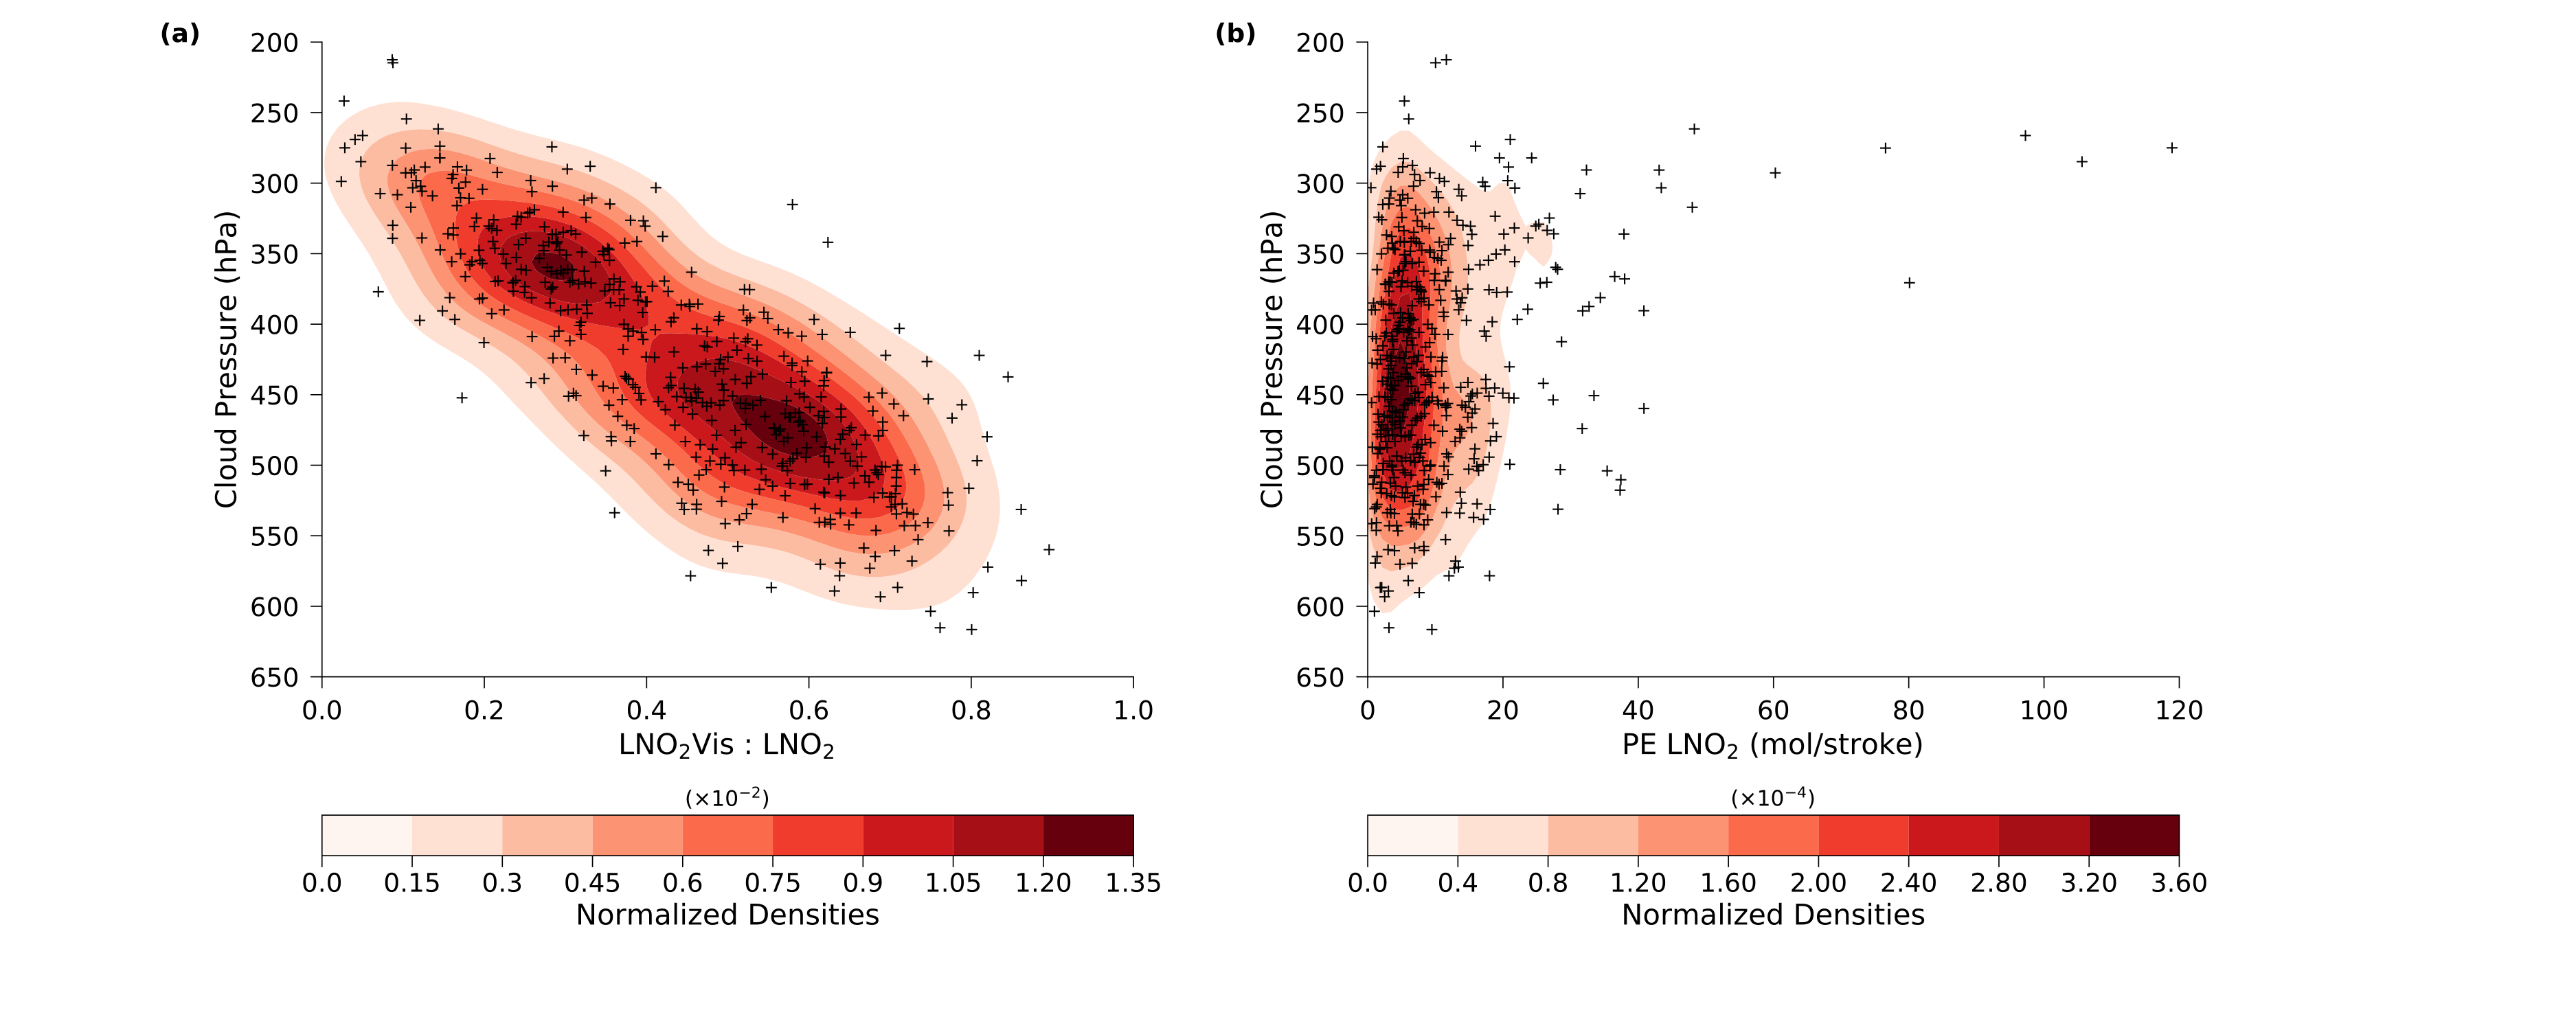
\includegraphics[width=0.9\textwidth]{./figures/us_cp_ratio_lno2.png}
\caption{(a)$V_{\ch{LNO2Vis}}$与$V_{\ch{LNO2}}$之比的核密度估计;(b)LNO$_2$产率与OMI测得云压的核密度估计(2014年5--8月,CRF $\geq$ 90\%)。\\
Figure \ref{fig:us_cp_ratio_lno2}. Kernel density estimation of the (a) daily ratio of $V_{\ch{LNO2Vis}}$ to $V_{\ch{LNO2}}$ and (b) daily LNO$_2$ production efficiency (PE) versus the daily cloud pressure measured by OMI with CRF $\geq$ 90\% for MJJA 2014.}
\label{fig:us_cp_ratio_lno2}
\end{figure}

图\ref{fig:us_simulation_diff}显示了基于 1$\times$200 和 2$\times$500 mol NO 每闪电得到的AMF$_\textrm{LNO$_2$}$、AMF$_\textrm{LNO$_x$}$、LNO$_2$和 LNO$_x$ 的平均百分比变化。
更高的LNO产率设置对LNO$_2$和 LNO$_x$的影响趋势相同:较小的AMF$_\textrm{LNO$_2$}$和AMF$_\textrm{LNO$_x$}$导致较大的LNO$_2$和 LNO$_x$,但变化幅度具有区域性。
这是由AMF$_\textrm{LNO$_2$}$和AMF$_\textrm{LNO$_x$}$的非线性计算引起的。
随着LNO$_2$的贡献增大,AMF方程式的分子和分母都增大。
因为LNO$_2$只占云上NO$_2$的一小部分,分母增加的幅度可能与分子增加的幅度不同,从而对AMF$_\textrm{LNO$_2$}$和AMF$_\textrm{LNO$_x$}$产生不同的影响。
如\citet{Zhu.2019}所述,使用 2$\times$500 mol NO 每闪电的设置和与我们相同的闪电参数化可能会高估美国东南部的闪电密度。
幸运的是,该地区的 AMF 和估算得到的LNO$_2$变化不大。
由于美国东南部的闪电密度最高,因此 AMF 分子中的NO$_2$以LNO$_2$为主,
当模式使用较高的LNO$_2$时,分子和分母增幅相当。
换言之,对 LNO 设置的敏感性降低,LNO$_2$的相对分布很重要。

\begin{figure}[H]
\centering
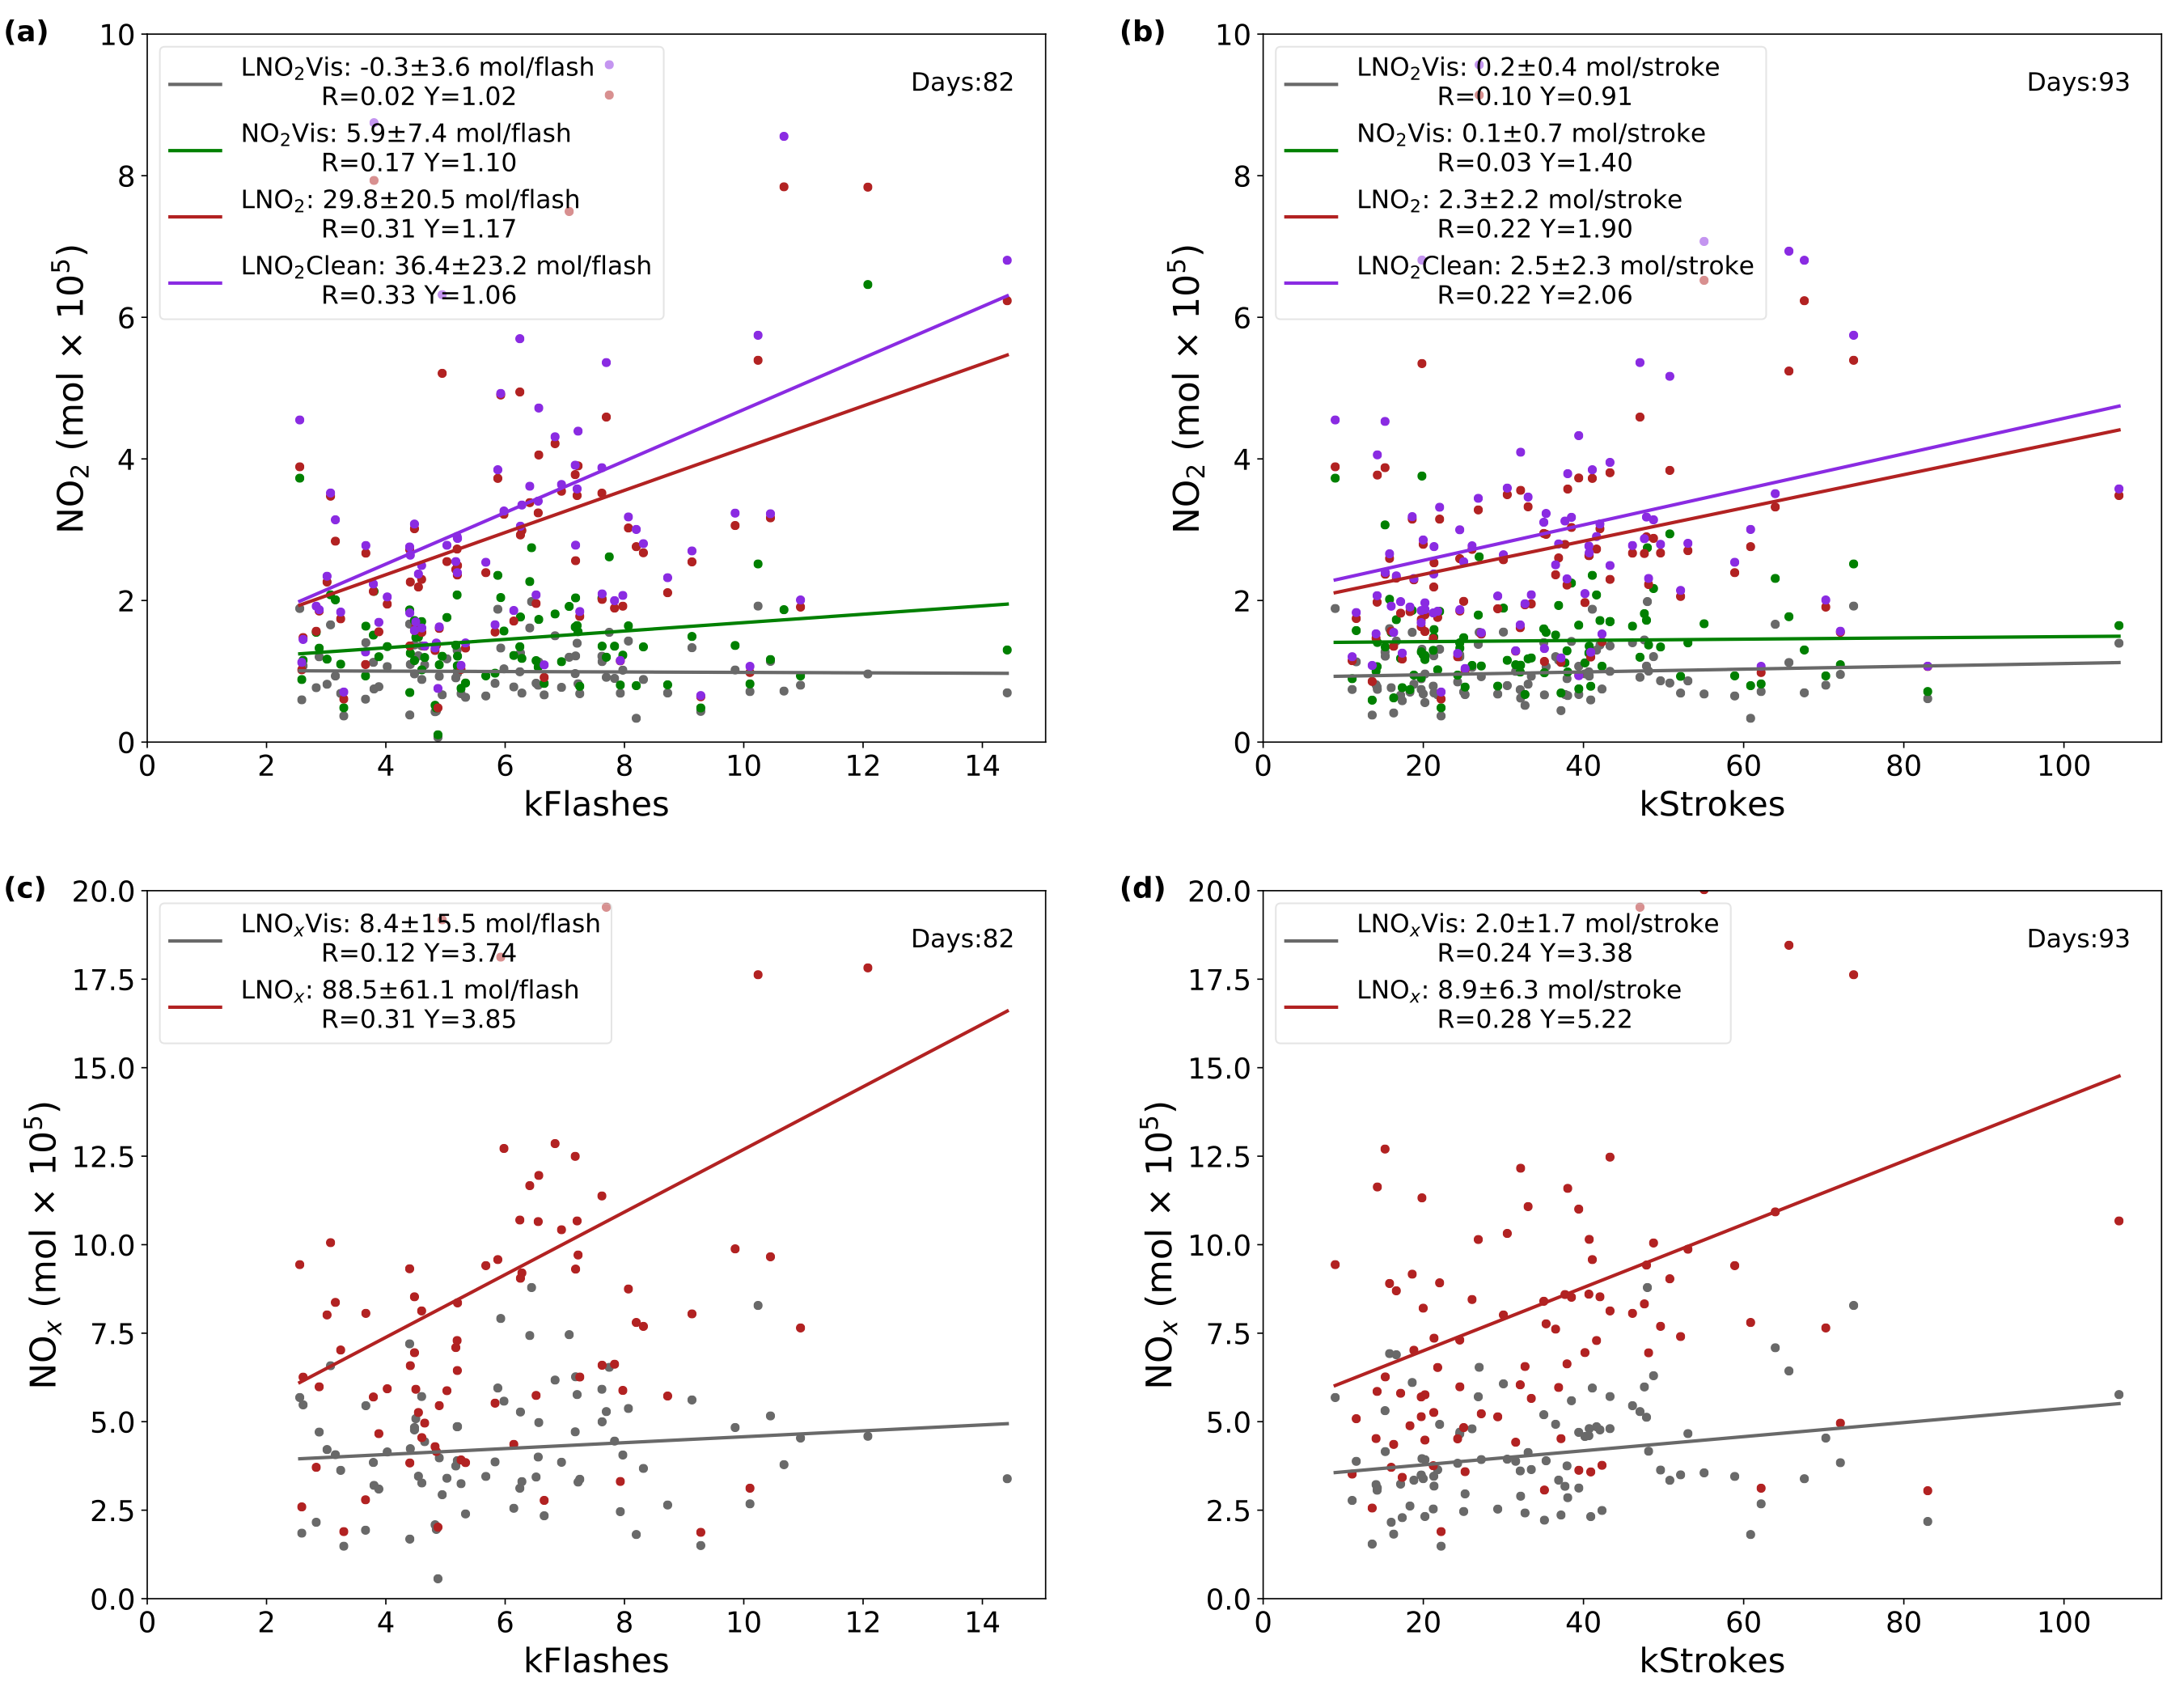
\includegraphics[width=0.95\textwidth]{./figures/us_pe_linear_2x500.png}
\caption{与图\ref{fig:us_pe_linear}相同,但是模式中NO产率设置为2$\times$500 mol每闪电 \\Figure \ref{fig:us_pe_linear_2x500}. Same as Fig. \ref{fig:us_pe_linear} except for the 2$\times$500 mol NO flash$^{-1}$ configuration.}
\label{fig:us_pe_linear_2x500}
\end{figure}


\begin{sidewaysfigure}[htbp!]
\centering
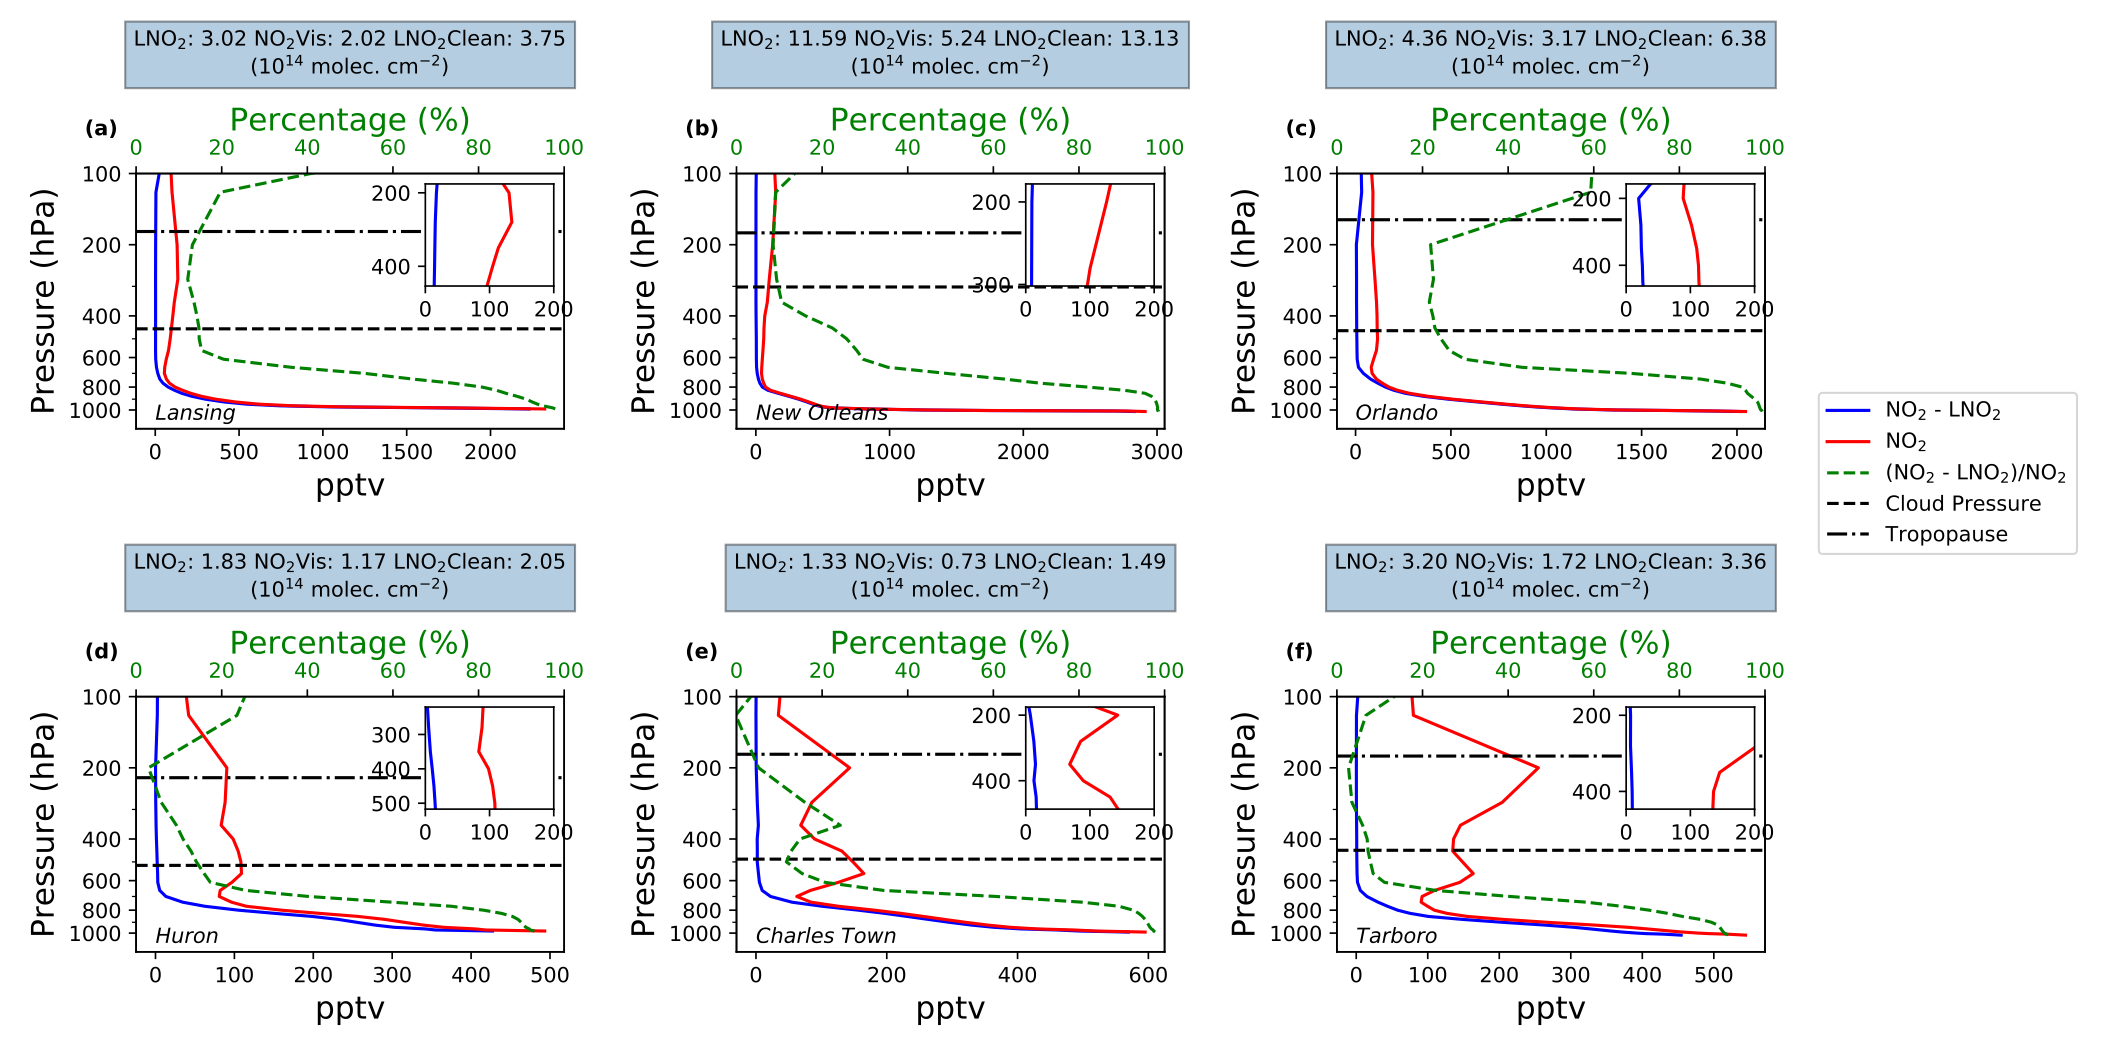
\includegraphics[width=0.9\columnwidth]{./figures/us_bkgd_comp.png}%
\caption{在CRF $\geq$ 100\%条件下,六个网格中WRF-Chem 平均NO$_\textrm{2}$ 和背景 NO$_\textrm{2}$ 廓线。
顶行数据选自污染区域(图 \ref{fig:us_delta}a中的星号),而底行数据来自清洁区域(图 \ref{fig:us_delta}a中的三角形)。
绿色虚线是背景 NO$_\textrm{2}$ 与总 NO$_\textrm{2}$ 的平均比例廓线。
放大图显示了从云压到对流层顶的廓线。
标题基于\ref{sec:amf_definition}节定义的三种不同方法估算得到的产量。\\
Figure \ref{fig:us_bkgd_comp}. Comparisons of mean WRF-Chem NO$_\textrm{2}$ and background NO$_\textrm{2}$ profiles in six grids with CRF $\geq$ 100\% on specific days during MJJA 2014.
The top row data are selected from polluted regions (stars in Fig. \ref{fig:us_delta}a) while the bottom row data are from clean regions (triangles in Fig. \ref{fig:us_delta}a).
The green dashed lines are the mean ratio profiles of background NO$_\textrm{2}$ to total NO$_\textrm{2}$.
The zoomed figures show the profiles from the cloud pressure to the tropopause.
The titles present the mean productions based on three different methods mentioned in Sect. \ref{sec:amf_definition}.}
\label{fig:us_bkgd_comp}
\end{sidewaysfigure}


图\ref{fig:us_lno2_profile}显示了两个特定区域的平均 LNO 和 LNO$_2$ 曲线的比较,
其中 2$\times$500 mol NO 每闪电设置分别导致两区域较低和较高的 LNO$_2$产率。
第一个所选区域(36--37$^{\circ}$ N,89--90$^{\circ}$ W,图\ref{fig:us_lno2_profile}a)是 LNO$_2$ 负百分比变化最小的区域(图\ref{fig:us_simulation_diff}c),
第二个所选区域(31--32$^{\circ}$ N,97--98$^{\circ}$ W,图\ref{fig:us_lno2_profile}b)是LNO$_2$ 正百分比变化最大的区域(图\ref{fig:us_simulation_diff}c)。
尽管两个区域的平均 LNO 和 LNO$_2$廓线的相对分布相似,但量级相差10 倍。
这意味着 WRF-Chem中闪电参数化的表现具有区域性,并且对流层上层可能会出现不切实际的廓线。
虽然这种敏感性分析在某些地区是错误的,但它可得到由于 LNO 和 LNO$_2$ 廓线而影响NO$_2$的上限。
正如\citet{Laughner.2017}中所讨论的,在多云条件下散射权重是均匀的,并且由于高反照率,NO$_2$ 的灵敏度在不同高度上几乎是恒定的。
但是,我们应仔细考虑对流层上层LNO$_2$ 的相对分布。
如果云层上方的 LNO$_2$ ∕ NO$_2$ 足够大(图\ref{fig:us_lno2_profile}a),
AMF$_{\ch{LNO2}}$ 很大程度上取决于 LNO$_2$Vis 与 LNO$_2$ 的比值,
这与相对分布有关。
当不满足高 LNO$_2$ ∕ NO$_2$ 的条件时,相对分布和比例都很重要(图\ref{fig:us_lno2_profile}b)。


\begin{figure}[H]
\centering
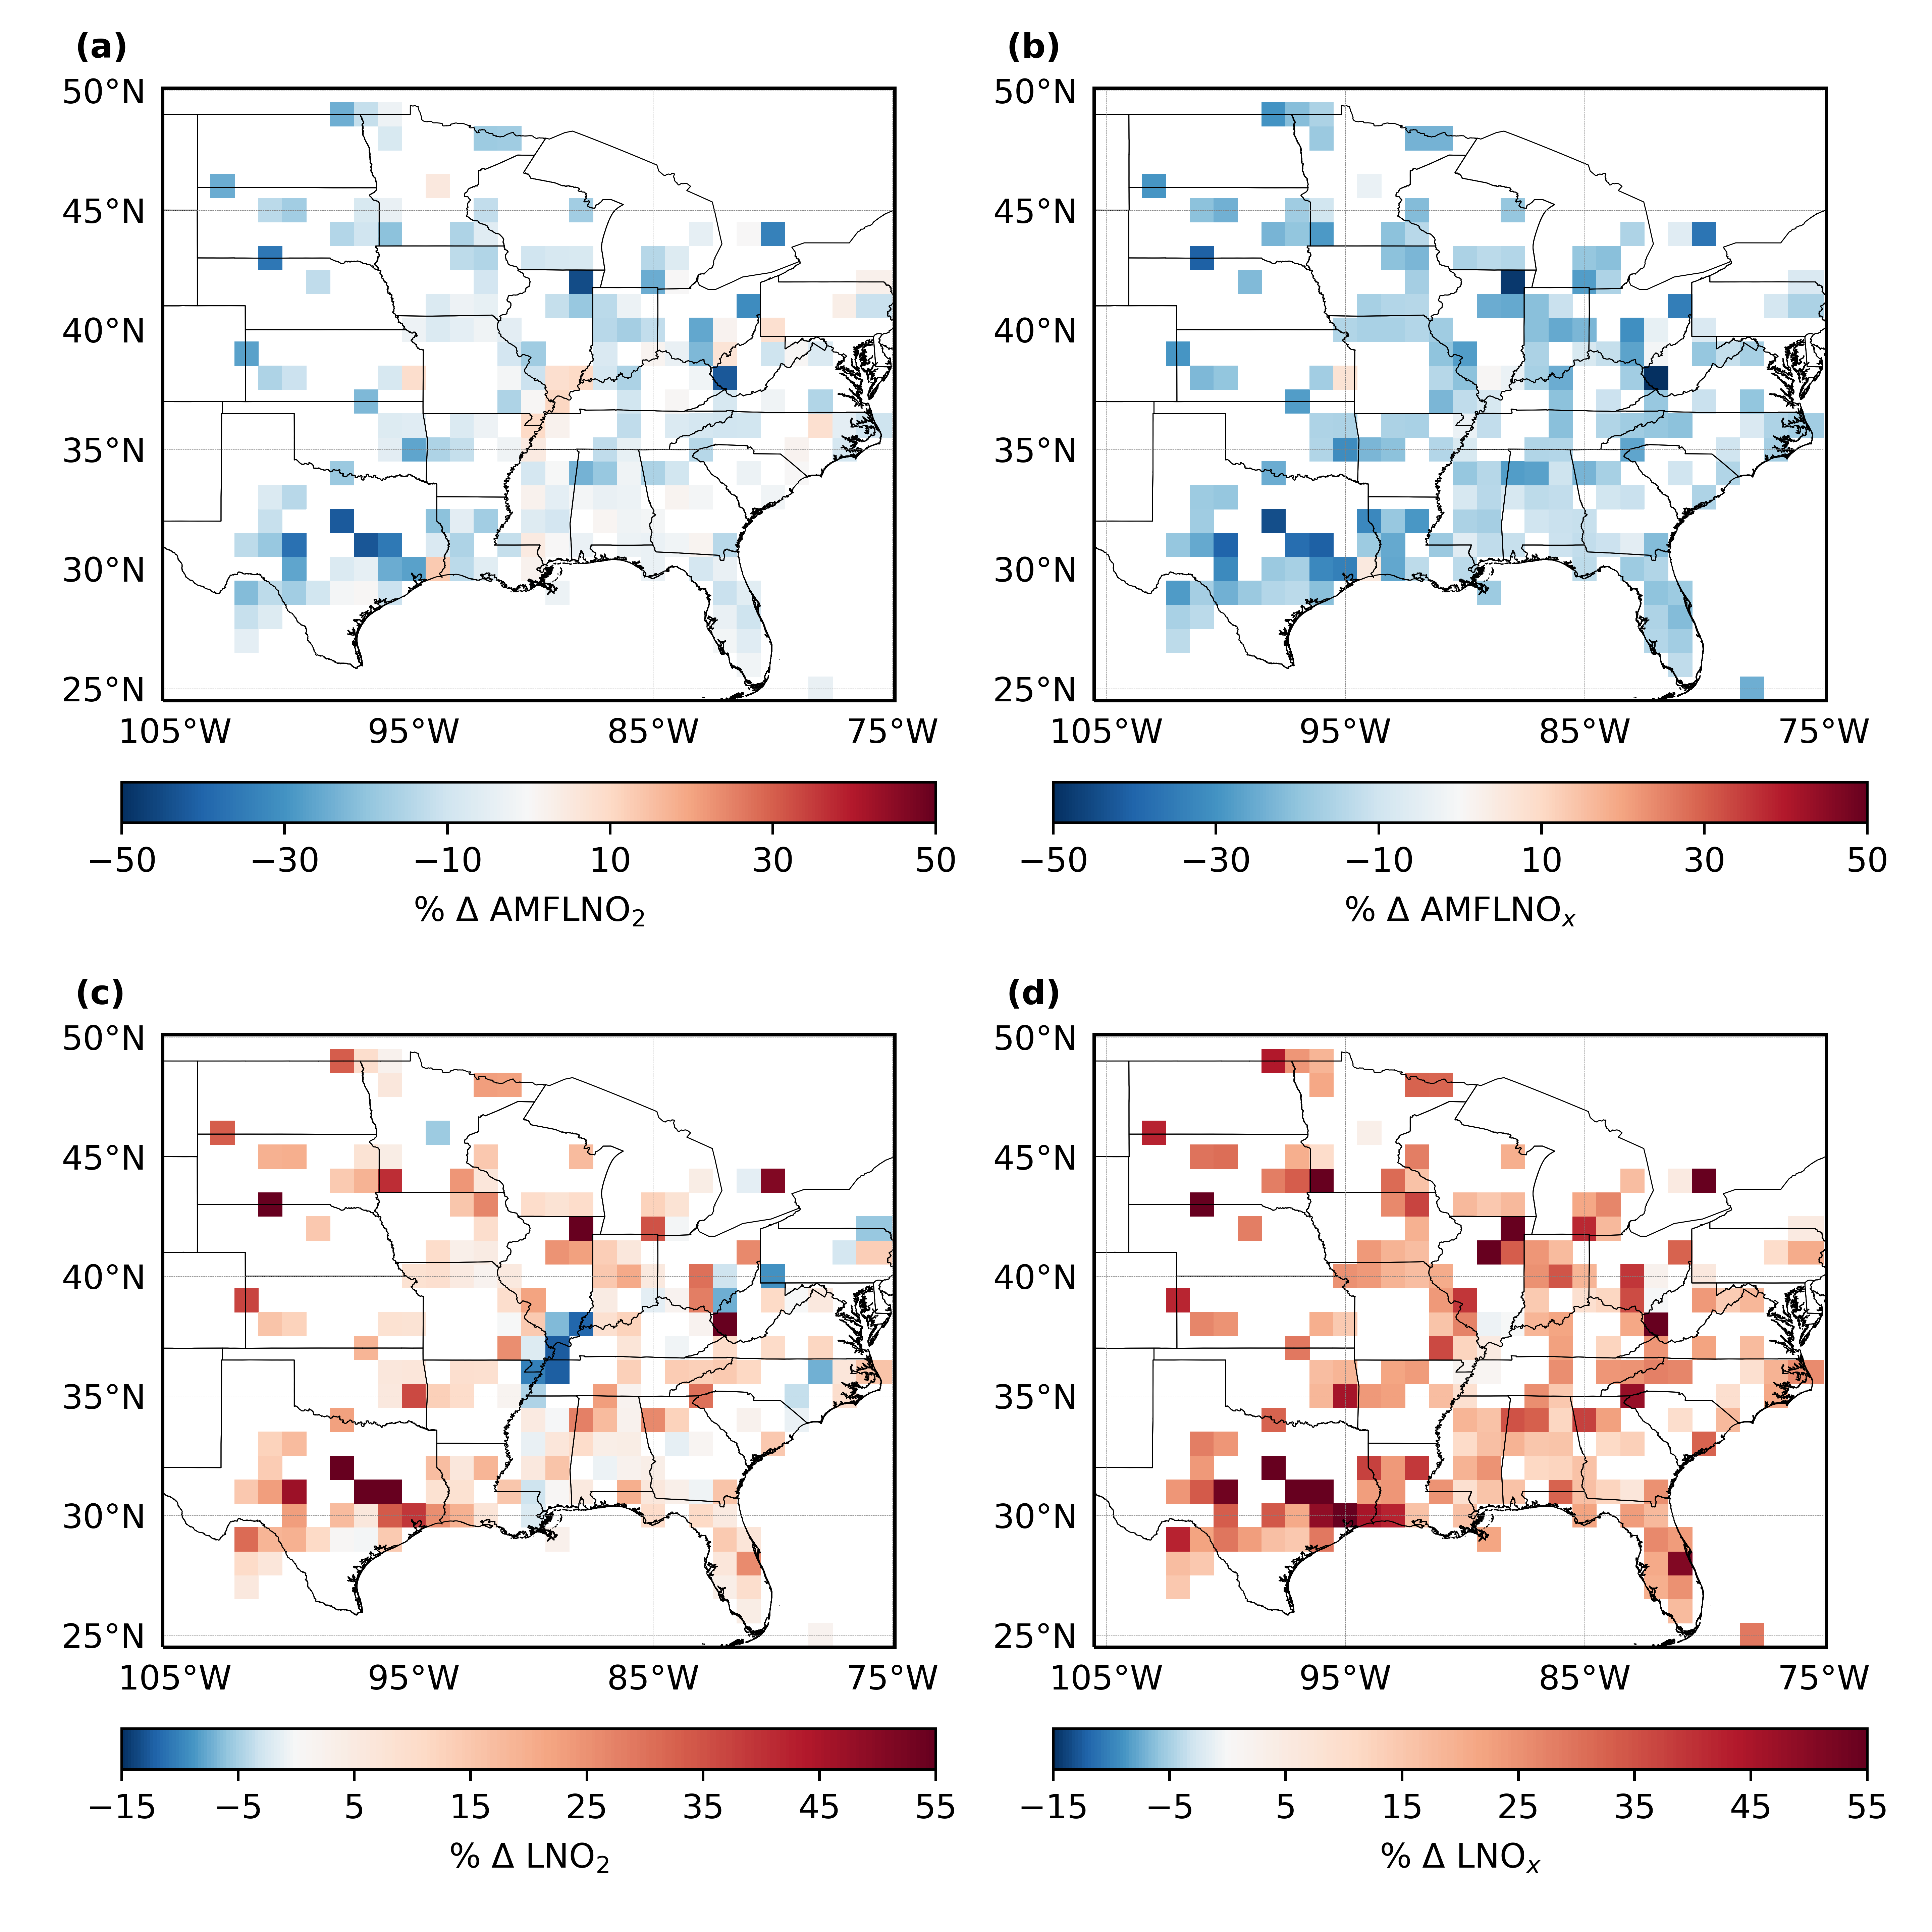
\includegraphics[width=0.9\textwidth]{./figures/us_simulation_diff.png}
\caption{2014年5--8月在CRF $\geq$ 90\% 条件下,
(a)AMF$_{\textrm{LNO$_2$}}$;(b)AMF$_{\textrm{LNO$_x$}}$;
(c)LNO$_\textrm{2}$ 和 (d) LNO$_\textrm{x}$的平均百分比差异。
该差异为 2$\times$500 mol NO每闪电 和 1$\times$200 mol NO每闪电所得结果之差。\\
Figure \ref{fig:us_simulation_diff}. Average percent differences in (a) AMF$_{\textrm{LNO$_2$}}$, (b) AMF$_{\textrm{LNO$_x$}}$, (c) LNO$_\textrm{2}$ and (d) LNO$_\textrm{x}$ with CRF $\geq$ 90\% over MJJA 2014.
Differences are generated by 2$\times$500 mol NO flash$^{-1}$ and 1$\times$200 mol NO flash$^{-1}$.}
\label{fig:us_simulation_diff}
\end{figure}

为了说明这一点,我们使用了不同的LNO产率设置来对LNO$_2$、LNO$_2$Vis、LNO$_2$Clean 和 NO$_2$Vis进行敏感性试验(图\ref{fig:us_lno2_profile})。
其中CRF 的阈值设置为 100\% 以简化等式。
总体上来说,LNO$_2$Clean 和 NO$_2$Vis 的差异小于 LNO$_2$ 和 LNO$_2$Vis 的差异。
通过比较方程中的分子和分母,可得知为何不同的LNO排放设置产生的影响在图\ref{fig:us_lno2_profile}c和d中较小。
对于 LNO$_2$Clean 和 NO$_2$Vis,当更多(更少)LNO$_2$ 或 NO$_2$ 存在时,S$_{\ch{NO2}}$ 和 V$_{\ch{NO2}}$ 都会增加(减少)。
图\ref{fig:us_lno2_profile}a和b的区别是分母,分别为总对流层 LNO$_2$ 垂直柱浓度和可见 LNO$_2$ 垂直柱浓度,
因此图\ref{fig:us_lno2_profile}a中的负值是由云下的 LNO$_2$ 部分引起的。
该误差可导致LNO$_2$ 和 LNO$_x$产率的不确定性,我们保守估计分别为 $\pm$13\% 和 $\pm$25\%。
最终LNO$_2$ 和 LNO$_x$产率的不确定性是根据\citet{Pickering.2016,Allen.2019,Bucsela.2019,Lapierre.2020}的方法得到,即通过依次扰动每个参数来重新计算LNO$_2$ 和 LNO$_x$,从而得到不确定性(表\ref{table:us_uncertainty})。


\begin{figure}[H]
\centering
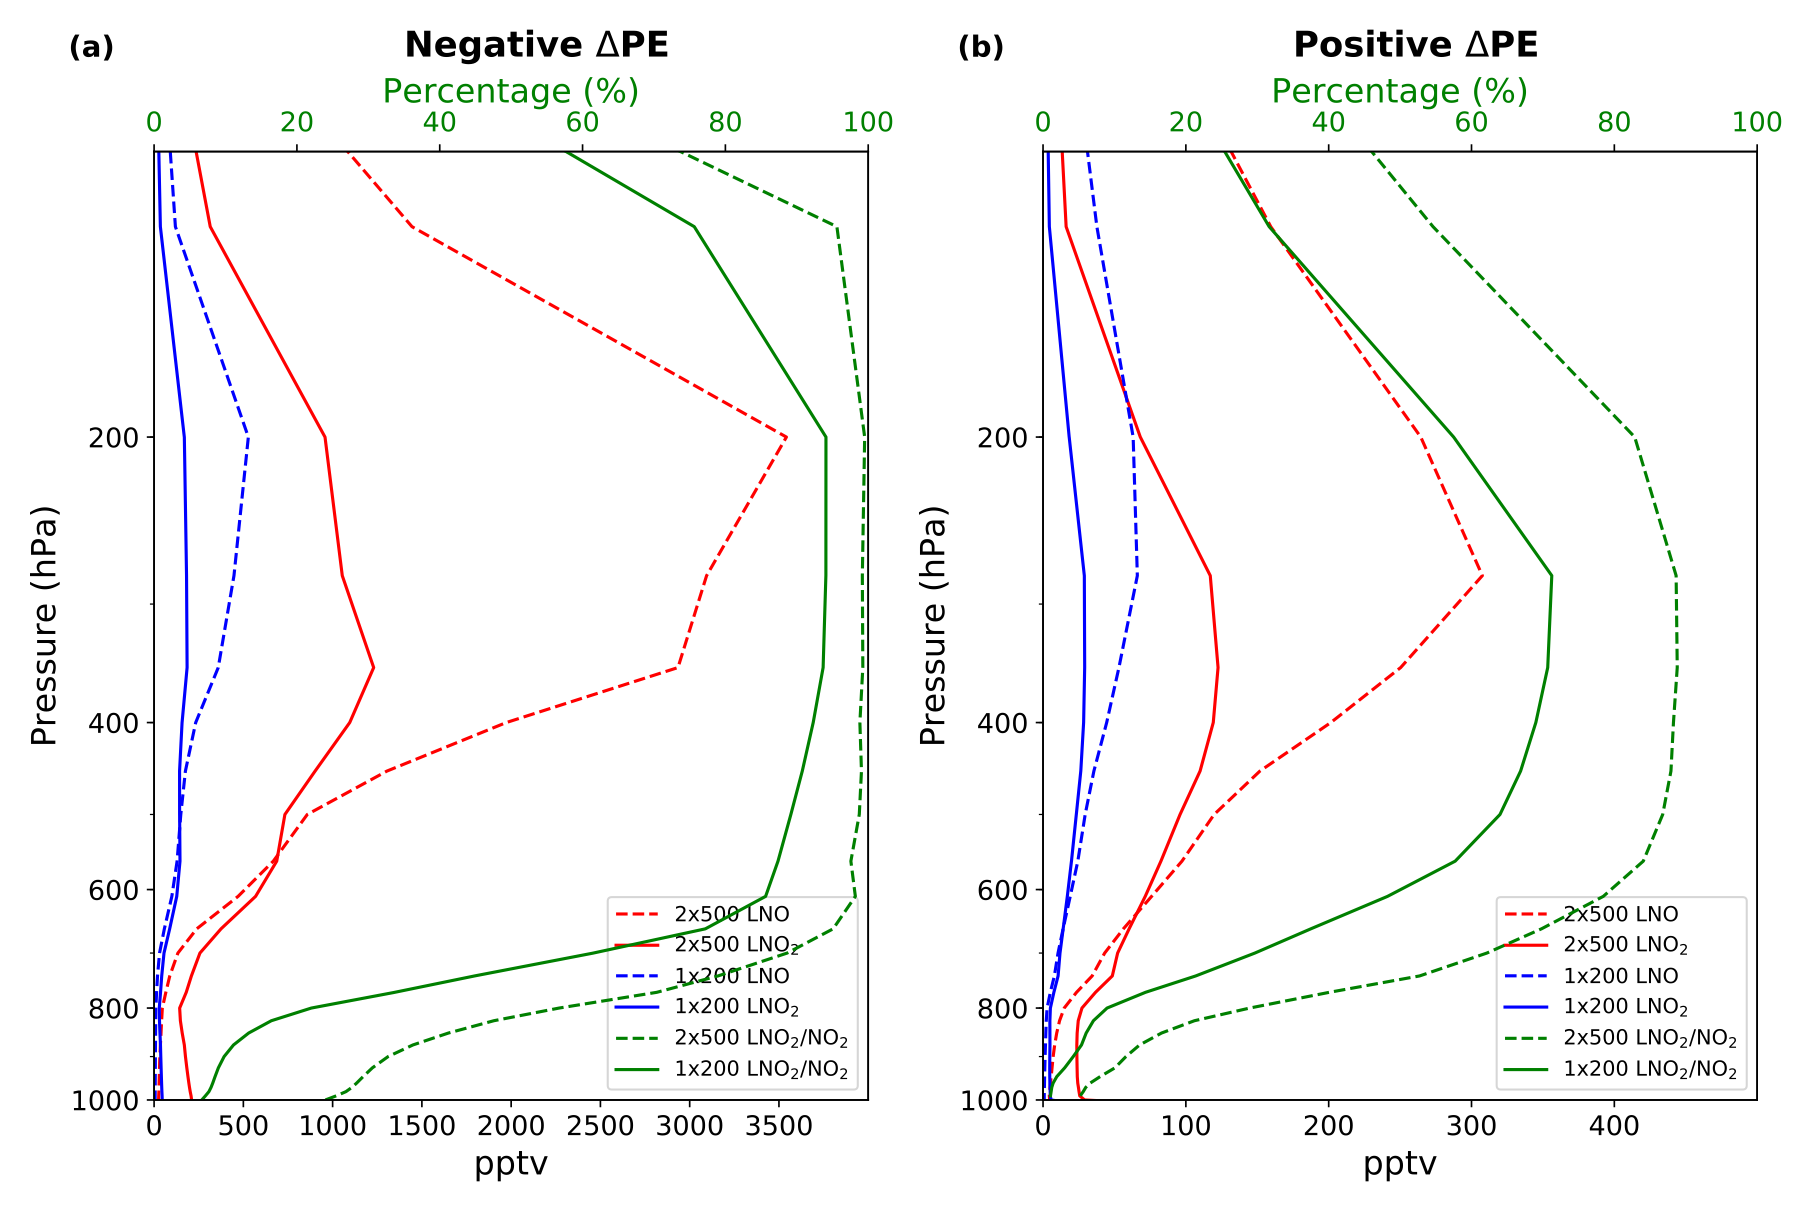
\includegraphics[width=0.9\textwidth]{./figures/us_lno2_profile.png}
\caption{当LNO 设置从 1$\times$200 mol NO每闪电 更改为 2$\times$500 mol NO每闪电 时,
(a)包含 LNO$_2$ 的最小负百分比变化的区域和(b)包含最大正百分比变化的区域中LNO 和 LNO$_2$ 的平均廓线廓线。
使用 1$\times$200(2$\times$500)mol NO每闪电的曲线以蓝色(红色)线显示。
绿色实线(虚线)是 在1$\times$200(2$\times$500)mol NO每闪电设置下LNO$_2$ 与 NO$_2$ 的平均比例。\\
Figure \ref{fig:us_lno2_profile}. LNO and LNO$_2$ profiles with different LNO settings at (a) the region containing the minimal negative percent change in LNO$_2$ and (b) the region containing the largest positive percent change in LNO$_2$ when the LNO setting is changed from 1$\times$200 mol NO flash$^{-1}$ to 2$\times$500 mol NO flash$^{-1}$, averaged over MJJA 2014.
The profiles using 1$\times$200 (2$\times$500) mol NO flash$^{-1}$ are shown in blue (red) lines.
Solid (dashed) green lines are the mean ratio of LNO$_2$ to NO$_2$ with 1$\times$200 (2$\times$500) mol NO flash$^{-1}$.}
\label{fig:us_lno2_profile}
\end{figure}


我们使用与 NASA 标准产品一致的 GEOS-5 月平均对流层顶气压,而不是可变的 WRF 对流层顶高度来评估由 BEHR 对流层顶压造成的不确定性。
\citet{Acarreta.2004}等人将云压偏差用云压和云分数的函数表示,依此我们得到计算的LNO$_2$产率不确定性为 32\%,
LNO$_x$产率不确定性为 34\%,这是估算中最大的不确定性来源。
接着,由于GLOBE地形高度数据的分辨率远高于OMI像素,在BEHR算法中采用假设的固定比例高度,
因此\citet{Laughner.2019a}将 WRF 平均地表气压与 GLOBE 地表气压进行了比较,得出最大偏差为 1.5\%。
基于最大偏差,我们改变了地表气压并限制其小于 1020 hPa,得到的不确定性可忽略不计。

云辐射分数的误差可由云分数得到
\begin{equation}
\sigma = 0.05 \times \left.\frac{\partial{f_r}}{\partial{f_g}}\right|_{f_{g,pix}}
\end{equation}
其中 $f_r$ 是云辐射度分数,$f_g$ 是云分数,$f_{g,pix}$ 是特定像素的云分数。
对于 LNO$_2$ 和 LNO$_x$产率,云分数的误差转换为 2\% 的云辐射分数误差。

500m MODIS 反照率产品的精度通常在站点反照率观测值的 5\% 以内,而那些低质量的异常值主要在观测数据的 10\% 以内\citep{Schaaf.2011}。
由于我们直接使用双向反射率分布函数(BRDF)数据,而不包含辐射传输模型,
因此将 14\% 的朗伯等效反射率误差和 10\% 的不确定性结合起来得到 17\% 的扰动\citep{Laughner.2019a},重新计算结果显示该扰动对于估算的影响也可忽略。

与 NASA 标准产品 v2 相比,\citet{Krotkov.2017}证明V$_\textrm{strat}$中的误差为 10$^{14}$ cm$^{-2}$。
在污染区域该误差可能略大于此值,而在最清洁区域的误差通常要小得多\citep{Bucsela.2013}。
依据\citet{Allen.2019},我们估计V$_\textrm{strat}$分量的不确定性和斜柱误差分别为 10\% 和 5\%。

基于美国大陆上相对于 LIS 的探测效率,ENTLN 探测效率的不确定性对于云闪为 $\pm$ 16\%,
由于地闪 在美国大陆具有高探测效率,不确定性估计为 $\pm$ 5\% \citep{Lapierre.2020},由此产生的估算不确定度为15\%。
此外,我们使用 2.4 h 的时间窗口中的ENTLN闪电和闪击来分析 NO$_2$ 和 LNO$_x$ 的产率。
由于从 ERA5 再分析得出的时间窗口不能代表可变风速,因此进行了敏感性试验。
使用 2 和 4 h 的时间窗口得出闪电产量的不确定性为 10\%,闪击产量的不确定性为 8\%。
此外,对流层上层NO$_x$ 的寿命范围为 2--12 h,具体取决于对流位置、过氧硝酸甲酯、烷基以及多功能硝酸盐\citep{Nault.2017}。
我们将方程式中的6 h用 2 h和 12 h 代替,从而得到由于寿命导致的不确定性为 24\%,
这与 LNO$_x$ 类型的闪电参数化引起的不确定性(25\%)相当。

最近的研究表明,模拟的 NO ∕ NO$_2$比例与 SEAC4RS 飞机观测的数据不同\citep{Travis.2016,Silvern.2018}。
\citet{Silvern.2018}将此归因于对 NO$_2$ 测量的正干扰或低温 NO--NO$_2$--O$_3$ 光化学反应速率的误差。
考虑到可能的 NO$_2$ 测量正干扰\citep{Allen.2019,Bucsela.2019},
我们为该误差分配 20\% 偏差和 $\pm$ 15\% 不确定性,并估计产率的不确定性为 15\%。

此外LNO$_x$产率的估算还取决于对流层背景NO$_2$浓度。
在我们的方法中,影响该因素的主要因素是排放清单和传输的 NO$_2$。
对于排放清单,不确定性的来源是假设条件、计算方法、输入数据和计算误差。
因此与 NO$_2$ 相关的不同物种或污染物的不确定性是不同的,而且美国环保署也没有公布量化的不确定性数据。
对于模拟的对流传输,\citet{Li.2018}将云解析模拟与基于对流参数化的模拟进行了比较,并指出对流输送在参数化中较弱。
但是,我们认为比例条件(LNO$_2$Vis/NO$_2$Vis $\geq$ 50\%)应该减少了这两种不确定性,
我们假设背景NO$_2$浓度导致的不确定性为 10\%,小于 \citet{Allen.2019}和\citet{Bucsela.2019}等研究中使用的 20\%。

\begin{table}[H]
\centering
\caption{估算LNO$_2$和LNO$_x$产率的不确定性\\ Table \ref{table:us_uncertainty}. Uncertainties for the estimation of LNO$_2$ and LNO$_x$ production efficiencies (PE).}
\scriptsize
\begin{tabular}{llllll}
\hline
来源 & 扰动 & NO$_2$每闪电$^e$ & NO$_x$每闪电$^e$ & NO$_2$每闪击$^e$ & NO$_x$每闪击$^e$ \\
\hline
BEHR对流层顶高度$^a$                    & NASA产品                              & 6   & 4   & 6   & 4 \\
云辐射分数$^a$                          & $\pm$ 5\%                            & 2   & 2   & 2   & 2 \\
云压$^b$                               & 变化的                                & 32  & 34  & 32  & 34 \\
地表气压$^a$                            & $\pm$ 1.5\%                          & 0   & 0   & 0   & 0 \\
地表反照率$^a$                          & $\pm$ 17\%                           & 0   & 0   & 0   & 0 \\
LNO$_2$廓线$^a$               & 2$\times$500 mol NO每闪电             & 13  & 25  & 13  & 25 \\
廓线位置$^a$                            & 拟蒙特卡罗法                           & 0   & 1   & 0   & 1 \\
闪电探测效率$^c$                        & 云闪: $\pm$ 16\%, 地闪: $\pm$ 5\%        & 15  & 15  & 15  & 15 \\
时间窗口%
$^c$                                  & 2 -- 4 hours                         & 10  & 10  & 8   & 8 \\
LNO$_x$寿命%
$^c$                                  & 2 -- 12 hours                        & 24  & 24  & 24  & 24 \\
V$_{strat}$%
$^d$                                  & -                                    & 10  & 10  & 10  & 10 \\
斜柱浓度的系统误差$^d$                   & -                                    & 5   & 5   & 5   & 5 \\
对流层背景浓度$^d$           & -                                    & 10  & 10  & 10  & 10  \\
NO/NO$_2$%
$^d$                                  & 20\% $\pm$ 15\%                      & 0   & 15  & 0   & 15 \\
净                                   & -                                    & 49  & 56  & 48  & 56 \\
\hline
\end{tabular}
\begin{tablenotes}
\linespread{1}\footnotesize
\item PE$_{\ch{不确定性}}$ = (误差$_{\ch{高扰动值}}$ - 误差$_{\ch{低扰动值}}$)/2,
其中 误差$_{\ch{\* 扰动值}}$ = (PE$_{\ch{\* 扰动值}}$ - PE$_{\ch{原始值}}$)/PE$_{\ch{原始值}}$。
\item PE$_{\ch{uncertainty}}$ = (Error$_{\ch{rising\ perturbed\ value}}$ - Error$_{\ch{lowering\ perturbed\ value}}$)/2
where Error$_{\ch{\* perturbed value}}$ = (PE$_{\ch{\* perturbed\ value}}$ - PE$_{\ch{original\ value}}$)/PE$_{\ch{original\ value}}$.
\item $^a$ \citet{Laughner.2019a}, $^b$ \citet{Acarreta.2004}, $^c$ \citet{Lapierre.2020}, $^d$ \citet{Allen.2019} and\ \citet{Bucsela.2019}, $^e$ Uncertainty (\%)
\end{tablenotes}
\label{table:us_uncertainty}
\end{table}

净不确定性为表\ref{table:us_uncertainty}中所有单个不确定性平方和的平方根。
LNO$_2$ 类型和 LNO$_x$ 类型的净不确定性分别为 48\% 和 56\%。
基于线性回归和求和法的平均结果为32 mol NO$_2$每闪电、90 mol NO$_x$每闪电、6 mol NO$_2$每闪击 和 17 mol NO$_x$每闪击。
将相应的不确定性应用于这些平均值,我们得出32 $\pm$ 15 mol NO$_2$每闪电、90 $\pm$ 50 mol NO$_x$每闪电、
6 $\pm$ 3 mol NO$_2$每闪击 和17 $\pm$ 10 mol NO$_x$每闪击。
这在当前文献估计(33--500 mol NO$_x$每闪电)的范围内\citep{Schumann.2007,Beirle.2010,Bucsela.2010}。
最近\citet{Bucsela.2010}研究中估算的LNO$_x$产率为 100--250 mol NO$_x$每闪电,高于但与我们的估计结果相重叠。
\citet{Pickering.2016}估算的墨西哥湾LNO$_x$产率为 80 $\pm$ 45 mol NO$_x$每闪电,比本研究中美国大陆的结果低50\%。
因为墨西哥湾上空有许多缺失数据,因此两个研究实际上是不同地区之间的比较。
如果\citet{Pickering.2016}的方法未对背景NO$_2$进行校正,得出的 LNO$_x$产率在清洁区域或云上LNO$_2$浓度高的区域与我们的相似,但在污染区域高估18\%以上。
对于基于闪击的结果,\citet{Lapierre.2020}得到的LNO$_2$产率较低,为1.6 $\pm$ 0.1 mol NO$_2$每闪击。
该差异是由不同版本的 BEHR 算法和其他设置引起的,由于我们的方法将云下LNO$_2$考虑进总的LNO$_2$,所以得到的LNO$_2$产量可能会更大,尤其是对于高的云层。


\section{污染地区(中国东南部)} \label{sec:china}

\subsection{模式设置} \label{sec:model_settings_china}

中国东南部的研究使用的WRF-Chem版本号为4.1.4,气象条件的初始场和边界场来自1小时分辨率的ERA5再分析资料。
模式的垂直分层为75层,对流层顶设置为50 hPa,嵌套区域如图\ref{fig:domains_china}所示。
微物理过程使用WSM6方案\citep{Hong.2006a},而短波和长波辐射使用RRTMG方案\citep{Iacono.2008},陆面过程由Noah方案模拟\citep{Koren.1999}。
但是,我们使用不同的边界层参数化来模拟两次对流个例,2019年的个例使用YSU方案\citep{Hong.2006},2020年的个例使用QNSE方案\citep{Sukoriansky.2005}。

化学初始场和边界场采用整个大气社区气候模式(WACCM)的输出数据。
其中2020年个例的初始O$_3$廓线使用臭氧探空仪观测所得的O$_3$廓线。
人为排放使用2016年中国多分辨率排放清单(MEIC)1.3版驱动,
生物排放采用来自自然界的气体和气溶胶排放模型[MEGAN,\citet{Guenther.2006}]。
化学方案使用气相化学的臭氧和相关化学示踪剂模式(MOZART)和气溶胶的Goddard化学气溶胶辐射和传输(GOCART)模式\citep{Pfister.2011}。
其中光解方案采用基于云光学厚度(cloud\_fraction$^{1.5}$)的新对流层紫外线和可见光(TUV)方案,即光解速率依赖于气溶胶和云。
此外LNO的垂直廓线使用\citet{Ott.2010}的双峰型LNO廓线\citep{Laughner.2017},而LNO和LNO$_2$廓线是指开启和关闭LNO排放的模拟垂直廓线的差异,
其中LNO$_x$参数化调整为每次闪电产生500 mol NO \citep{Zhu.2019}。

\begin{figure}[H]
\centering
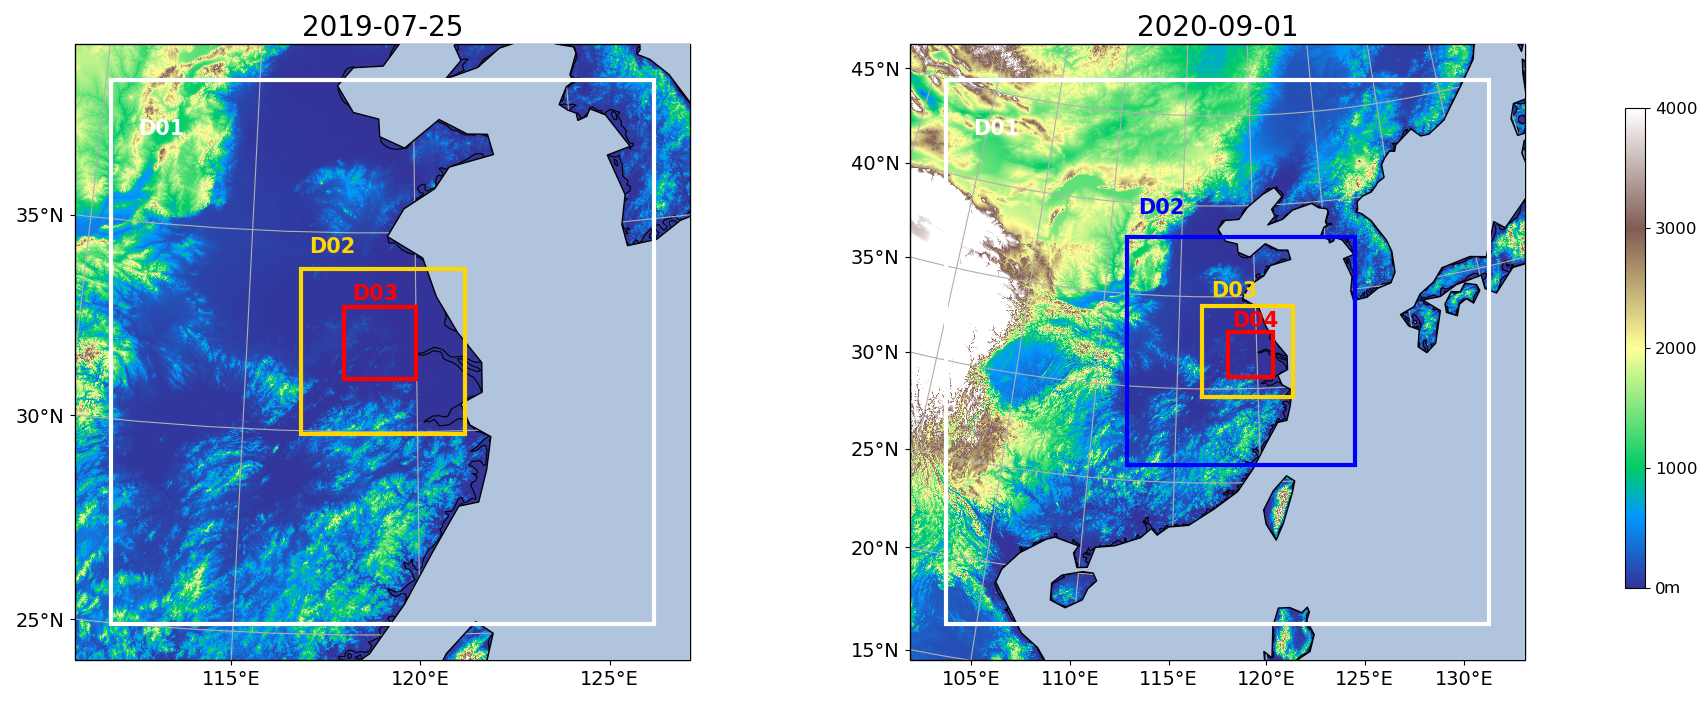
\includegraphics[width=0.9\textwidth]{./figures/domains_china.png}
\caption{2019年和2020年个例的WRF-Chem模拟区域和地形高度(m)图。
2019年个例的水平网格分辨率为15 km(D01)、3 km(D02)和 0.6 km(D03)。
对于2020年个例,分别为27 km(D01)、9 km(D02)、3 km(D03)和 1 km(D04)。\\
Figure \ref{fig:domains_china}. Domain and terrain height (m) of the WRF-Chem simulations for the 2019 and 2020 cases. The horizontal grid resolution of
domains for the 2019 case is 15 km (D01), 3 km (D02) and 0.6 km (D03). For the 2020 case, it is 27 km (D01), 9 km (D02), 3 km (D03),
and 1 km (D04).}
\label{fig:domains_china}
\end{figure}

\subsection{闪电氮氧化物的产率}

图\ref{fig:china_flash_scd}a--d将对流层NO$_2$斜柱浓度($S_{\ch{NO2}}$)的分布与观测的闪电分布进行了比较。
尽管由于探测器饱和和光晕效应,闪电最活跃像素上的$S_{\ch{NO2}}$无效,但对流附近或出流区仍有有效数据。
在2019年的个例中,闪电发生在TROPOMI过境前不到30分钟,
但2020年的个例中既有新生也有老化的LNO$_2$(图\ref{fig:china_flash_scd}d)。

具体而言,对流旺盛处(f$_r$ $\geq$ 0.7)的$S_{\ch{NO2}}$小于其他区域,
这与之前针对具有高闪电密度的大规模对流系统研究结果相反\citep{Beirle.2009},
导致这一差距的因素有四点:云顶高度、闪电次数、闪电发生时间和背景NO$_2$浓度。
由于TROPOMI只能探测到处于云层上方的LNO$_2$,因此当f$_r$ $\sim$ 1时,
闪电次数不足或对流较弱都可能导致对流旺盛区的$S_{\ch{NO2}}$更小。
即如果f$_r$<1,破碎或稀薄云层下方的部分污染NO$_2$会被TROPOMI探测到。
WRF-Chem的先验$S_{\ch{NO2}}$敏感性试验可以清楚地解释这种现象:
具有低f$_r$和高$S_{\ch{NO2}}$的像素源自于背景 NO$_2$ 污染(图\ref{fig:s5p_apriori_scd} a,e),
但与没有LNO$_2$贡献的低$S_{\ch{NO2}}$相比,对流层上层LNO$_2$增加的$S_{\ch{NO2}}$仍然可见(图\ref{fig:s5p_apriori_scd}b--d,f--h)。


在\ref{sec:us}节和\ref{sec:china}节中,我们利用对流旺盛时的卫星观测来估算 LNO$_x$产率。
然而由于 TROPOMI 的像素饱和和对流区域的有限覆盖(图\ref{fig:china_flash_scd}c),
该方法难以用于范围小发展强的对流(如2019年的个例)。
因此我们尝试不对云量加以限制,将该方法应用于消散期的对流(2020年个例,图\ref{fig:china_flash_scd}d)。
如图 \ref{fig:china_vcd_lnox}b--c 所示,闪电与TROPOMI的过境时间差大于 30 分钟但小于 3 小时。
由于 NO$_2$ 的寿命在对流附近为 $\sim$ 3(2--12)小时 \citep{Nault.2016},
2020年个例的TROPOMI观测数据仍可以用于估算LNO$_x$。
平均 LNO$_x$产率(mol/flash)的定义如下:
\begin{equation} \label{eq:lnox}
PE_{LNO_x} = \sum_{p} V_i A_i / \sum_{N} F_j e^{-(t_0 - t_j) / \tau}
\end{equation}
其中 $p$ 代表受 LNO$_x$ 影响的像素,
$V_i$(mol/m$^2$)是像素 $i$ 上LNO$_x$ 垂直柱浓度($V_{\ch{LNO_x}}$ = $S_{\ch{NO2}}$ / $AMF_{\ch{LNO_x}}$),
面积称为 A$_i$ (m$^2$),
$N$ 是 对 $V_{\ch{LNO_x}}$ 做出贡献的闪电总数,
指数部分考虑了每个闪电(F$_j$)排放的NO$_x$ 的寿命。
具体而言AMF$_{\ch{LNO_x}}$源于式(\ref{eq:AMF_LNO2}),
t$_0$是TROPOMI的过境时间,
t$_j$是闪电的发生时间,
$\tau$为近对流的NO$_x$寿命(3 小时)。


\begin{figure}[H]
    \centering
    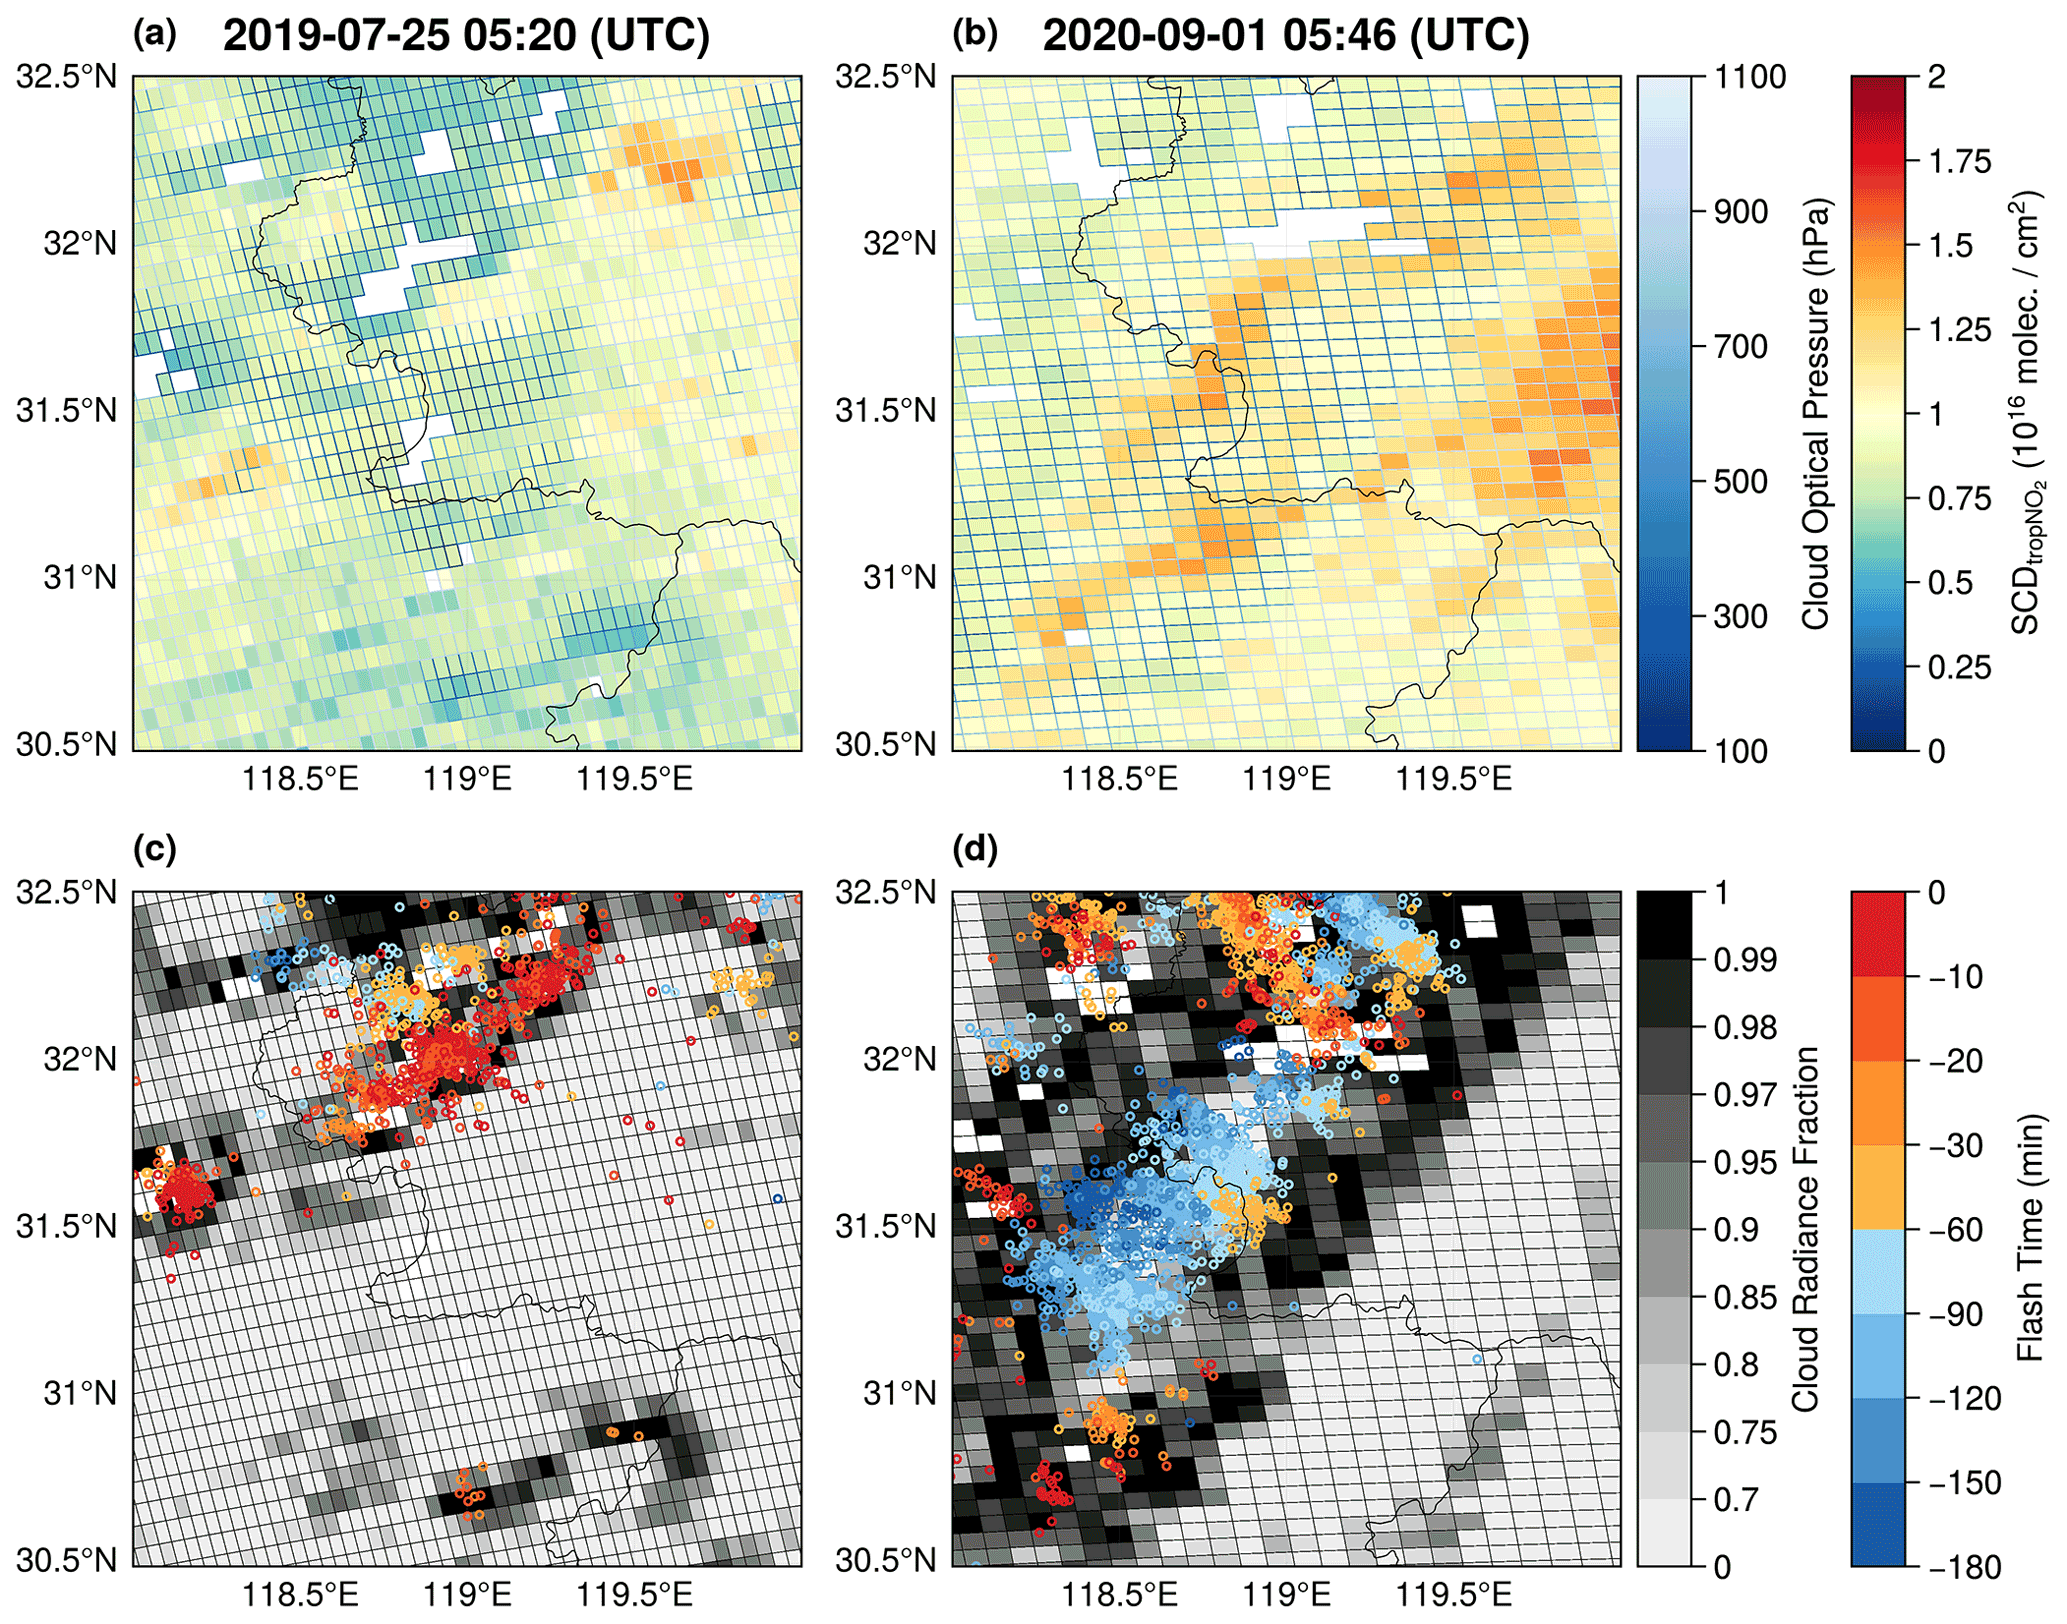
\includegraphics[width=0.8\textwidth]{./figures/china_flash_scd.png}
    \caption{
    2019 年 7 月 25 日(左)和 2020 年 9 月 7 日(右)的个例。
    (a,b)对流层 NO$_2$ 斜柱浓度($S_{\ch{NO2}}$,填充色)和云压(线条颜色)。
    白色网格代表缺失的 TROPOMI 数据,黑色实线为江苏省;
    (c,d)NO$_2$ 窗区中的云辐射分数和闪电。闪电的颜色取决于相对于TROPOMI过境的发生时间。\\
    Figure \ref{fig:china_flash_scd}. Events on 25 July 2019 (left) and 07 September 2020 (right).
    (a, b) The tropospheric NO$_2$ slant column density ($S_{\ch{NO2}}$, filled color) and cloud optical pressure (line color).
    These white grid cells stand for missing TROPOMI data.
    The solid black border is Jiangsu province.
    (c, d) The cloud radiance fraction in the NO$_2$ window and flashes whose color depends on the occurring time relative to the TROPOMI overpass time.
    }
    \label{fig:china_flash_scd}
\end{figure}


\begin{sidewaysfigure}[!htbp]
    \centering
    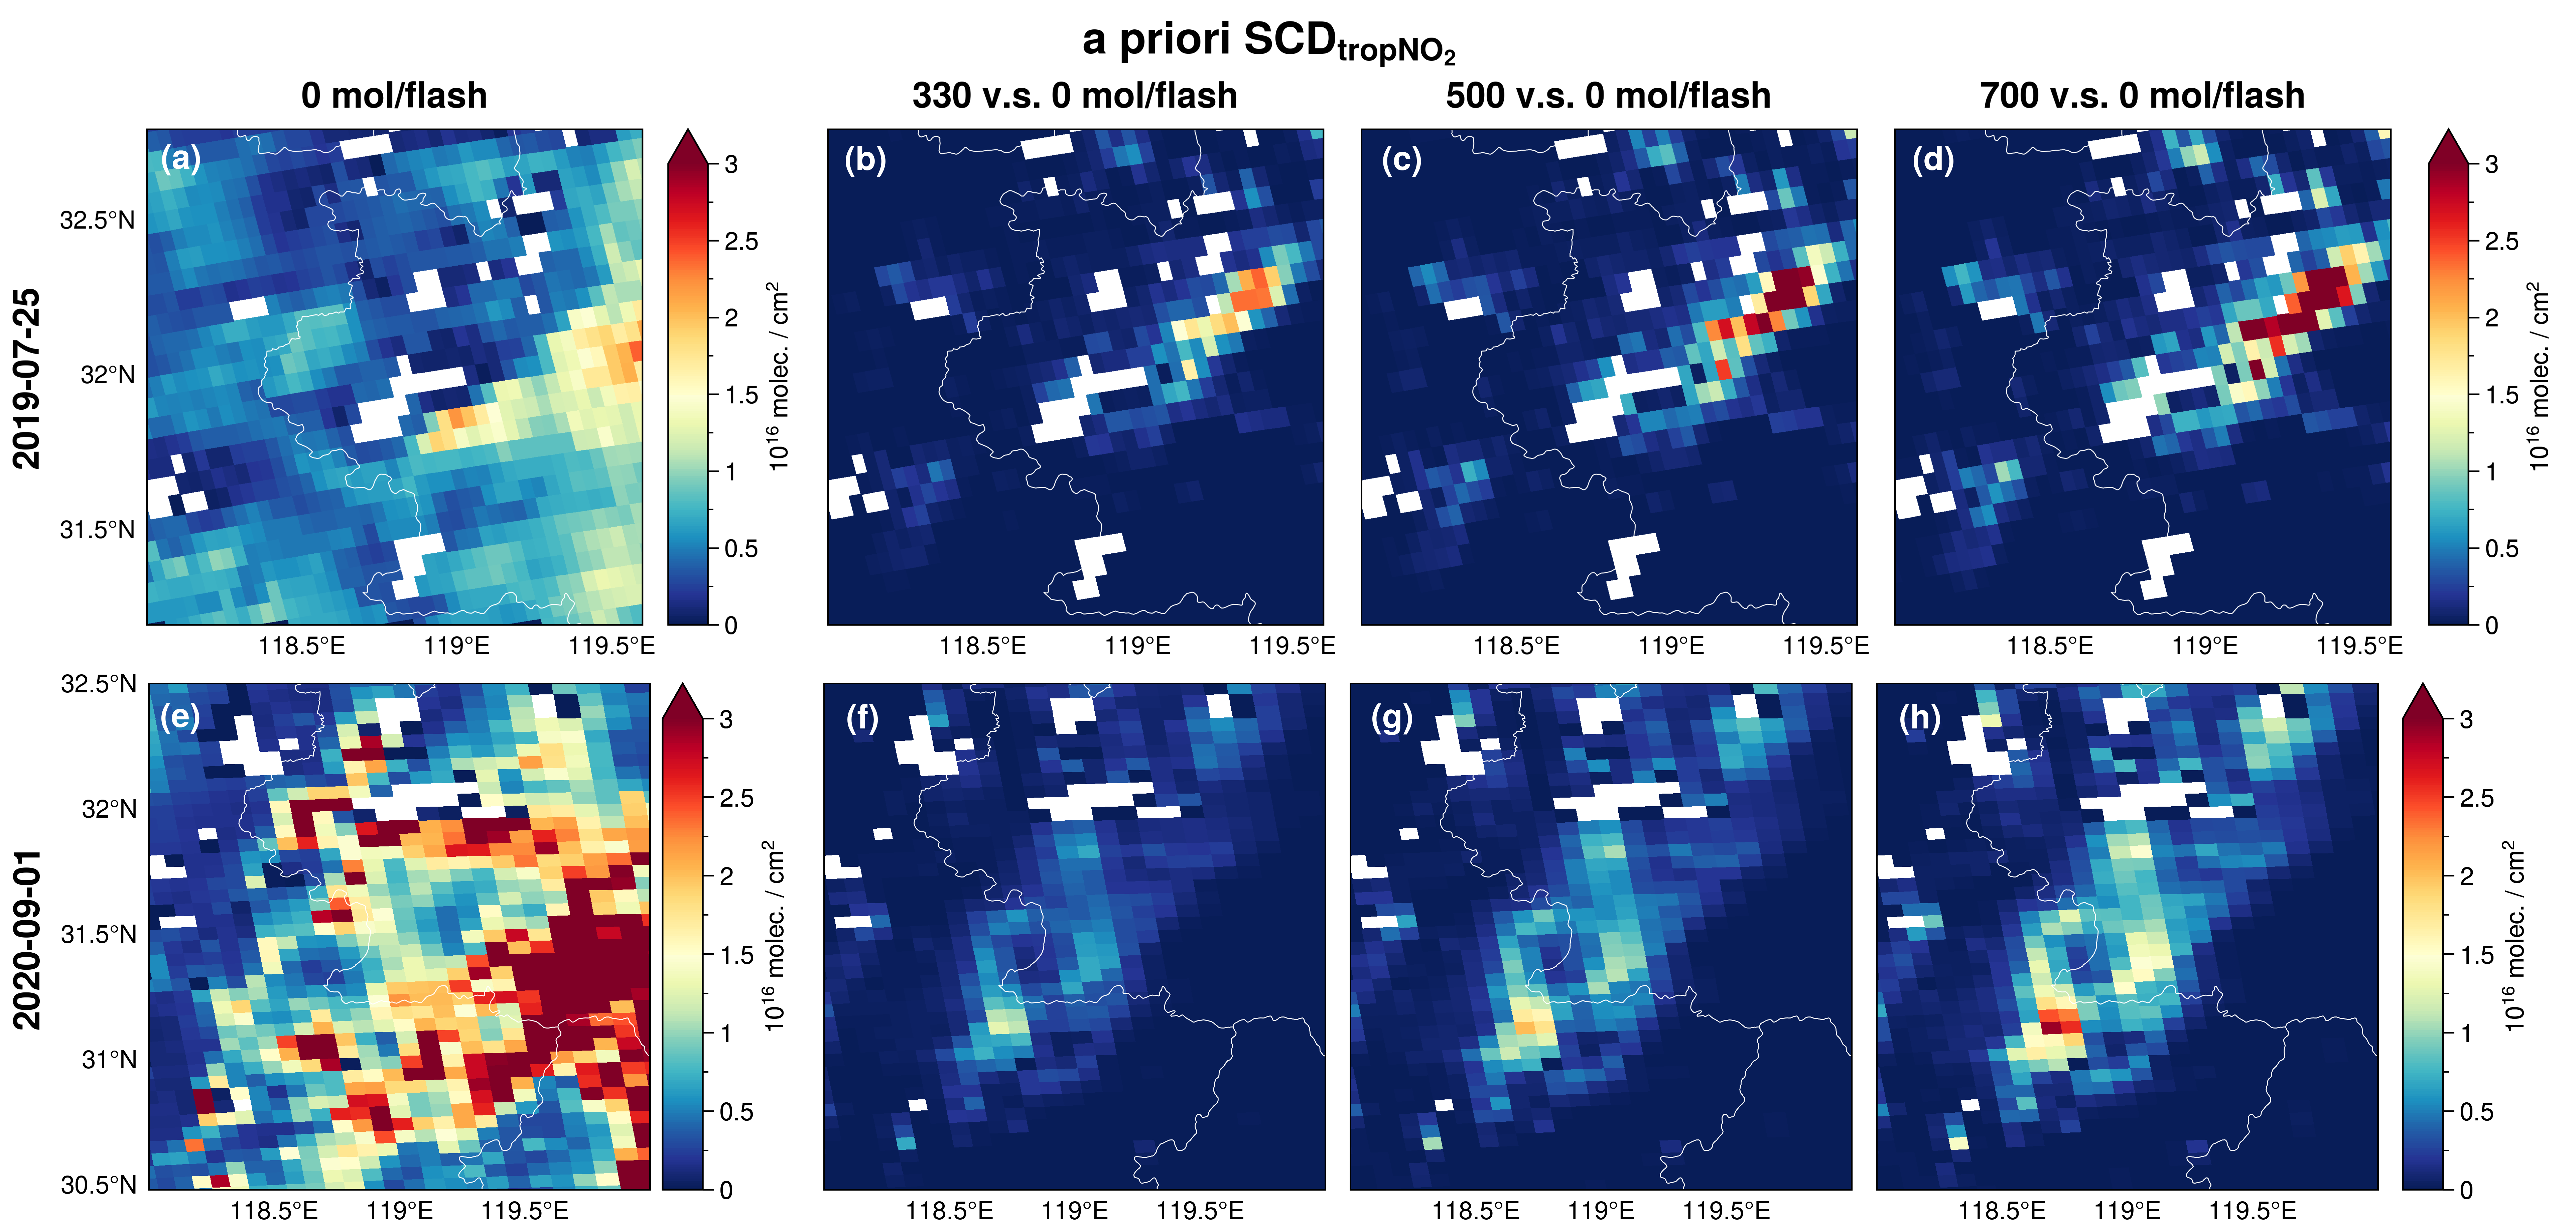
\includegraphics[width=0.85\columnwidth]{./figures/s5p_apriori_scd.png}
    \caption{使用不同闪电NO排放条件下WRF-Chem的NO$_2$结果,重新计算得到的对流层NO$_2$斜柱浓度($S_{\ch{NO2}}$)。
    (a,e)0 mol每闪电;(b,f)330 mol每闪电;(c,g)500 mol每闪电;(d,h)700 mol每闪电。\\
    Figure \ref{fig:s5p_apriori_scd}. The tropospheric NO$_2$ slant column density ($S_{\ch{NO2}}$) recalculated using the WRF-Chem results with different lightning NO settings: (a, e) 0 mol/flash, (b, f) 330 mol/flash, (c, g) 500 mol/flash and (d, h) 700 mol/flash.
    }
    \label{fig:s5p_apriori_scd}
\end{sidewaysfigure}
\FloatBarrier

由于消散的对流在旺盛期间已产生了足够多的闪电,并且对流处对流层上层的风从西北偏西吹向东南偏东(图\ref{fig:china_vcd_lnox}a),
$V_{\ch{LNO_x}}$的范围仍然可以清楚地识别(图\ref{fig:china_vcd_lnox} 中的虚线矩形),且有一条$V_{\ch{LNO_x}}$低值带将南北对流分开。
经过仔细选择,计算得到的LNO$_x$产率为60 mol NO$_x$每闪电。
虽然有些与 $V_{\ch{LNO_x}}$ 相关的闪电在选择的区域之外,
它对LNO$_x$产率的影响仅 $\sim$ 2 mol,在下节的不确定性评估范围内。


\begin{figure}[H]
    \centering
    
\includegraphics[width=\textwidth]{./figures/china_vcd_lnox.png}
    \caption{
    背景为LNO$_x$垂直柱浓度($V_{\ch{LNO_x}}$)的分布。
     白色矩形是为手动选择用于 LNO$_x$产率估算的区域。
     (a)中叠加的箭头是 WRF-Chem 模拟的 500 hPa 水平风;
     (b)和(c)中的点是闪电,其颜色取决于相对于 TROPOMI 过境的发生时间。\\
    Figure \ref{fig:china_vcd_lnox}. The background is the distribution of LNO$_x$ vertical column densities ($V_{\ch{LNO_x}}$).
    The white rectangles are manually selected regions for the LNO$_x$ production efficiency estimation.
    The overlayed wind arrows in (a) are the 500 hPa horizontal wind simulated by WRF-Chem.
    The dots in (b) and (c) are the flashes whose color depends on the occurring time relative to the TROPOMI overpass time.
    }
    \label{fig:china_vcd_lnox}
\end{figure}


\subsection{估算的影响因素及不确定性分析} \label{sec:uncertainty_china}

根据 \citet{Allen.2019} 和 \citet{Zhang.2020b},LNO$_x$ 的不确定性由 LNO$_x$ 寿命、闪电探测效率、
NO/NO$_2$ 比例、LNO 廓线和其他来源决定(表\ref{table:uncertainty_china})。
我们将NO$_2$的寿命替换为2 和6 h,得到的不确定性为27\%,而将IC与CG的比值改为2 :1 和 4:1,得到的不确定性也为27\%。
根据 \citet{Allen.2019} 我们将由模拟引起的 NO/NO$_2$ 比例的不确定性设置为 30\%。
此外我们利用330 和 700 mol NO每闪电的WRF-Chem敏感性试验结果,得到与LNO廓线有关的不确定性为 26\%。
此外,与平流层垂直柱浓度[$\pm$ 10$^{14}$ molec. cm$^2$, \citet{VanGeffen.2022}]相关的不确定性为 7\%。
而由其他可能误差源引起的不确定性难以量化,比如斜柱浓度中的系统误差、云压和由对流重新分布的 NO$_2$,
根据 \citet{Allen.2021a}我们设其为10\%。
假设误差之间没有相关性,总不确定性(56\%)即为所有单个不确定性平方和的平方根。
因此LNO$_x$产率为60 $\pm$ 33 mol NO$_x$每闪电,
该数值低于我们(90 $\pm$ 50 mol NO$_x$每闪电)以及\citet{Allen.2021a}(120 $\pm$ 65 mol NO$_x$每闪电)在美国大陆的研究结果,
因此在未来的研究中还需对中国地区进行范围更广的探讨,从而估算区域性的LNO$_x$产率。


\begin{table}[H]
\footnotesize
\centering
\caption{LNO$_{\ch{x}}$产率估算的不确定性\\
Table \ref{table:uncertainty_china}. Uncertainties for the estimation of LNO$_\textrm{x}$ production efficiency.}
\begin{tabularx}{.8\textwidth}{c X}
\hline
来源 & \makecell[cc]{不确定性 (\%)} \\
\hline
LNO$_x$ 寿命                & \makecell[cc]{27\%} \\
闪电探测效率                  & \makecell[cc]{27\%} \\
NO/NO$_2$ 比例               & \makecell[cc]{30\%} \\
LNO 廓线                     & \makecell[cc]{26\%} \\
平流层垂直柱浓度                & \makecell[cc]{7\%} \\
其他                          & \makecell[cc]{10\%} \\
\hline
净不确定性                             & \makecell[cc]{56\%} \\
\hline
\end{tabularx}
\label{table:uncertainty_china}
\end{table}


\section{本章小结}

本章建立了基于卫星遥感NO$_2$柱浓度定量分析不同污染背景下LNO$_2$的
计算方法,得到了不同污染程度地区的LNO$_x$产率,并与其他NO$_x$排放源进行了对比。主要结论如下:

\begin{enumerate}[label=(\arabic*), labelindent=\parindent, leftmargin=0pt, widest=0, itemindent=*, topsep=0pt, partopsep=0pt, parsep=0pt]

\item 针对清洁地区(北极)的深对流,我们利用极轨卫星在北极地区连续过境的特性,
开发了TROPOMI LNO$_2$柱浓度高值区的自主识别系统,提出了通过相邻过境数据来定量计算 LNO$_2$ 寿命和产率的方法。

\item 2019至2021年6--8月的分析结果表明,北极地区对流附近的LNO$_2$寿命为3 h,
与污染地区的LNO$_2$寿命相似,例如美国地区的3 h \citep{Nault.2017}。
北极陆地地区的LNO$_2$ 产率 [2.0(1.3--3.1)mol每闪击] 与美国的结果(1.6 $\pm$ 0.1 mol每闪击)也相近\citep{Lapierre.2020}。
此外北极海洋性闪电产生的 NO$_2$是陆地性闪电的6倍,
因此当闪电在北极海洋和陆地上增加相同数量时,海洋性闪电将产生更多的 LNO$_2$。
基于得到的LNO$_2$产率,我们进一步得出北极地区夏季(6--8 月)LNO$_x$ 的平均排放量为219吨氮,
约等于该地区人为 NO$_x$ 排放量的 5\%。

\item 针对污染地区的深对流,我们利用WRF-Chem的高分辨率模拟结果,
定义了LNO$_2$和LNO$_x$的大气质量因子(AMF),
从而得到包含了云下LNO$_2$和LNO$_x$的柱浓度。
% 我们利用云辐射分数、地基探测的闪电阈值、模拟的闪电数$\geq$1000 和云上LNO$_2$占比$\geq$50\%来确保WRF-Chem 成功模拟出对流并且LNO$_2$能够被OMI检测。
由于新定义的AMF考虑了对流层的背景污染,因此该方法同时适用于清洁和污染区域。

\item 2014年5--8月的分析结果表明,美国大陆夏季的 LNO$_2$ 和 LNO$_x$平均产率为
32 $\pm$ 15 mol NO$_2$每闪电、90 $\pm$ 50 mol NO$_x$每闪电、6 $\pm$ 3 mol NO$_2$每闪击,以及17 $\pm$ 10 mol NO$_x$每闪击。
由于现阶段其他地区(如中国和印度)NO$_2$ 污染比美国大陆严重,因此LNO$_x$的估算有必要详细考虑NO$_2$背景污染。
此外区域和全球模式还需开发更为完善的闪电参数化,进而提高局地和全球范围内LNO$_x$排放估算的准确性。

\item 2019年和2020年中国东南部的两个对流个例分析表明,TROPOMI 的像素饱和效应导致无法获得旺盛对流处的LNO$_x$,
因此我们提出计算消散阶段的LNO$_x$,并得到中国东南部的LNO$_x$产率为 60 $\pm$ 33 mol NO$_x$每闪电。
未来的研究可同时利用旺盛和消散对流期间 OMI或TROPOMI 的有效数据,从而量化和改进 LNO$_x$ 的产量估计。

\end{enumerate}
